%%!TEX encoding = UTF-8 Unicode

% Several lines in file have comments suggesting common packages for the
% typical thesis in informatics or electronics developed at UA
% uncomment/comment the lines as required for your work
% Before each optional line you will have a small comment

% According to UA rules, font size should range from 10 to 12pt.
\documentclass[11pt,a4paper,openright,twoside,onecolumn]{memoir}

\listfiles
\fixpdflayout

\usepackage[utf8]{inputenc}

% Select Computer Modern Typewritter (For bold ttfamily in listings)
\usepackage{lmodern}
% OR... Bera Mono
%\usepackage[scaled]{beramono} % TTT Font
%\usepackage{anyfontsize} % As the name says...

\usepackage[T1]{fontenc}

% Enable for for Overleaf support
\usepackage{ifthen}
\def\useoverleaf{1}  % change to non-zero (for instance, 1) to enable it

\makeatletter
\newcommand{\makecoverfile}[0]{%
  \immediate\write18{latexmk -pdf cover.tex}%
}
\makeatother

% For PDF merging
\usepackage{pdfpages}

% Set DPI to 300
\pdfpxdimen=\dimexpr 1in/300\relax

% Allow the use of a larger number of packages
\usepackage{morewrites} 

% For English and Portuguese languages
% Portuguese will be the default.
% Uncomment \setlanguage below to change it
\usepackage[english,portuguese]{babel}

% Uncomment to use a custom date format
%\usepackage{datetime}
%\newdateformat{thesisdate}{\monthname[\THEMONTH] \THEYEAR} % Month Year

% Make pdf look better
\usepackage{microtype} 

% Uncomment to enable floats on facing pages
%\usepackage{dpfloat}

% Side by side figures
% Eg. Fig 1a, Fig 1b
\usepackage[hang,small,bf]{caption}
%\let\tion\undefined
%\let\subfloat\undefined
\usepackage{subcaption}

%\RequirePackage{textcase}

% Dropped Caps
%\usepackage{lettrine}

% Configure Hyperlink color
% As a matter or style, you may use this to enable/disable color boxes on links
%\usepackage[breaklinks=true,colorlinks=false,linkcolor=blue]{hyperref}
% Or use the default values provided by the hyperref package
\usepackage{hyperref}

% Redefine section names according to your preference
%\def\sectionautorefname{Section}
%\def\chapterautorefname{Chapter}
%\def\figureautorefname{Figure}
%\def\listingautorefname{Listing}
%\def\tableautorefname{Table}

% Redefine code boxes
\ifthenelse{\equal{\useoverleaf}{0}}
{\usepackage[outputdir=build]{minted}}
{\usepackage{minted}}%

\addto\captionsportuguese{%
  \renewcommand\listingscaption{Código}
}
\fvset{fontsize=\footnotesize} % Make Code blocks smaller than text
\usepackage{csquotes}

% Add support for PDF Comments
\usepackage{comment}
\ifthenelse{\equal{\useoverleaf}{0}}
{\usepackage{pdfcomment}}{}
\usepackage{bookmark} % New Bookmarks

% For Multiple columns in Glossary
\usepackage{multicol}

% Add support for Math symbols
\usepackage{amsmath}
\usepackage{amssymb}

% Add support for graphics
\usepackage{graphicx}

% Add support for Colors
\usepackage{xcolor}

% Add support for the Euro symbol
\usepackage{eurosym}

% Add support for missingfigure and todo
\usepackage{todonotes}

% Setup bibliography with Biber using IEEE style for proper UTF-8 support
\usepackage[backend=biber, style=ieee, sorting=none, natbib=true, mincitenames=1, maxcitenames=2]{biblatex}
\bibliography{bib/references.bib, bib/rfc.bib}

% Use acronyms
\usepackage[printonlyused]{acronym} % For acronyms

% Indenting the first paragraph after section start
\usepackage{indentfirst}

% For fixing listoflistings with memoir
\usepackage{xparse}

% Uncomment the next lines to enable chart support through pgf and tikz
% This may require you to install further packages in your Tex system
%\usepackage[version=0.96]{pgf}
%\usepackage{tikz}

% UML support
%\usepackage{pgf-umlsd}

% Trees, Arrows, Mindmaps and other popular objects
%\usetikzlibrary{arrows,shadows,trees,shapes,decorations,automata,backgrounds,petri,mindmap} % for pgf-umlsd

% Package to master SI units
\usepackage[detect-weight=true, binary-units=true]{siunitx}
% For Electric Circuits
%\sisetup{load-configurations = binary}

% Set Voltage direction accordingly
% Option : oldvoltagedirection,nooldvoltagedirection,RPvoltages,EFvoltages
% More information at: https://mirrors.ibiblio.org/CTAN/graphics/pgf/contrib/circuitikz/doc/circuitikzmanual.pdf
% By default this template is using the Old Voltage Direction
%\usepackage[oldvoltagedirection,american,cuteinductors,smartlabels]{circuitikz}
%\usetikzlibrary{calc}
%\ctikzset{bipoles/thickness=1}
%\ctikzset{bipoles/length=0.8cm}
%\ctikzset{bipoles/diode/height=.375}
%\ctikzset{bipoles/diode/width=.3}
%\ctikzset{tripoles/thyristor/height=.8}
%\ctikzset{tripoles/thyristor/width=1}
%\ctikzset{bipoles/vsourceam/height/.initial=.7}
%\ctikzset{bipoles/vsourceam/width/.initial=.7}
%\tikzstyle{every node}=[font=\small]
%\tikzstyle{every path}=[line width=0.8pt,line cap=round,line join=round]

% For inline TT text (e.g. code snippets)
\usepackage{verbatim}

% Frames around figures and allow force placement
\usepackage{float}

% Configure Float style
%\floatstyle{boxed}
%\restylefloat{table}
%\restylefloat{figure}
%\restylefloat{lstlisting}

% For test purposes you may use the lipsum package to create dummy text
\usepackage{lipsum} % REMOVE

%Keep floats inside section!
\usepackage[section]{placeins}
\let \oldsubsubsection \subsubsection
\renewcommand{\subsubsection}[2][]{
  \FloatBarrier
  \oldsubsubsection#1{#2}
}
\let \oldsubsection \subsection
\renewcommand{\subsection}[2][]{
  \FloatBarrier
  \oldsubsection#1{#2}
}
\let \oldsection \section
\renewcommand{\section}[2][]{
  \FloatBarrier
  \oldsection#1{#2}
}
\let \oldchapter \chapter
\renewcommand{\chapter}[2][]{
  \FloatBarrier
  \oldchapter#1{#2}
}



% Use the built-in division styling
\headstyles{memman}

% Include subsections in the TOC
\settocdepth{subsection}

% Numbering down to subsections as well
\setsecnumdepth{subsection}

% extra index for first lines
\makeindex[lines]

% Margins for University of Aveiro Thesis
\setlrmarginsandblock{3cm}{2.5cm}{*}
\setulmarginsandblock{3cm}{3cm}{*}
\checkandfixthelayout

% Or select your custom spacing to make any ajustment
%\addtolength{\parskip}{0.5\baselineskip}
\linespread{1.5}

\newcommand\mainmatterWithoutReset
{\edef\temppagenumber{\arabic{page}}%
  \mainmatter
  \setcounter{page}{\temppagenumber}%
}


%%%%%%%%%%%%%%%%%%%%%%%%%%%%%%%%%%%%%%%%%%%%%%%%%%
% Document begins here
%%%%%%%%%%%%%%%%%%%%%%%%%%%%%%%%%%%%%%%%%%%%%%%%%%

\begin{document}
\ifthenelse{\equal{\useoverleaf}{0}}{}{\makecoverfile{}}%
\includepdf[pages=-]{cover.pdf}

% Uncomment to enable English
\selectlanguage{english}


% Front matter

%Custom Chapter style named `thesis`
\makechapterstyle{thesis}{% Based on ell
  \chapterstyle{default}
  \renewcommand*{\chapnumfont}{\normalfont\sffamily}
  \renewcommand*{\chaptitlefont}{\normalfont\Huge\sffamily}
  \settowidth{\chapindent}{\chapnumfont 111}
  \renewcommand*{\chapterheadstart}{\begingroup
    \vspace*{\beforechapskip}%
    \begin{adjustwidth}{}{-\chapindent}%
    \hrulefill
    \smash{\rule{0.4pt}{15mm}}
    \end{adjustwidth}\endgroup}
  \renewcommand*{\printchaptername}{}
  \renewcommand*{\chapternamenum}{}
  \renewcommand*{\printchapternum}{%
    \begin{adjustwidth}{}{-\chapindent}
    \hfill
    \raisebox{10mm}[0pt][0pt]{\fontsize{30}{25}\selectfont\chapnumfont \thechapter}%
                              \hspace*{1em}
    \end{adjustwidth}\vspace*{-3.0\onelineskip}}
  \renewcommand*{\printchaptertitle}[1]{%
    \vskip\onelineskip
    \raggedleft {\chaptitlefont ##1}\par\nobreak\vskip 4\onelineskip}}


% Select chapter style from existing or select custom
%\chapterstyle{thesis} % Others: dowding, demo2, dash, chappell, brotherton, bianchi, ger, madsen, tatcher, veelo,indexes)
% thesis can also be used as defined previously
% Check the memoir documentation for the available themes
% Default is veelo
\chapterstyle{veelo}
\makeoddfoot{plain}{}{\thepage}{} % Added by André Zúquete to fix a page numbering issue on the veelo chapter style


% If you feel adventurous you can also define all aspects of your theme
% Use either this input or the chapterstyle before
% % Rules
\newcommand{\thinRule}{\rule{\textwidth}{0.25pt}}

% Customize heading appearances
% Define styles
\newcommand{\partSize}{\Huge}
\newcommand{\partStyle}{\lsstyle\scshape}
\newcommand{\chapterSize}{\Huge}
\newcommand{\chapterStyle}{\lsstyle\scshape}
\newcommand{\chapterAfter}{}
\newcommand{\sectionSize}{\Large}
\newcommand{\sectionStyle}{\scshape\MakeTextLowercase}
\newcommand{\subsectionSize}{\large}
\newcommand{\subsectionStyle}{\scshape\MakeTextLowercase}
\newcommand{\subsubsectionSize}{\large}
\newcommand{\subsubsectionStyle}{\scshape\MakeTextLowercase}
\newlength{\partNumSizePt}
\setlength{\partNumSizePt}{60pt}
\newlength{\chapterNumSizePt}
\setlength{\chapterNumSizePt}{60pt}
\newcommand{\partNumSize}{%
  \fontsize{\partNumSizePt}{1.2\partNumSizePt}\selectfont%
}
\newcommand{\partNumStyle}{\partChapterNumColor}
\newcommand{\chapterNumSize}{%
  \fontsize{\chapterNumSizePt}{1.2\chapterNumSizePt}\selectfont%
}
\newcommand{\chapterNumStyle}{\partChapterNumColor}

% Customize parts
\renewcommand{\partnamefont}{\partSize\partStyle}
\renewcommand{\partnumfont}{\partNumSize\partNumStyle}
\renewcommand{\printpartname}{}
\renewcommand{\printparttitle}[1]{%
  \normalfont\normalcolor\partnamefont #1
}

% Customize chapters
\makeatletter
\setlength{\beforechapskip}{30pt}
\renewcommand*{\chapterheadstart}{\vspace*{\beforechapskip}}
\setlength{\afterchapskip}{3ex}
\setlength{\midchapskip}{3ex}
\renewcommand*{\chapnamefont}{%
  \Large\flushright\chapterStyle\partChapterNumColor%
}
\renewcommand*{\chapnumfont}{\chapterNumSize\chapterNumStyle}
\renewcommand*{\chaptitlefont}{%
  \normalfont\flushleft\normalcolor\chapterSize\chapterStyle%
}
\renewcommand*{\printchaptername}{%
  \chapnamefont\MakeTextLowercase{\@chapapp}%
}
\renewcommand*{\chapternamenum}{\quad}
\renewcommand*{\printchapternum}{%
%  \chapnumfont\textls[-75]{\classicstylenums{\thechapter}}%
 \chapnumfont\textls[-75]{\thechapter}%

}
\renewcommand*{\printchaptertitle}[1]{%
  \chaptitlefont #1
  \chapterAfter
}
\makeatother
% Customize sections and subsections
\setsecnumformat{\csname my#1\endcsname\quad}
\setsecheadstyle{\sectionSize\sectionStyle}
\newcommand{\mysection}{{\thesection}}
\setlength{\beforesecskip}{3em}


\setsubsecheadstyle{\subsectionSize\subsectionStyle}
\newcommand{\mysubsection}{{\normalfont\subsectionSize\thesubsection}}
\setlength{\beforesubsecskip}{3em}

\setsubsubsecheadstyle{\subsubsectionSize\subsubsectionStyle}
\newcommand{\mysubsubsection}{{\normalfont\subsubsectionSize\thesubsubsection}}
\setlength{\beforesubsubsecskip}{2em}

% Customize "Table of ..." appearance
% Customize headings
\newcommand{\renewPrintXTitle}[1]{%
  \renewcommand{#1}[1]{%
    \printchaptertitle{##1}%
  }%
}
\renewPrintXTitle{\printtoctitle}
\renewPrintXTitle{\printlottitle}
\renewPrintXTitle{\printloftitle}

% Customize ToC headings
\renewcommand{\cftpartfont}{\partChapterNumColor\partStyle}
\renewcommand{\cftchapterfont}{\chapterStyle}
\renewcommand{\cftsectionfont}{}
\renewcommand{\cftsubsectionfont}{}
\renewcommand{\cftfigurefont}{}
\renewcommand{\cfttablefont}{}
\newcommand{\cftlstlistingfont}{}

% Increase number width
\newlength{\cftNumWidthIncrease}
\setlength{\cftNumWidthIncrease}{0.25em}
\addtolength{\cftpartnumwidth}{\cftNumWidthIncrease}
\addtolength{\cftchapternumwidth}{\cftNumWidthIncrease}
\addtolength{\cftsectionindent}{\cftNumWidthIncrease}
\addtolength{\cftsubsectionindent}{\cftNumWidthIncrease}
% No leader dots
%\renewcommand*{\cftpartdotsep}{\cftnodots}
%\renewcommand*{\cftchapterdotsep}{\cftnodots}
%\renewcommand*{\cftsectiondotsep}{\cftnodots}
%\renewcommand*{\cftsubsectiondotsep}{\cftnodots}
%\renewcommand*{\cftfiguredotsep}{\cftnodots}
%\renewcommand*{\cfttabledotsep}{\cftnodots}
%\newcommand*{\cftlstlistingdotsep}{\cftnodots}
% Set page numbers immediately after entry text
\newcommand{\tocEntryPageSep}{\hspace{1em}}
\renewcommand{\cftpartleader}{\cftdotfill{\cftdotsep}}
%\renewcommand{\cftpartafterpnum}{\cftparfillskip}
%\renewcommand{\cftchapterleader}{\tocEntryPageSep}
\renewcommand{\cftchapterleader}{\cftdotfill{\cftdotsep}}
%\renewcommand{\cftchapterafterpnum}{\cftparfillskip}
\renewcommand{\cftsectionleader}{\cftdotfill{\cftdotsep}}
%\renewcommand{\cftsectionafterpnum}{\cftparfillskip}
\renewcommand{\cftsubsectionleader}{\cftdotfill{\cftdotsep}}
%\renewcommand{\cftsubsectionafterpnum}{\cftparfillskip}
\renewcommand{\cftfigureleader}{\cftdotfill{\cftdotsep}}
%\renewcommand{\cftfigureafterpnum}{\cftparfillskip}
\renewcommand{\cfttableleader}{\cftdotfill{\cftdotsep}}
%\renewcommand{\cfttableafterpnum}{\cftparfillskip}
\newcommand{\cftlstlistingleader}{\cftdotfill{\cftdotsep}}
%\newcommand{\cftlstlistingafterpnum}{\cftparfillskip}
% Customize page numbers
\newcommand{\tocPageStyle}{\tocPageColor}
\renewcommand{\cftpartpagefont}{\tocPageStyle}
\renewcommand{\cftchapterpagefont}{\tocPageStyle}
\renewcommand{\cftsectionpagefont}{\tocPageStyle}
\renewcommand{\cftsubsectionpagefont}{\tocPageStyle}
\renewcommand{\cftfigurepagefont}{\tocPageStyle}
\renewcommand{\cfttablepagefont}{\tocPageStyle}
\newcommand{\cftlstlistingpagefont}{\tocPageStyle}

% Abstract
% Remove indents around abstract text
\setlength{\absleftindent}{0pt}
\setlength{\absrightindent}{0pt}
% Change font size to conform with the rest of the document text
\renewcommand{\abstracttextfont}{\normalsize}

% Customize headers and footers including page numbers
\newcommand{\hfTextSize}{\footnotesize}
\newcommand{\headTextStyle}{\lsstyle\scshape\MakeTextLowercase}
\nouppercaseheads
\makeevenhead{headings}%
             {\hfTextSize\thepage}%
             {}%
             {\hfTextSize\headTextStyle\leftmark}
\makeevenhead{plain}%
             {\hfTextSize\thepage}%
             {}%
             {\hfTextSize\headTextStyle\leftmark}
\makeoddhead{headings}%
            {\hfTextSize\headTextStyle\rightmark}%
            {}%
            {\hfTextSize\thepage}
\makeoddhead{plain}%
            {\hfTextSize\headTextStyle\rightmark}%
            {}%
            {\hfTextSize\thepage}


% Customize captions
\newcommand{\captionSize}{\small}
\newcommand{\captionStyle}{\scshape}
\newcommand{\captionWidthRatio}{0.9}

\captionnamefont{\captionSize\captionStyle}
\captiontitlefont{\captionSize}
\captiondelim{ -- }
\captiontitlefinal{}
\changecaptionwidth
%\captionwidth{\captionWidthRatio\textwidth}

% Define colors
%\newcommand{\titleColor}{\color[rgb]{0.616, 0.0627, 0.176}}
\newcommand{\titleColor}{\color[rgb]{0,0,0}}

\newcommand{\partChapterNumColor}{\titleColor}
\newcommand{\dropCapColor}{\titleColor}
%\newcommand{\tocPageColor}{\color[rgb]{0.0980, 0.329, 0.651}}

\newcommand{\tocPageColor}{\color[rgb]{0, 0,0}}
\definecolor{shade0}{rgb}{1.0 , 1.0 , 1.0 }
\definecolor{shade1}{rgb}{0.9 , 0.9 , 0.9 }
\definecolor{shade2}{rgb}{0.8 , 0.8 , 0.8 }
\definecolor{shade3}{rgb}{0.65, 0.65, 0.65}
\definecolor{shade4}{rgb}{0.45, 0.45, 0.45}
\definecolor{shade5}{rgb}{0.0 , 0.0 , 0.0 }



%Exclude sub figures from List of Figures
%\captionsetup[subfloat]{list=no}

% Texts
\newenvironment{introduction}
{%
  \begin{minipage}{\textwidth}%
   \itshape%
}
{%
  \end{minipage}%
  \par\addvspace{2\baselineskip plus 0.2\baselineskip minus 0.2\baselineskip}%
}

% Select Page style
\pagestyle{plain}


\frontmatter

\tightlists
\midsloppy
\raggedbottom

\setcounter{tocdepth}{2} %subsections are added to the TOC
\setcounter{secnumdepth}{4} %subsubsections are numbered

% Initial document tables start here: TOC, LOF, LOT, Glossary
% Table of contents with slightly smaller font
\cleardoublepage
{\small\tableofcontents}

% List of figures with slightly smaller font
\cleardoublepage
{\small\listoffigures}

% List of tables with slightly smaller font
%\cleardoublepage
%{\small\listoftables}

% List of code snippets

% Fix for Listings with memoir

\RenewDocumentCommand \chapter { s O{#3} m }{%
  \FloatBarrier
  \IfValueTF{#1}  % if optional star is seen
    {\oldchapter*{#2}}
    {\oldchapter#1{#2}}
}

\renewcommand{\listingscaption}{Código}
\renewcommand{\listoflistingscaption}{Lista de Excertos de Código}
%\cleardoublepage
%{\small\listoflistings}
%\addcontentsline{toc}{chapter}{\listoflistingscaption}

% Reset Chapters
\renewcommand{\chapter}[2][]{
  \FloatBarrier
  \oldchapter#1{#2}
}

% Print Glossary
{\small\chapter{Glossary}

\footnotesize
\SingleSpacing

\begin{multicols}{2}
\begin{acronym}[AAAAAA]

	% \acro{psu}[PSU]{Power Supply Unit}
	% \acro{psa}[PSA]{Phase Shift Array}
	% \acro{rf}[RF]{Radio Frequency}
 %        \acro{pcb}[PCB]{Printed Circuit Board}
 %        \acro{pa}[PA]{Power Amplifier}
 %        \acro{iq}[IQ]{In-phase / Quadrature}
 %        \acro{i}[I]{In-phase}
 %        \acro{q}[Q]{Quadrature}
 %        \acro{lo}[LO]{Local Oscillator}
 %        \acro{smps}[SMPS]{Switch-Mode Power Supply}
 %        \acro{dc}[DC]{Direct Current}
 %        \acro{ac}[AC]{Alternating Current}
 %        \acro{pwm}[PWM]{Pulse Width Modulation}
 %        \acro{bb}[BB]{Base Band}
 %        \acro{psk}[PSK]{Phase-Shift Keying}
 %        \acro{qpsk}[QPSK]{Quadrature Phase-Shift Keying}
 %        \acro{vcps}[VCPS]{Voltage Controlled Phase Shifter}
 %        \acro{imn}[IMN]{Input Matching Network}
 %        \acro{omn}[OMN]{Output Matching Network}
 %        \acro{fr}[$f_{R}$]{Resonance Frequency}
 %        \acro{if}[IF]{Intermediate Frequency}
 %        \acro{mmic}[MMIC]{Monolithic Microwave Integrated Circuit}
 %        \acro{mimo}[MIMO]{Multi-Input Multi-Output}
 %        \acro{qam}[QAM]{Quadrature Amplitude Modulation}
 %        \acro{par}[PAR]{Phased Array Radar}
 %        \acro{dsp}[DSP]{Digital Signal Processing}
 %        \acro{dbf}[DBF]{Digital Beamforming}
 %        \acro{fpga}[FPGA]{Field-Programmable Gate Array}
 %        \acro{ieee}[IEEE]{Institute of Electrical and Electronics Engineers }
 %        \acro{hpbw}[HPBW]{Half-Power Beamwidth}
 %        \acro{af}[AF]{Array Factor}
 %        \acro{qsll}[QSLL]{Quantization of Sidelobe Levels}
 %        \acro{iot}[IoT]{Internet of Things}
 %        \acro{siso}[SISO]{Single Input Single Output}
 %        \acro{mmse}[MMSE]{Minimum Mean Square Error}
 %        \acro{zf}[ZF]{Zero Forcing}
 %        \acro{snr}[SNR]{Signal-to-Noise Ratio}
 %        \acro{sinr}[SINR]{Signal-to-Interference-plus-Noise Ratio}
 %        \acro{los}[LOS]{Line of Sight}
 %        \acro{sumimo}[SU-MIMO]{Single User-MIMO}
 %        \acro{mumimo}[MU-MIMO]{Multiple User-MIMO}
 %        \acro{mmimo}[Massive MIMO]{Massive MIMO}
 %        \acro{ap}[AP]{Acess Point}
 %        \acro{sic}[SIC]{Successive Interferenc Cancellation}
 %        \acro{pic}[PIC]{Parallel Interference Cancellation}
 %        \acro{mud}[MUD]{Multi-User Detection}
 %        \acro{vswr}[VSWR]{Voltage Standing Wave Ratio}
 %        \acro{il}[IL]{Insertion Loss}
 %        \acro{spi}[SPI]{Serial Peripheral Interface}
 %        \acro{wlan}[WLAN]{Wireless Local Area Network}
\acro{ac}[AC]{Alternating Current}
\acro{af}[AF]{Array Factor}
\acro{ap}[AP]{Acess Point}
\acro{bb}[BB]{Base Band}
\acro{dbf}[DBF]{Digital Beamforming}
\acro{dc}[DC]{Direct Current}
\acro{dsp}[DSP]{Digital Signal Processing}
\acro{fpga}[FPGA]{Field-Programmable Gate Array}
\acro{fr}[$f_{R}$]{Resonance Frequency}
\acro{hpbw}[HPBW]{Half-Power Beamwidth}
\acro{ieee}[IEEE]{Institute of Electrical and Electronics Engineers }
\acro{if}[IF]{Intermediate Frequency}
\acro{i}[I]{In-phase}
\acro{ic}[IC]{Integrated Circuit}
\acro{il}[IL]{Insertion Loss}
\acro{imn}[IMN]{Input Matching Network}
\acro{iot}[IoT]{Internet of Things}
\acro{iq}[IQ]{In-phase / Quadrature}
\acro{lo}[LO]{Local Oscillator}
\acro{los}[LOS]{Line of Sight}
\acro{mmic}[MMIC]{Monolithic Microwave Integrated Circuit}
\acro{mmimo}[Massive MIMO]{Massive MIMO}
\acro{mmse}[MMSE]{Minimum Mean Square Error}
\acro{mimo}[MIMO]{Multi-Input Multi-Output}
\acro{mud}[MUD]{Multi-User Detection}
\acro{mumimo}[MU-MIMO]{Multiple User-MIMO}
\acro{par}[PAR]{Phased Array Radar}
\acro{pa}[PA]{Power Amplifier}
\acro{pcb}[PCB]{Printed Circuit Board}
\acro{pic}[PIC]{Parallel Interference Cancellation}
\acro{psa}[PSA]{Phase Shift Array}
\acro{psk}[PSK]{Phase-Shift Keying}
\acro{psu}[PSU]{Power Supply Unit}
\acro{pwm}[PWM]{Pulse Width Modulation}
\acro{q}[Q]{Quadrature}
\acro{qam}[QAM]{Quadrature Amplitude Modulation}
\acro{qpsk}[QPSK]{Quadrature Phase-Shift Keying}
\acro{qsll}[QSLL]{Quantization of Sidelobe Levels}
\acro{rf}[RF]{Radio Frequency}
\acro{sic}[SIC]{Successive Interferenc Cancellation}
\acro{siso}[SISO]{Single Input Single Output}
\acro{sinr}[SINR]{Signal-to-Interference-plus-Noise Ratio}
\acro{snr}[SNR]{Signal-to-Noise Ratio}
\acro{smps}[SMPS]{Switch-Mode Power Supply}
\acro{spi}[SPI]{Serial Peripheral Interface}
\acro{sumimo}[SU-MIMO]{Single User-MIMO}
\acro{vcps}[VCPS]{Voltage Controlled Phase Shifter}
\acro{vswr}[VSWR]{Voltage Standing Wave Ratio}
\acro{wlan}[WLAN]{Wireless Local Area Network}
\acro{zf}[ZF]{Zero Forcing}
\acro{omn}[OMN]{Output Matching Network}
\end{acronym}
\end{multicols}

}

%%%%%%%%%%%%%%%%%%%%%%%%%%%%%%%%%%%%%%%%%%%%%%%%%%%%%%%
% Main document starts here
%%%%%%%%%%%%%%%%%%%%%%%%%%%%%%%%%%%%%%%%%%%%%%%%%%%%%%%

\mainmatter

% Line spacing: 1.5 pt 
\OnehalfSpacing

%%%%%%%%%%%%%%%%%%%%%%%%%%%%%%%%%%%%%%%%%%%%%%%%%%%%%%%
% Start of Thesis text 
%%%%%%%%%%%%%%%%%%%%%%%%%%%%%%%%%%%%%%%%%%%%%%%%%%%%%%%

% Uncomment to add further chapters
\chapter{Introduction}
\label{chapter:introduction}


\section{Introduction}
\label{section:ch1_introduction}
\par In wireless communications, the ability to transmit more information is a growing demand for almost all applications. Technologies from cellular and \ac{wlan} systems, to the more recent 5G technology, and \ac{mimo} systems greatly benefit from improvements to their throughput and bandwidth. There is also the inherent necessity of controlling the direction of the beam being radiated from the antenna for specific applications, as is the case that was discussed during this dissertation. This allows for systems that can focus their beam and power radiated on a specific target area, instead of spending power radiating energy over a large area like conventional antennas. Nowadays there is also a growing concern to optimize systems so that their power consumption is the lowest it can be.

\par The solution that was studied and implemented during the course of this project is the usage of a matrix of small radiating elements. This array has the combined radiating power of the total vector sum of all the smaller radiating elements. This means that in certain places the interaction of their electromagnetic fields will be constructive, whilst on others it will be destructive.

\par In order to control the places of interaction of these electromagnetic fields, it is mandatory to control the phase of each individual matrix element. As such a \ac{psa} is the most suitable solution. In these arrays, we have several small antennas that act as a single large one. Each of these small radiating elements has a phase shifter, mixer, amplifier and antenna, among other circuits. This allowed for an external controller to change the offsets of each radiating element in order to form a beam towards a specific orientation by adjusting the constructive and destructive interactions of the several elements in the array.

\par The scope of this Master's Dissertation was to create a prototype for one element that can then be replicated into several others with a degree of accuracy and certainty to create a \ac{psa}.


\section{Motivation}
\label{section:ch1_motivation}

\par This project idea was conceived, in scope and specifications, so that the knowledge acquired during the course of the degree could be applied in a more practical way, while at the same time developing an engineering prototype that could be used as a proof of concept for a configurable, open source, and highly versatile \ac{psa} system for the Instituto de Telecomunicações.

\par While Instituto de Telecomunicações already owns a system capable of beam-forming, its closed source nature makes it immutable in configuration and does not allow any flexibility with respect to the way it can be assembled and rearranged.

\par The various topics lectured with regard to \ac{pcb} design, power converters, mixers, \ac{rf} amplifiers, \ac{rf} components and antennas were applied and the opportunity allowed them to be applied in a more engineering-focused setting and thus expanded upon.


\section{Specifications}
\label{section:ch1_specifications}

\par The initial specifications given for a single module are considered, as previously mentioned in \ref{section:ch1_motivation}, for a Master's Dissertation and are as follows.

\begin{itemize} 
    \item Occupy the smallest amount of space possible, while guaranteeing an appropriate geometry for a side-by-side mounting style in an array configuration;
    \item Incorporate a \ac{rf} \ac{pa} with adequate characteristics, an antenna and study the possibility of adding an \ac{rf} isolator in between the \ac{pa} and the antenna;
    \item A voltage controlled phase-shifter, that will be used by a controller in order to insert an adjustable offset on the phase of the carrier wave, as to configure the direction of the main beam to be radiated from the array;
    \item To have and \ac{iq} modulator calibrated to operate at a given frequency range;
    \item Each module will have to be simple to implement, with easily repeatable so that different replicas of the modules behave similarly to one another.
\end{itemize}

\par Furthermore other characteristics of the project were set as requirements.

\begin{itemize}
    \item The output power of the antenna should be in the range of $[5, 10]\:\si{W}$;
    \item The operating frequency of the \ac{rf} signal must be in the range of $[2.4; 5] \:\si{GHz}$;
    \item The \ac{iq} signals can have a bandwidth of up to $20 \:\si{MHz}$;
    \item The power fed to each module must come from a $28 \:\si{V}$ power source;
    \item The signal controlling the phase-sifter is in the range $[0, 28] \:\si{V}$.
\end{itemize}

\chapter{Context}
\label{chapter:ch2_context}

\par This chapter focuses on providing the reader with a general overview of the state of the art of wireless communications technologies, that are often used in tandem with \acl{psa}. The aim is to give the reader a fundamental understanding of the design and operation of these technologies, as well as some of the challenges that they are currently faced with. Throughout this chapter, there is a focus of reviewing the use of some of the more prominent technologies and techniques, specifically within the context of \ac{mimo} systems that are used in wireless communications and their ability to provide the user with high-speed and low-latency communications. These are more common and, as such, are of ever increasing interest of the engineering and scientific community in the field of consumer oriented services and goods.

\section{Phase Shifting}
\label{section:ch2_phase_shifting}

\par One of the main components of a \ac{psa} is the phase shifter. The component is used, as the name very directly implies, to shift the phase of a signal. As in all \ac{rf} elements there is a set of characteristics that the ideal phase shifter must have, such as having a precise offset range, in degrees,  that fits the desired application and having a null insertion loss (IL), measured in dB.

\par These devices can be controlled in three different forms. These can be mechanical, analog, or digital.

\par For mechanical phase shifters, it is necessary to physically change the position of a knob or a keyed slot, similar to potentiometers. 

\par An analogue phase shifter requires an analog signal to adjust the amount of degrees desired for the phase shift on the \ac{rf} signal. This control signal is usually a certain voltage that needs to be applied.

\par For digital phase shifters, to control the amount of shift applied to the \ac{rf} signal a digital control signal is used.

\par The utilization of a phase shifter requires some thought when it comes to where it is supposed to be used, as \cite{Mitilineos2005AImplementation} explains. Utilizing a phase shifter in \ac{if} or in \ac{bb} requires the addition of frequency converters that will not only increase the cost and implementation difficulty, but will also cost the phase of the initial signal intended to be phase shifted. Then it is best if we can operate the phase shifter at the desired \ac{rf}.

\par Internally, a phase shifter may utilize a series of components such as resistors, inductors, capacitors \cite{Mitilineos2005AImplementation} in order to create all-pass filters that induce phase shifts to the signal.

\par These can be implemented using \ac{mmic} technology. This approach is better than older distributed network solutions, as it provides a way to reduce the size of the physical phase shifter while allowing good performance, as explained in \cite{Koh20070.13-mArrays}. Although fine adjustments are difficult, the number of inductors needed for chips capable of small adjusments increases. As such, the usage of passive lumped components can become an issue with higher insertion losses that require the amplifiers within to compensate. This necessary corrections make it such that the good linearity and low power consumption in these passive systems is lost.

\par The approach used to correct these issues is to use transistors instead for differential phases \cite{Koh20070.13-mArrays}, each bit controlling a certain differential phase of the digital phase shifter. This way the phase shifter can have a decent amount of gain and accuracy, as well as the capability of fine control.

\section{Quadrature Modulation}
\par With the advent of wireless and wired telecommunications, the desire for higher bitrates arose when it comes to information transmission. In order to send more than one data stream per connection, several forms of encoding information were developed.

\par The focus of the study done is on the transmitter's perspective, thus the emphasis on modulation techniques instead of demodulation.

\par The encoding mentioned above is modulation, as \cite{Ha2010TheorySystems} mentions. Therefore, by proper modulation techniques, the symbols can be transmitted via a carrier sinusoidal wave. This modulation can be achieved through the manipulation of amplitude, phase or frequency of a carrier or through a combination of these.

\par Modulation types can usually be divided into two main categories \cite{Ha2010TheorySystems}, as explained. These forms of \ac{iq} modulation can be binary types of modulation like PSK, DPSK, ASK, FSK, MSK and GMSK or otherwise be M-ary modulation such as MASK, MPSK, DMPSK, MQAM, DMQAM, CSK, MFSK, CPM and OFDM.

\par For basic quadrature modulation, we can imagine the following case as suggested by \cite{Hanzo2011QuadratureEdition}. If we consider two data signals \ac{i} and \ac{q} and the carrier for \ac{lo} and that we can change the carrier phase from $0^{\circ}$ to $180^{\circ}$ meaning a logical 0 and logical 1 as in Figure \ref{fig:ch2_secMod_fig1} (a) and (b). If the original data set to be encoded is at a bit rate of N kbit/s, and the coded data for \ac{i} and \ac{q} is at 2N kbit/s then the carrier phase will have to switch phase at about this frequency as can be seen in Figure \ref{fig:ch2_secMod_fig1} (c).

\begin{figure}[H]
    \vspace*{0cm}
    \centering
    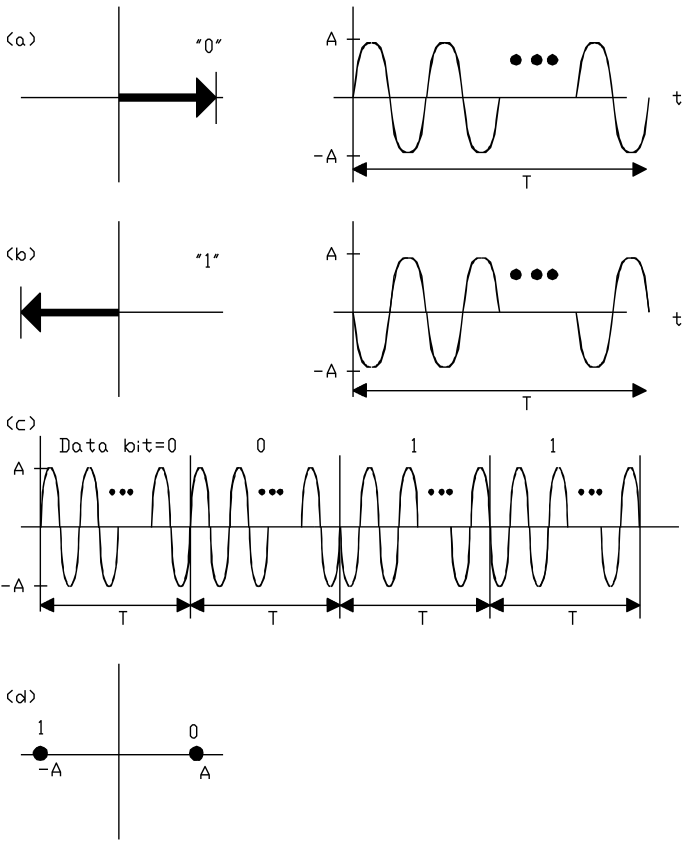
\includegraphics[width=0.55\linewidth]{figs/ch2_secMod_fig1.png}
    \caption{Example of \ac{iq} modulation \cite{Ha2010TheorySystems}}
    \label{fig:ch2_secMod_fig1}
\end{figure}

\par As such, the bits transmitted are represented as positions on an axis of a 2D-space, which is  shown in Figure \ref{fig:ch2_secMod_fig1} (d).

\par Although this figure is just for one of the data signals, \ac{i}, the fact that the quadrature signal \ac{q} is offset $90^{\circ}$ means that it would sit on a perpendicular axis creating a constellation of four symbols as shown in Figure \ref{fig:ch2_secMod_fig2}.

\begin{figure}[H]
    \vspace*{0cm}
    \centering
	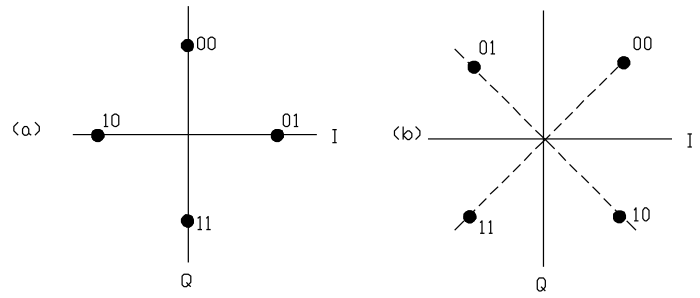
\includegraphics[width=0.5\linewidth]{figs/ch2_secMod_fig2.png}
    \caption{Example for two types of constellation for four symbols \cite{Ha2010TheorySystems}}
    \label{fig:ch2_secMod_fig2}
\end{figure}

\par In Figure \ref{fig:ch2_secMod_fig2}(a) we can observe the simpler case when constellation symbols sit on top of the axes of the graph. This is convenient as the coordinates present us directly with the amplitude for each symbol, but not mandatory. In Figure  \ref{fig:ch2_secMod_fig2}(b), we have the constellation skewed by $45^{\circ}$ and as such the symbols do not lie directly on top of the axes, and the amplitude of each symbol is not directly obtained.

\par More complex \ac{iq} modulation systems may have a multitude of constellations, usually with an amount of symbols that is a multiple of 2. This happens not only because we are modulating using the phase for each symbol but also the amplitude of the signals. As such, we have \ac{qam}.

\section{Phase Shift Arrays}
\label{section:ch2_psa}

\par \ac{psa} are considered a notable advancement in antenna technology. These have greatly influenced modern communications, radar, among several other applications. These are designed to very  carefully manipulate the phase of electromagnetic waves generated on individual elements of the array. This precise control of the phase enables \ac{psa} to use beamforming, beam steering, and adaptive signal processing on their operations to fulfill critical functions and applications.

\par The most relevant characteristic of \ac{psa} is the ability to shift phases. Traditionally, an antenna or array of antennas will receive or transmit a signal. This causes them to have a beam pattern that cannot change their form or direction unless they are moved. However, this does not hold on \ac{psa} that allow for an individual dynamic control of the phase of each antenna element relative to all the other elements. When a change is applied to the phase of these elements, the interaction between the electromagnetic waves also changes, resulting in different interference patterns that can be constructive or destructive in their influence. These can be controlled to achieve the desired characteristics of the beam. There are certain designs of \ac{psa} that can control the amplitude of the waves to shape the interference patterns of the array. There is also another advantage to arrays of antennas that comes in smaller side lobes due to the ability to control the shape of radiation being emitted.

\par The concept of multi-antenna array configurations has existed since the dawn of radio telecommunications, with several elements being synchronized in order to enhance both reception and transmission of radiation. In 1902, Nobel laureate Ferdinand Braun was already successful in transmitting directed wireless telegraph messages using inclined beam antennas \cite{NobelPrize.org2023FerdinandBiographical}.

\par Later advancements were more prominent during the mid-last century as a push towards improving \ac{par} was necessary due to their usefulness during WWI as they were capable of, for example, ground-controlled approach that allowed tracking airplanes and aid traffic controllers to guide pilots during bad visibility conditions.

\par Eventually the advantages of these radar arrays were applied to civilian telecommunications as well. As this happened, there was a shift from fixed antennas to electronically steerable ones. With these, wireless communication systems saw a facilitation in beamforming and beam steering techniques in order to increase efficiency of networks.

\par Nowadays, the evolution of \ac{psa} continues to advance, with the engineering and scientific communities making efforts to reduce both production costs and wasted energy, as well as expanding their range of applications. \ac{psa} have been used on 5G wireless networks, satellite communication systems, or vehicles, as examples.

\par For simplicity, we are going to consider that the distance between every element of the array is going to be constant, and for better performance, a distance of half of the wavelength of the carrier wave.

\subsection{Near Field vs Far Field}
\par The terms Near Field and Far Field serve as indications for the positioning of the \ac{rf} source relating to the \ac{psa}.

\par In Near Field circumstances, our \ac{rf}, from an isotropic antenna, source will be so close to our receiver that the wavefront propagating in front of the array will seem round, or not necessarily perpendicular to all elements of the \ac{psa}. In these situations, the waves arriving at the extremities of the array will be doing so later than they did at the center.

\par Far Field would then be a situation where the \ac{rf} source is positioned in front of the array, but so distant that the wavefront will seem parallel to the \ac{psa}, meaning that it will reach all elements with a delay that can be considered negligible.

\par The criteria adopted to distinguish between these two scenarios are usually described in (\ref{eq:ch2_farfield}). Here, D is the distance between the center of the first element and the last and $\lambda$ is the wavelength of the carrier wave.

\begin{equation}
    \label{eq:ch2_farfield}
    Far Field > 2\cdot\frac{D^{2}}{\lambda}
\end{equation}

\par This equation also allows us to determine that for arrays of small dimensions or for \ac{rf} sources of large wavelengths the distance at which we can consider that we are in Far Field territory is small. On the other hand, for larger arrays or for higher frequencies, the Far Field will happen much further from the \ac{psa}.

\subsection{Beamforming}
\par Beamforming is a technique that has been most useful for telecommunications, specifically for applications on \ac{psa}, as it enables the control of both shape and direction of radiation with precision. As such, performance and specific functionality for several applications is also increased.

\par We can distinguish between two major forms of this technique. There is analog beamforming that through phase shifters or attenuators allows for a less flexible approach. There is also digital beam forming, relying on \ac{dsp} technology to manipulate signals in the digital domain, resulting in more flexible and adaptable implementations, thus being more useful in a wider range of applications.

\subsubsection{Time-Domain Beamforming}
\par For this type of beamforming, the signal being transmitted or received by the array is time delayed or has its phase shifted from antenna to antenna as can be seen in Figure \ref{fig:ch_2_secArray_Array_Time_Delay}.

\begin{figure}[H]
    \vspace*{0cm}
    \centering
    
\includegraphics[width=0.5\linewidth]{figs/ch_2_secArray_Array_Time_Delay.png}
    \caption{Example for Time-Domain beamforming of 4 element array}
    \label{fig:ch_2_secArray_Array_Time_Delay}
\end{figure}

\par For far field applications this means that a wavefront of $45^{\circ}$ inclination will see time delays multiple of $\Delta$t applied at their path in the array, which are then summed together in order to have a more substantial signal at the output of the combining block.

\par The delay considered, $\Delta t$, can be calculated from (\ref{eq:ch2_timedelay}) \cite{Jang2018ABeamformer} where $\lambda$ is considered the wavelength of the carrier wave, $\Psi$ the angle of the beam and c is the speed of light.

\begin{equation}
    \label{eq:ch2_timedelay}
    \Delta t = \frac{\lambda}{2}\cdot\frac{\sin{\Psi}}{c}
\end{equation}

\par It is easily deduced from this equation that for applications where the wavefront is perpendicular to the array, when $\Psi$ is 0, there is no need for any delay, as the result of this equation is also zero, as one may expect. For all other situations where the wavefront and array are not perpendicular, this time delay is needed to achieve the best results possible on the array.

\subsubsection{Phase Shifting Beamforming}
\par This technique is very similar to the previous one, but we express the time delays as phase shifts. Considering that all the antennas in the array are at a distance, \textit{d}, of each other such that $d=\lambda/2$.

\begin{figure}[H]
    \vspace*{0cm}
    \centering
    
\includegraphics[width=0.5\linewidth]{figs/ch_2_secArray_Array_Phase_Shift.png}
    \caption{Example for phase shift beamforming of 4 element array}
    \label{fig:ch_2_secArray_Array_Phase_Shift}
\end{figure}

\par In this situation, $\theta$ is the inclination away from the perpendicular line of the array. Equation (\ref{eq:ch2_phaseshift}) shows how to calculate the phase shift for each element of the array.

\begin{equation}
    \label{eq:ch2_phaseshift}
    \Phi t = \pi\cdot\sin{\theta}\; rad
\end{equation}

\par This simplifies the approach to beamforming by increasing the gain of the captured signal or the transmission of information.

\subsubsection{Digital Beamforming}
\par For \ac{dbf}, the signal being received or transmitted has, at some point, to be converted from analog to digital or digital to analog accordingly. 

\par Figure \ref{fig:ch_2_secArray_DigitalBeamforming} shows an example of a receiver using this technique.

\begin{figure}[H]
    \vspace*{0cm}
    \centering
    
\includegraphics[width=0.5\linewidth]{figs/ch_2_secArray_DigitalBeamforming.png}
    \caption{Example for digital beamforming of 4 element array}
    \label{fig:ch_2_secArray_DigitalBeamforming}https://www.overleaf.com/project/6509e20fd9f6e5936b1c19ab
\end{figure}

\par The most obvious and logical benefit of using \ac{dbf} is that all data is readily available for digital processing, storage, and being worked on without loss to the information \cite{Kasemir2009WidebandBeamforming}. We also have the advantages of a better dynamic range, faster search frame times, and more precise control of both amplitude and phase to reduce sidelobe levels \cite{Skolnik2008RadarHandbook}.

\par One characteristic that cannot be overlooked in order to maintain good performance is the precision and speed of the converters. An optimal \ac{dbf} implementation would have ADCs or DACs with good resolution and fast maximum sampling rate. This would mean that very little to no information about the original data would be lost during the conversion process.

\par These systems, however, typically need a powerful \ac{dsp} or \ac{fpga} in order to process all the information set for transmission or that has been received and also to be able to keep up with the demands that result from the normal operation of the \ac{psa} such as being able to calculate all the variables needed to properly tune each element of the array to maintain proper functioning with the array calibrated to whatever angle needed. 

\par These problems are only exacerbated when high-speed information transfers are the target \cite{Lu2019ApplicationsSystem}, as the system will have to spend more computational resources for all tasks related to signal processing. The same holds true when the number of elements of the array increases, as it will be more taxing for the system to keep every element tuned for the particular situation.

\subsection{Beamwidth and Half-Power Beamwidth}
\par The \ac{ieee} defines beamwidth, or rather \ac{hpbw}, as "In a radiation-pattern cut containing the direction of the maximum of a lobe, the angle between the two directions in which the radiation intensity is one-half the maximum value" and defines the principal \ac{hpbw} as "For a pattern the major lobe of which has a half-power contour that is essentially elliptical, the half-power beamwidths in the two pattern cuts that respectively contain the major and minor axes of the ellipse"\cite{2014IEEEAntennas}.

\par These parameters are more specific to antennas than it is to \ac{psa} itself, but they are also important for the whole array of antennas. 

\par The previous definition regarding beamwidth is the separation in angle units for identical points in opposite sites of the maximum of the pattern. This can be expressed as an approximation in a horizontal coordinate system as shown in Equation (\ref{eq:ch2_beamwidth}) as $\Omega_{A}$.

\begin{equation}
    \label{eq:ch2_beamwidth}
    \Omega_{A} = \theta_{1}\cdot\theta_{2}\; (sr)
\end{equation}

\par In this equation, $\theta_{1}$ represents the azimuth and $ \theta_{2}$ is the elevation on the system used. The notion of depth is not considered, as we are looking only to evaluate the spherical area.

\par \ac{hpbw} is used to measure the angular distance between points of the main lobe of an antenna where the radiation pattern has lost half of its power related to the point of maximum power.

\par Equation (\ref{eq:ch2_hpbwangle}) gives the angle at which point \ac{hpbw} occurs. Equation (\ref{eq:ch2_hpbwsimple}) defines how to calculate \ac{hpbw}.

\begin{equation}
    \label{eq:ch2_hpbwangle}
    \theta  = \arcsin{ \frac{ 0.35 }{\pi }}\cdot\left(\frac{180}{pi}\right)\; (degrees)
\end{equation}

\begin{equation}
    \label{eq:ch2_hpbwsimple}
    HPBW  = 2\cdot\theta(degrees)
\end{equation}

\par Using Equation (\ref{eq:ch2_hpbw}) we can calculate the \ac{hpbw} of a linear and uniform array where N refers to the number of elements in a linear array, $\lambda$ is the wavelength of the carrier wave and $\theta$ is the angle of \ac{hpbw} and d is the distance between elements in this array. The angle $\theta$ refers to the beam angle.

\begin{equation}
    \label{eq:ch2_hpbw}
    \theta_{B}\approx\frac{0.886\lambda}{N\cdot d\cdot\cos{\theta}}
\end{equation}



\par There are also regions of the radiation-pattern that may see null power. Other regions may have less power being radiated through them. The last of these are known as the minor lobes. 

\par All of these characteristics can be observed in Fig. \ref{fig:ch_2_secArray_Beam}. This is a simple representation of a radiation pattern, however, these can be quite complex with several side lobes and multiple nulls.

\begin{figure}[H]
    \vspace*{0cm}
    \centering
    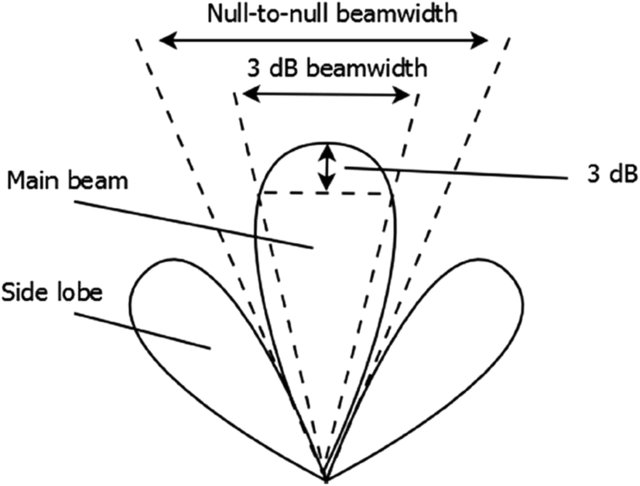
\includegraphics[width=0.5\linewidth]{figs/ch_2_secArray_Beam.jpg}
    \caption{Characteristics of radiation-pattern \cite{Bhattacharyya2020RadiationArrays}}
    \label{fig:ch_2_secArray_Beam}
\end{figure}

\subsection{Antenna Directivity}

\par Antenna directivity is a measurement of a characteristic of an antenna that is compared to an ideal isotropic antenna. This metric is also useful when there is need to evaluate the ability to focus the energy being radiated by the antenna.

\par Directivity is a dimentionless relationship of the antenna's maximum power $P_{MAX}$ and the average power that is radiated in all directions. 

\par For anisotropic antennas, when no direction is given, we consider the direction of maximum radiation intensity \cite{ConstantineA.Balanis2016AntennaDesign}. Equation (\ref{eq:ch2_maxdirectivity}) helps define this parameter, where $D_{0}$ is the maximum directivity, $U_{MAX}\;(W\cdot sr)$ is the maximum radiation intensity and $P_{RAD}\;(W)$ is the total radiated power of the antenna.

\begin{equation}
    \label{eq:ch2_maxdirectivity}
    D_{0}=\frac{4\cdot\pi\cdot U_{MAX}}{P_{RAD}}
\end{equation}

\par When an antenna has orthogonal polarization components, \citeauthor{ConstantineA.Balanis2016AntennaDesign} defines $D_{0}$ for a spherical coordinate systemn as shown in equation (\ref{eq:ch2_orthodirectivity}).

\begin{equation}
    \label{eq:ch2_orthodirectivity}
    D_{0}=D_{\theta}+D_{\phi}
\end{equation}

\par Here, the components for the partial directivies $D_{\theta}$ and $D_{\phi}$ are defined in (\ref{eq:ch2_orthodirectivitytheta}) and (\ref{eq:ch2_orthodirectivityphi}) respectively for each of the orthogonal field components.

\begin{align}
    D_{\theta} &= \frac{4\cdot\pi\cdot  U_{\theta}}{(P_{RAD})_{\theta}+(P_{RAD})_{\phi}}
    \label{eq:ch2_orthodirectivitytheta} \\
    D_{\phi} &= \frac{4\cdot\pi\cdot  U_{\phi}}{(P_{RAD})_{\theta}+(P_{RAD})_{\phi}}
    \label{eq:ch2_orthodirectivityphi}
\end{align}

\subsection{Antenna Gain}
This is a metric typically used to describe the gain of the antenna in a given direction. It evaluates the efficiency of the antenna with its directivity. It is described in Equation \ref{eq:ch2_antennagain}

\begin{equation}
    \label{eq:ch2_antennagain}
    G =  \frac{P_{RAD}}{P_{INPUT}}\cdot D_{0}
\end{equation}

\par Here, $P_{RAD}$ is the total amount of radiation power that the antenna is capable of outputting when a certain power, $P_{INPUT}$, is being supplied.

\subsection{Aperture}
\par Maximum effective aperture evaluates how well an antenna can receive radiation and the wavelength of the electromagnetic wave. The effective aperture for antenna, $A_{E}$, can be calculated using Equation (\ref{eq:ch2_antennaaperture}) \cite{Delos2020PhasedFactor}. Typically, this parameter is used on the direction of maximum radiation intensity \cite{ConstantineA.Balanis2016AntennaDesign}.

\begin{equation}
    \label{eq:ch2_antennaaperture}
    A_{E} = \frac{G\cdot \lambda^{2}}{4\cdot\pi}
\end{equation}


\subsection{Array Factor}
\par \ac{af} is a metric used to express the combined radiation pattern of the eletctromagnetic contributions of all individual elements in a matrix. By helping to understand how all individual radiating elements in the array interact with each other and, as a whole, generate the radiation pattern of the array, \ac{af} is one useful tool in the process of optimizing the performance of the array for the specific application that it is designed to accomplish.

\par This function depends on the position of each antenna element of the matrix, the phase and amplitude of their respective electromagnetic fields relative to other elements in the matrix and certain characteristics specific to the antennas themselves.

\par This means that each array, due to all the possibilities within these parameters, has a specific \ac{af} of its own. As there is no dependency of the \ac{af} with the directional characteristics of the antennas \cite{ConstantineA.Balanis2016AntennaDesign}, we can simplify the calculation process by considering each antenna in the array as isotropic. In this way, \citeauthor{ConstantineA.Balanis2016AntennaDesign} defines the total field of an array as in Equation (\ref{ch2_totalfieldarray}).

\begin{equation}
    \label{ch2_totalfieldarray}
    E_{TOTAL} = E_{element}\cdot AF(\theta)
\end{equation}

\par The value for \ac{af} for the center of the array is given by Equation (\ref{ch2_arrayfactor})\cite{Delos2020PhasedFactor}.

\begin{equation}
    \label{ch2_arrayfactor}
    AF(\theta) = \frac{\sin(\frac{N}{2}\cdot\Psi)}{\sin(\frac{N}{2}\cdot\Psi)}
\end{equation}

\par Here, $\Psi$ represents the phase difference from the previous element of the array, and N is the total number of elements in the array.

\subsection{Grating Lobes}
\par Grating lobes are secondary radiation lobes that are observed when, in antenna arrays, the distance between the radiating elements of the array is less than half of the desired wavelength of the array. They are taken into consideration in those conditions as they appear due to the periodicity of antenna arrays. These can be harmful to the overall operation of the array.

\par These can cause interference in communication systems with nearby sections of the electromagnetic spectrum and disrupt the performance of the array, leading to a loss in directivity or the ability of the antenna array to focus its beam.

\par Figure \ref{fig:ch2_secArray_GratingLobes.png} shows how a different spacing on 32 elements of an array, despite not necessarily decreasing the intensity of the main lobe, significantly changes the format of the radiation-pattern and demonstrates the existence of a now new lobe when the phase of the array is shifted.

\begin{figure}[H]
    \vspace*{0cm}
    \centering
    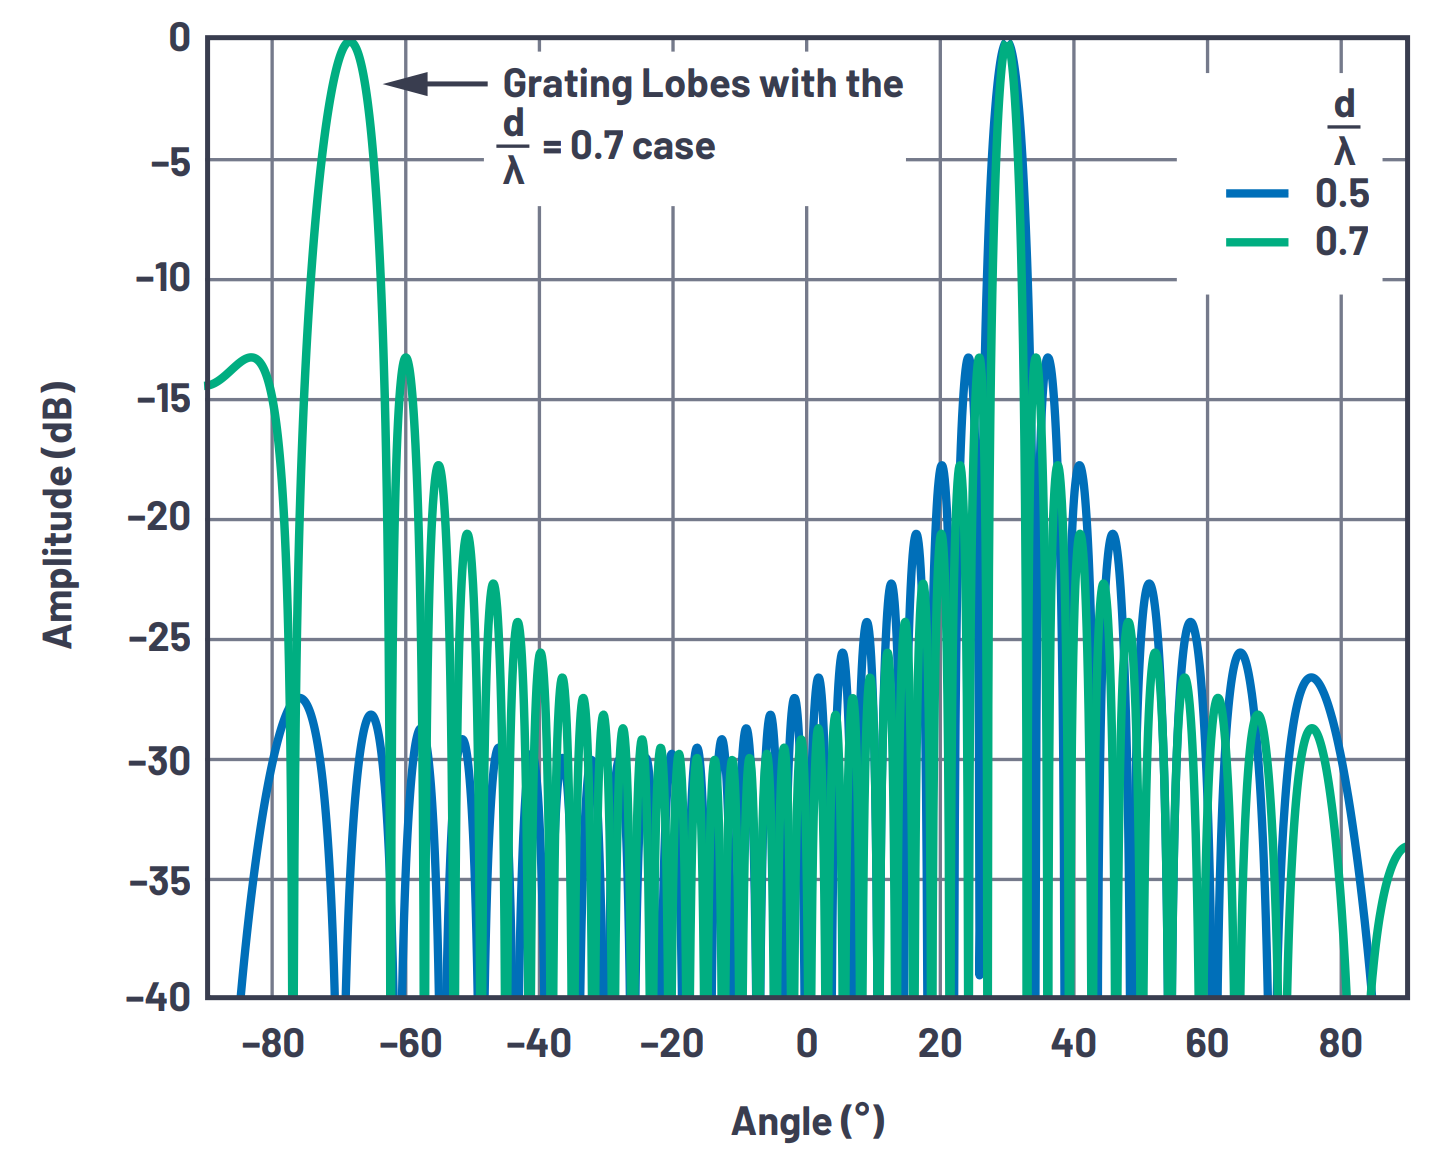
\includegraphics[width=0.5\linewidth]{figs/ch2_secArray_GratingLobes.png}
    \caption{Grating Lobes for 32 element array \cite{Delos2020PhasedTapering}}
    \label{fig:ch2_secArray_GratingLobes.png}
\end{figure}


\par According to \citeauthor{Delos2020PhasedTapering}, we can obtain at what beam angle we obtain grating lobes if we consider the solutions of (\ref{ch2_gratinglobes}).

\begin{equation}
    \label{ch2_gratinglobes}
    \theta = \arcsin{\left(\frac{\lambda}{d}\cdot \left( m + \frac{d\cdot\sin{\theta}}{\lambda} \right)\right)}
\end{equation}

\par Here, \textit{d} is the distance between elements, $\lambda$ the wavelength of the carrier and \textit{m} is all possible spatial images for the appearance of a periodic replica. The value of \textit{m} can be any possibility within the sequence $m = \pm1, \pm2, etc$.

\par When the solution of the equation is a single real number, we are able to avoid its presence, which means that for $m\geq1$ Equation (\ref{ch2_gratinglobescondition}) must be true.

\begin{equation}
    \label{ch2_gratinglobescondition}
    1 < \left|\frac{\lambda}{d}\cdot \left( m + \frac{d\cdot\sin{\theta}}{\lambda} \right)\right|
\end{equation}

\par When this relation is not met for $m > 0$, then $\arcsin$ returns a real number that results in a grating lobe. If the solution is otherwise an imaginary number, then it can be ignored. 

\subsection{Spacing between radiating elements}
\par We know that when distance for ajdacent antennas in the array is $\lambda/2$ there is not interference between the radiation of neighboring elements. However, for distances above $\lambda/2$ there is a risk that grating lobes appear causing problems on the array's behavior due to spacial aliasing, and we can use the Nyquist theorem in this context \cite{Delos2020PhasedSquint}. 

\par This parameter should be considered when designing the array, as it may come as a trade-off between the size of the array, the size of the scanning angle, operating frequency, and the occurrence of these undesirable phenomena.

\subsection{Mutual Coupling}
\par In \ac{psa}, each radiating element can be influenced by and influence its neighbouring elements. This can introduce challenges that limit the performance of the system. Each element's performance changes depending on how closely or sparsely they are from one another in the array, for example. But there can be other factors that can cause mutual coupling, other than the simple geometric position of the radiating elements of the array. Operating frequency, due to the size of the wavelengths being considered, the steering of the radiation-pattern and the presence of conducting materials in the \ac{psa}.

\par Also, not all elements will suffer from mutual coupling to the same extent. One can see that in a square array of $N\times N$ elements, the ones on the corners will have fewer surrounding neighbors, followed by all the other ones on the edges, and as we reach closer to the center of the array, this effect might keep changing. 

\subsection{Beam Angle Resolution}
\par As seen previously, these devices can be controlled by timed delay or phase shift. These do not produce continuous intervals of numbers. Most have a maximum resolution that they can work with. They exist in discrete domains where both time and phase intervals have steps. And this problem is insensitive to whether the system is being controlled via an analog signal or digitally.

\par For analog systems, this is a very straightforward process. A small amount of voltage or current will increase the time delay or phase shift by a certain amount. But for digitally controlled systems we have to wonder how many bits do we need to change the time delay or phase shift.

\par For cases where a phase shifter is used, the resolution of the \ac{psa} will differ from the resolution of the phase shift used, as expected. Equation (\ref{ch2_angleLSB}) establishes the relationship between the number of bits, B, of the phase shifter and its angle resolution.

\begin{equation}
    \label{ch2_angleLSB}
    \Phi_{LSB} = \frac{\pi}{2^{B}}
\end{equation}

\par If we consider Equation (\ref{ch2_gratinglobes}) seen previously, for a linear array of \textit{N} elements spaced by half a wavelength, we obtain an angle resolution $\theta_{R}$ in relation to the angle resolution in bits, $\Phi_{LSB}$, as shown in Equation (\ref{ch2_beamResLSB}).

\begin{equation}
    \label{ch2_beamResLSB}
    \theta_{R}\approx\arcsin{\frac{\Phi_{LSB}}{N\cdot\pi}} \text{\cite{Delos2020PhasedDevicesc}}
\end{equation}

\par Figure \ref{fig:ch_2_secArray_PhaseResElements.png} details how Equation (\ref{ch2_beamResLSB}) expresses the resolution of the beam angle with the total number of elements in a linear array spaced by half of a wavelength according for different phase shifters with different $\Phi_{LSB}$. In this Figure, it can be seen that for phase shifters with only two bits, as blue, the resolution is worse than for the case when the phase shifter has 4 bits, seen in purple, for example.
\begin{figure}[H]
    \vspace*{0cm}
    \centering
    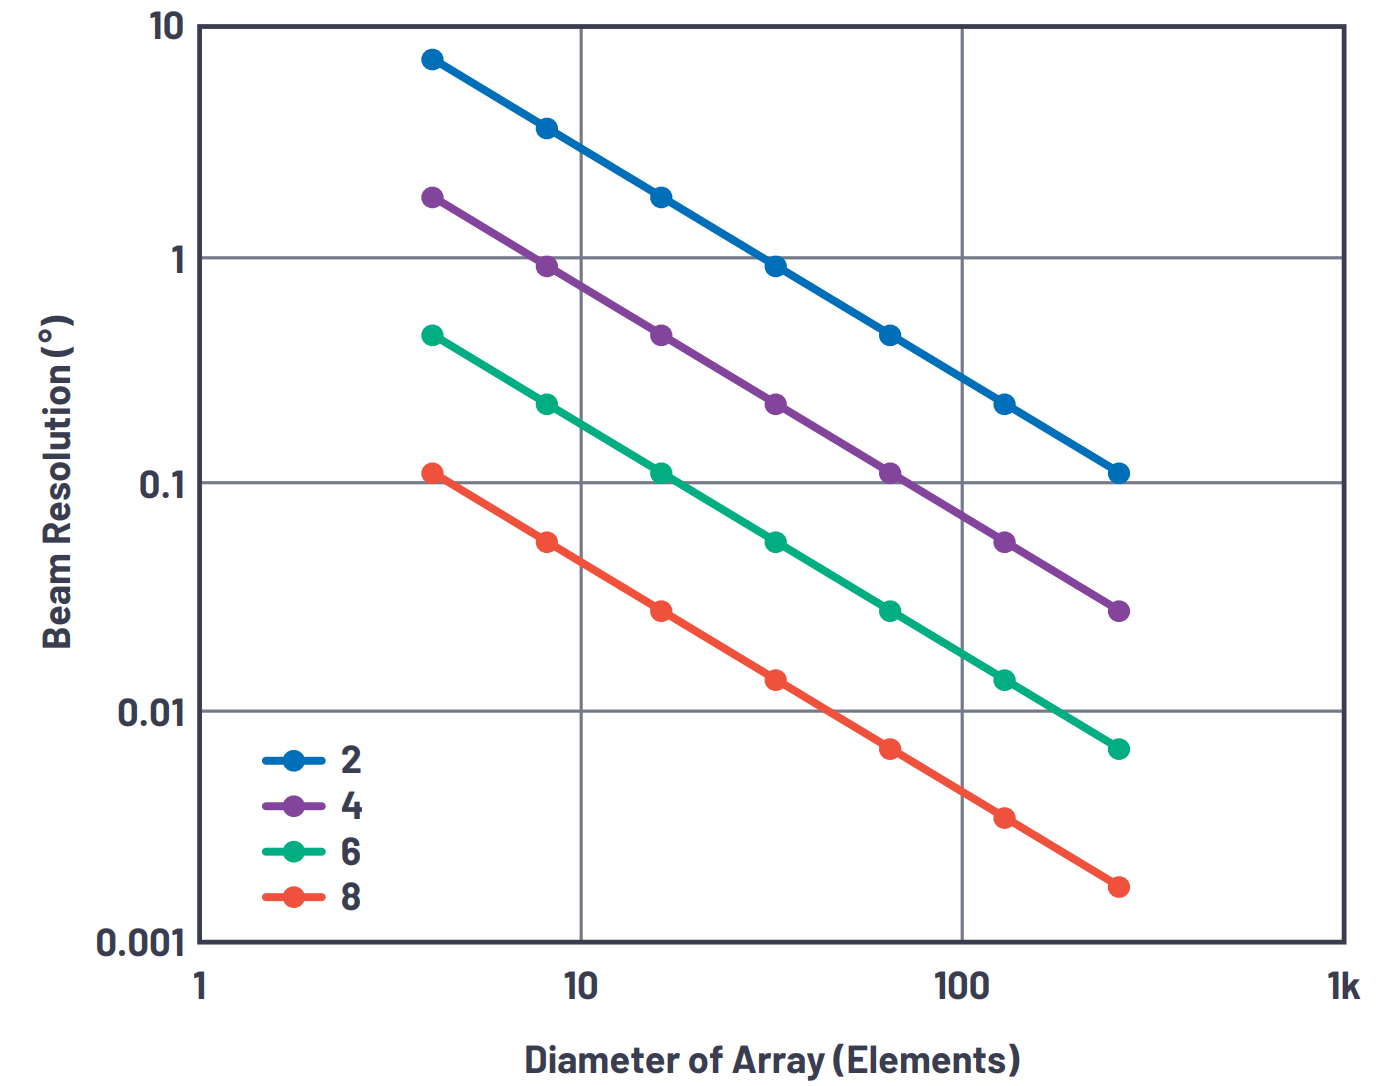
\includegraphics[width=0.5\linewidth]{figs/ch_2_secArray_PhaseResElements.png}
    \caption{Beam angle resolution relation with the array number of elements for various phase shift resolution\cite{Delos2020PhasedDevicesc}}
    \label{fig:ch_2_secArray_PhaseResElements.png}
\end{figure}

\par This helps to visualize how the bit resolution of the phase shifter can influence the total amount of beam angle resolution of the array. It also demonstrates the importance of choosing the right phase shifter with and appropriate $\Phi_{LSB}$ for what is expected of the \ac{psa} that is being designed. As expected, the smaller $\Phi_{LSB}$ is then the better is the beam resolution of the array. This is particularly important for systems that have a small number of elements, or we may see that beam resolution may negatively affected the whole operation of the system, providing poor beamforming capabilities.

\par However, even a phase shifter with a $\Phi_{LSB} = 90^{\circ}$, which means two bits total, can achieve a small beam resolution for arrays with large numbers of elements.

\subsection{Quantization of Sidelobes}
\par Phase shifters with larger $\Phi_{LSB}$ resolutions tend to be a hindrance to system gain.
\par \citeauthor{Skolnik2008RadarHandbook} explains that the relation between the total number of bits, \textit{B}, of a phase shifter and the loss in gain of the system is defined in Equation (\ref{ch2_GainLossLSB}).

\begin{equation}
    \label{ch2_GainLossLSB}
    \Delta G = \frac{\pi^{2}}{2^{2\cdot B}\cdot 3}
\end{equation}

\par The energy lost due to this effect is then divided along the side lobes of the system. It is easy to deduce that for systems where the phase shifter has a larger $\Phi_{LSB}$ resolution, the total loss in gain will be larger than if the \ac{psa} had a phase shifter with a small $\Phi_{LSB}$.

\par Figure \ref{fig:ch_2_secArray_QSLL.png} shows a visual representation of how the \ac{qsll}, in $\:\si{dB}$, relates to the number of bits of the phase shifter. 

\begin{figure}[H]
    \vspace*{0cm}
    \centering
    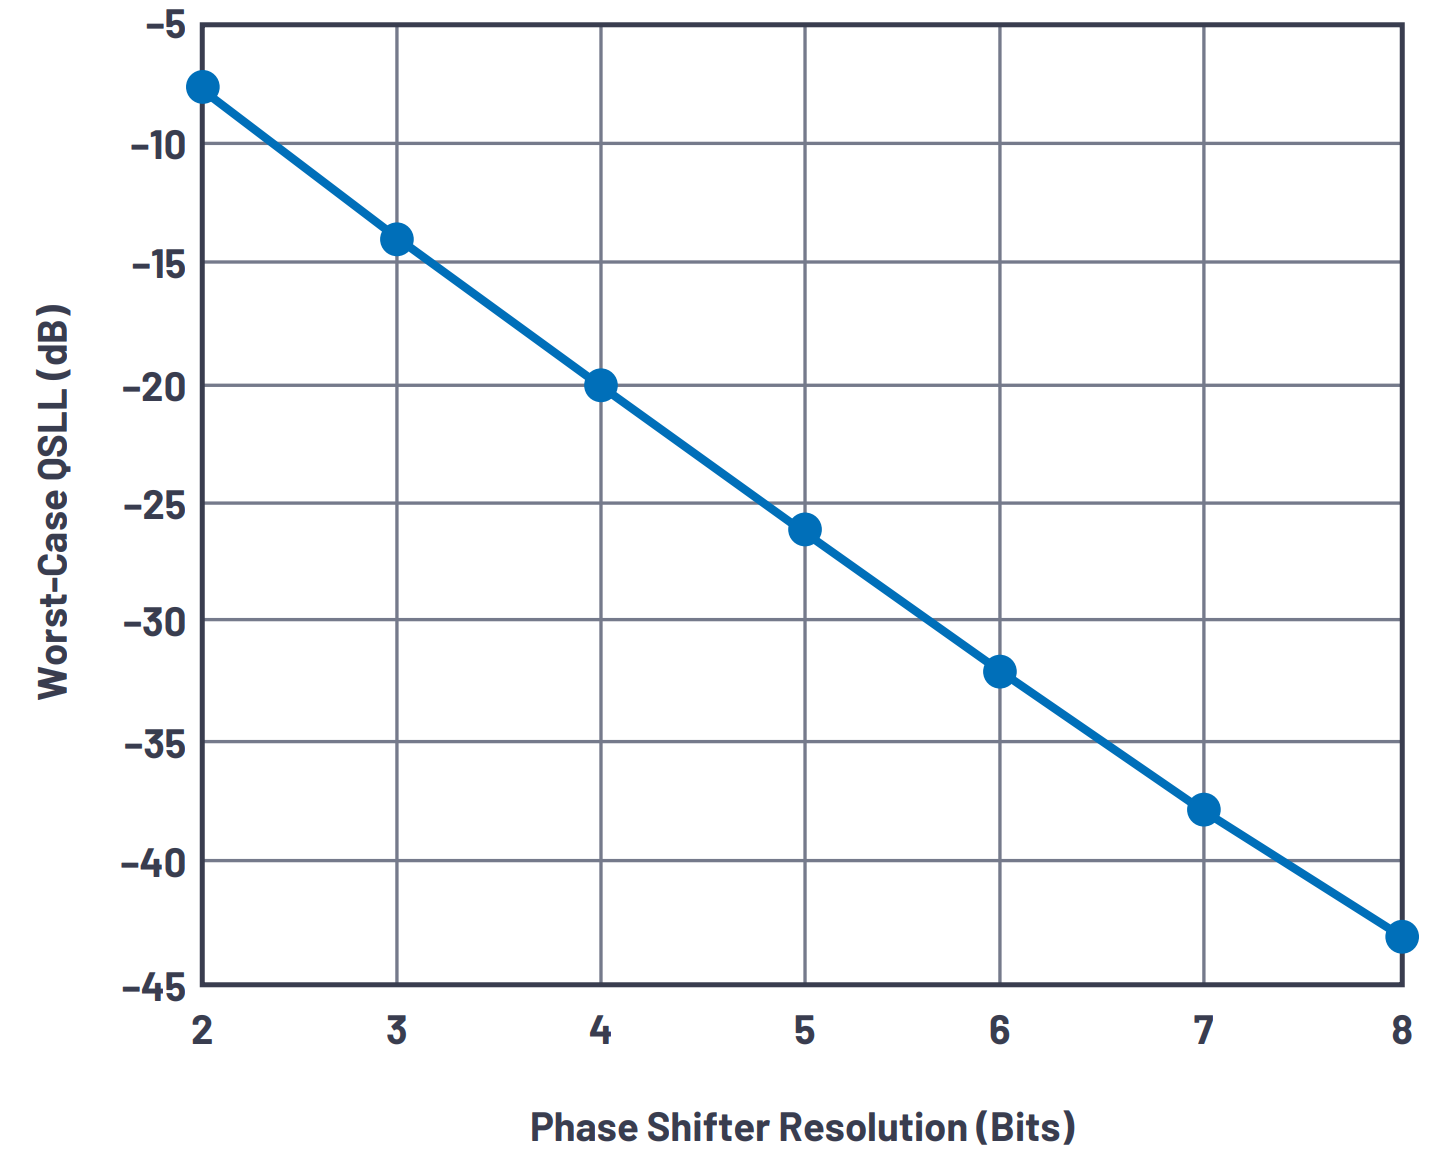
\includegraphics[width=0.5\linewidth]{figs/ch_2_secArray_QSLL.png}
    \caption{Quantization sidelobe levels relation with phase shifter resolution\cite{Delos2020PhasedDevicesc}}
    \label{fig:ch_2_secArray_QSLL.png}
\end{figure}

\subsection{Application of Phase Shift Arrays Nowadays}
\par These systems are extremely attractive in the realm of radar systems. From being used in armed forces all over the world to weather forecasting, air traffic control, and space exploration, they can be used due to their ability in manipulating the shape, angle, and directivity of their radiation-patterns, how easy it is to implement adaptive interference cancelation algorithms due to the number of antennas used, and good performance at tracking and distinguish signals.

\par They are a foundational equipment in telecommunication systems, due to their ability to beamform and allowing for beamsteering of the radiation pattern.

\par With the advent of 5G technology and the massive \ac{mimo} systems that come with, \ac{psa} have a pivotal role in the delivery of high-speed and low-latency communications that these modern applications require. The fact that many beams can be controlled on a one-to-one level is one big selling point for this field. 

\par \ac{psa} have also been used in the medical field, their implementation greatly benefiting the advances in medical imaging such as ultrasound and magnetic resonance imaging examination techniques. The enhanced resolution and overall quality of the images that are obtained, along with the ability to direct very precisely the radiation-patterns allows for more accurate diagnoses without the need for more invasive methods of the past, such as exploratory surgery.

\par Their use has also been helping physics and astronomers alike in the exploration of the universe because of their capabilities regarding beam steering that allows the study of specific regions or celestial objects.

\subsection{Benefits and Disadvantages of \ac{psa}}
\par In this section, the main identified advantages and disadvantages are outlined in the following paragraphs. 

\subsubsection{Advantages}
\par Easily the very first benefit that comes to mind for \ac{psa} is the exceptional and reliable ability to steer electromagnetic beams with very good precision. As such, all applications that benefit from beamstearing like tracking, reduced interference, and fine-tuned signal reception, can only be empowered by their use.

\par The enhanced efficiency of \ac{psa} is also to be noted here, as they can precisely concentrate energy where it is needed and minimize signal loss and interference that can result in higher data transfer rates and extended ranges.

\par As seen previously, \ac{psa} can be highly versatile with their use in various scientific fields, each with different operating frequencies and requirements.

\par The fact that they can be controlled electronically, instead of being fixed or relying on mechanical motors, allows swift adjustments to the direction of their beams and also their shape to better respond to the need of their application.

\subsubsection{Disadvantages}
\par High performance \ac{psa} can be costly. The development, deployment and maintenance of these systems, with specialized materials, components, and manufacturing processes, can contribute to an elevated cost that limits its accessibility for smaller-scale applications, although there have been efforts to integrate them as \ac{mmic}.

\par Another point of concern for \ac{psa} is their complexity. Both in design and operation, these are very complex pieces of technology that require an understanding of electromagnetic fields, some signal processing both for digital and analogue scenarios, and knowledge in control systems. This poses a challenge in terms of calibration and troubleshooting that requires skilled engineers and technicians to maintain proper operation.

\par Unfortunatly, \ac{psa} may require a substantial amount of electrical resources to remain operational. This restricts their usage in battery-powered devices or low-power applications.

\par Due to the large number of electronic components in a \ac{psa}, they can be susceptible to electromagnetic interference from external sources, which may hinder their deployment for certain applications where this factor could be a concern.

\section{\acl{mimo} Systems}
\par \ac{mimo} technology has been a cutting-edge development in wireless communications with a lot of focus on investigation and improvement over the last years \cite{Spencer2004AnDownlink}. With advancements in antenna arrays for both transmitter and receiver, helping to enhance the transmission of data over distance, allowing for bigger throughput and the system's performance \cite{Spencer2004AnDownlink}\cite{Alexandropoulos2022Full-DuplexDirections}\cite{Zhang2006FutureNetworks}.

\par \ac{mimo} technology emerged as a solution to the challenges wireless communication systems have been facing\cite{Spencer2004AnDownlink}. Typical wireless systems as we know them have faced problems with radio frequency spectrum limitations, with every frequency band being costly, multipath distortion that can be due to a variety of reasons, and interference \cite{Spencer2004AnDownlink}\cite{Lawton2008IsCommunications}. With data consumption continuously growing exponentially, and with no expectation for a decline in the near future due to the proliferation of smart devices, more streaming platforms that can range from normal media formats to cloud video gaming, \ac{iot} devices and applications, there has been an increased demand for higher data rates, with little to no dropped information, enhancing the networking capacity in order to provide a consistent quality service to all clients \cite{Spencer2004AnDownlink}.

\par \ac{mimo} technology then came as a technology that could address these constraints and overcome them. With the aid of sophisticated algorithms and antenna arrays, \ac{mimo} systems can simultaneously transmit and receive various data signals over the same radio channel \cite{Alexandropoulos2022Full-DuplexDirections}\cite{Zhang2006FutureNetworks}. This type of multiplexing is done by sending data over multiple paths, taking advantage of what conventional radio systems consider interference and fading \cite{Spencer2004AnDownlink}\cite{Alexandropoulos2022Full-DuplexDirections}. This effectively provides a significant boost to the system capacity and efficiency without the need for additional bandwidth or increase in transmission power needed for wireless communication \cite{Lawton2008IsCommunications}.

\par The flexibility and adaptability of these systems that, operating on the physical layer, can seamlessly integrate with several types of wireless transmission protocols, including the widely available and used Wi-Fi IEEE 802.11 standards \cite{Spencer2004AnDownlink}\cite{Lawton2008IsCommunications}.

\par Although \ac{mimo} technology has been developed to enhance wireless communications, it is not perfect: Energy consumption, financial cost, and competition from other parallel communication technologies may become hindrances in \ac{mimo} future development \cite{Rusek2013ScalingArrays}. However, the \ac{mimo} technology has been allowed a solid foothold with its integration into emerging broadband standards \cite{Zhang2006FutureNetworks}. This becomes more evident as major companies invest on the development of this technology with \ac{mimo}-based products.

\par There have been plans for the future development of large \ac{mimo} systems with a greater amount of antenna elements have been proposed than in today's setups, with the aim of being more efficient \cite{Zhang2006FutureNetworks}. Also, it is important to consider that the robustness of these systems also has room to improve. As systems grow in both scale and requirements, new implications in \ac{dsp}, programming, and network design are revealed \cite{Zhang2006FutureNetworks}. 

\subsection{Principles and Operations}
\par \ac{mimo} leverage the spatial dimension to improve the performance of the system. 

\subsubsection{Space-Time Modulation and Coding}
\par Unlike \ac{siso} systems, \ac{mimo} technology relationship between input and output cannot be described as if it were a scalar, rather they are described as a vector, for example $y=Hx+n$. The extension of space, by using several antenna elements, and time, with different symbol times, is commonly known as space-time coding \cite{Goldsmith2005WirelessCommunications}.

\par This technique allows for an easier way of understanding and implementing an algorithm where, with $M_{T}$ the number of antenna elements transmitting, $M_{R}$ the total number of antenna elements at the receiver and T the symbol times, we can express the input matrix as $X=[x_{1},...,x_{T}]$ for the input channel $M_{T}\times T$ and the channel output matrix for $M_{R}\times T$ expressed as $Y=[y_{1},...,y_{T}]$. We can also now add the noise that is captured by the receiver as $N=[n_{1},...n_{T}]$. The model that we arrive at can be described as shown in Equation (\ref{ch2_MatrixMIMO}) according to \citeauthor{Goldsmith2005WirelessCommunications}.

\begin{equation}
    \label{ch2_MatrixMIMO}
    Y=HX+N
\end{equation}

\subsubsection{Spatial Multiplexing}
\par One of the techniques used by multi-antenna arrays in \ac{mimo} technologies for smaller frequency bands consists of spatial multiplexing systems. This requires that the receiver end be able to demultiplex the transmitted information.

\par In a system described by the model suggested in Equation (\ref{ch2_MatrixMIMO}), the overall channel capacity, $C_{SM}$ is described by Equation (\ref{ch2_ChannelCapacity}).

\begin{equation}
    \label{ch2_ChannelCapacity}
    C_{SM} = \sum_{i=1}^{r} \log_2\left( 1+ \frac{\rho}{M_{T}}\cdot\lambda_{i}\right)
\end{equation}

\par Here, $\rho$ represents the signal-to-noise ratio, $\lambda_{i}$ is the i-th eigenvalue of the matrix $HH^{H}$ and r is the rank of this matrix\cite{Kalachikov2018PerformanceModels}.

\par In order for a receiver to distinguish one data stream from the interference of the other $M_{T}-1$ that are being transmitted, algorithms such as \ac{mmse} and \ac{zf} can be used.

\par For system using \ac{zf}, we can use the \ac{zf} equalizer $W_{ZF}$ shown in Equation (\ref{ch2_zfequal}) on the received data Y, in this case a vector, to retrieve the vector $x_{ZF}$ we are interested in shown in Equation (\ref{ch2_zfequal}) \cite{Mehana2012DiversityReceivers}. 

\begin{equation}
    \label{ch2_zfequal}
    W_{ZF} = (H^{H}H)^{-1}H^{H}
\end{equation}

\begin{equation}
    \label{ch2_zfequal}
    x_{ZF} = W_{ZF}y
\end{equation}

\par This technique can, however, lead to noise amplification problems. Therefore, this requires a \ac{mmse} equalizer to reduce this effect. Note that this also involves a more complex implementation. The output of this detector will then be as described by Equation (\ref{ch2_mmseequal}) where $\sigma$ is the known standard deviation of the noise present in the receiver\cite{Kalachikov2018PerformanceModels}.

\begin{equation}
    \label{ch2_mmseequal}
    x_{ZF} = (H^{T}H+\sigma^{2}I)^{-1}H^{T}y
\end{equation}

\subsubsection{Spatial Diversity}
\par Spatial diversity consists of employing several transmitters and receivers to provide some level of fading compensation. This also helps prevent situations where the signal is blocked due to some accidental obstacle in its way\cite{Navidpour2007BERDiversity}. 

\par This technique maintains high transmission rates when the number of antenna elements in the receiver is equal to the number of the transmitter. It is undesirable for number of elements of the receiver is larger than the number in the transmitter \cite{Bharati2020RealizationGains}.

\subsubsection{Channels}
\par In the model presented for \ac{mimo} systems, the matrix $H$ is used to represent the channel between the transmitter and the receiver. Characterizes the scattering of the propagation environment between multiple antennas at both ends of the channels. This matrix contains the relationships between the transmitter's and the receiver's antenna elements.

\par The channels characteristics have a profound impact on how signals are received and what decoding strategies must be used to establish proper communication, for example, based on the speed at which signals fade.

\subsubsection{\acl{snr} and \acl{sinr}}
\par Systems like that use \ac{mimo} technology suffer from what is known as \ac{sinr}. This metric establishes a relationship that also includes the effect of each channel being transmitted on the other channels present, unlike \ac{snr} that only takes into account the effects of noise present on the channel of interest.

\par If we consider $P_{R}$ the power of the channel's signal that is received, $N_{0}$ the noise power spectral 
density, $B$ the bandwidth of the channel and $P_{I}$ the power caused by interference of all the other channels, then Equation (\ref{ch2_sinr}) will define the total \ac{sinr} present.

\begin{equation}
    \label{ch2_sinr}
    SNIR = \frac{P_{R}}{N_{0}\cdot B + P_{I}}
\end{equation}

\par For \ac{snr} we do not consider $P_{I}$ as in Equation (\ref{ch2_snr}). This metric is then less useful when working with \ac{mimo} systems.

\begin{equation}
    \label{ch2_snr}
    SNIR = \frac{P_{R}}{N_{0}\cdot B}
\end{equation}

\par If \ac{sinr} is high, then this means that our system still has room for a larger channel capacity, as we still have not yet approached a situation where the interference caused by neighboring channels hinders the overall system performance.

\subsubsection{Rayleigh and Rician Channel Models}
\par Both these models help describe the environment in which the signals are transmitted. They are crucial in simulating and describing system performance for different conditions.

\par Rayleigh channel model was developed to be used in systems where there is no \ac{los} between the transmitter and receiver ends of the channel. This can be, for example, in applications where there are obstructions in between them, such as in cities with urban areas. The main characteristic of this channel is its lack of a dominant component.

\par The Rician channel model describes situations where there is a \ac{los} between the transmitter and the receiver and as such it considers the presence of a direct component as well as scattered components.

\subsubsection{\acl{sumimo}}
\par This technique makes it so that all of the antennas in an array for a \ac{mimo} system are used on a single user. This way, the user's data stream will be split over the various elements in the array, forming multiple streams of data. By doing this, we can significantly increase the throughput for that user.

\par This is a simple method to implement as there is no need to deal with multiple users.

\subsubsection{\acl{mumimo}}
\par Contrary to \ac{sumimo}, this technique deals with the scenario where a multitude of users share the same \ac{mimo} system, and instead all active users must share the antennas in the arrays. In this way, the antennas will transmit and receive data from multiple users simultaneously.

\par This greatly limits the throughput for each user, but will help to improve the user experience as there will be room to accommodate all the users at the same time meaning that the delay that each user faces is reduced. These systems are highly adaptable and capable of allocating resources based on their total usage. If there are less users actively needing to transmit or receive data, then the resource pool is divided between those who need it.

\par These systems are, however, more complex than the previous ones. This implies that sophisticated \ac{dsp} techniques may be needed to enable the system to do its job.

\subsubsection{\acl{mmimo}}
\par This is the expansion of the previous system. These systems are a key component for 5G applications. The massive portion of the name comes from the fact that these system could use arrays with up to hundreds of antennas, and serve many users on a dense area. Base stations for these systems may reach even larger proportions. For \acl{mmimo} systems, the large number of antennas helps to focus the energy of antennas into very specific regions of space, allowing for efficient use of the spectrum frequency. This improvement in spectral efficiency helps to increase the capacity of the whole system.

\par The fact that the number of antennas is so large also helps to improve the quality of the signal being delivered, reducing reliability problems that could otherwise be felt.

\par With proper direction towards users, the energy efficiency of these systems can also be increased, reducing overall energy consumption.

\par Much like \ac{mumimo} systems, the complexity increases. These systems require an even more complex \ac{dsp} technique, and usually require precise hardware calibration and maintenance of the large number of antennas in the arrays used.

\par This is, however, the future of \ac{mimo} systems. These are incredibly useful in the present society with cities becoming more densely populated, and users requiring faster response times and larger throughput technologies to satisfy their necessities and desires. 

\subsubsection{\ac{mimo} in Modern Wireless Standards}
\par The applications of \ac{mimo} systems are vast. Consumer electronics, for instance, have been benefited greatly by them in the past years. A quick search on Intel's website shows that there are at least 126 different products where \ac{mimo} technologies were applied.

\par With the introduction of the IEEE 802.11n-2009 norm, came the first standard for \ac{sumimo} technologies to be used on Wi-Fi systems. For 802.11n systems, this meant that those who use \ac{mimo} technologies, the user benefits from higher theoretical speeds.

\par For instance, for home networks, the fact that \ac{mimo} uses multipath to operate, the information being transmitted to and from the \ac{ap} can freely bounce off surfaces, obstacles, etc. and still the interference caused by this is almost negligible.

\par These systems also benefit from an increased number of antennas. For an \ac{ap}  with at least 3 antennas, the connections established achieve speeds of 600 Mbps, whereas for 2 antennas we may see this connection speed halved to 300 Mbps.

\par Norm IEEE 802.11ac-2013 introduced \ac{mumimo} operation with 8 spatial streams for \ac{ap}s. For example, one \ac{ap} equipped with 4 antennas can transmit one stream of data to four users, one stream per antenna. This specification helped raise the throughput for each user by around 2.5 times, while reducing latency per user and increasing the spectral efficiency of the system.

\par This last characteristic is particularly important in densely packed areas such as apartment buildings, offices, etc. where there may be many devices that need to be transmitting or receiving at the same time. As such, each band of the spectrum becomes more valuable.

\par Future plans have been made for the IEEE 802.11be norm, which is expected to use 16 spatial streams, and a maximum theoretical throughput of 30 Gbps. These advancements in technology are considerable, as these equipments will be capable of speeds much higher than those that Internet Service Providers are effectively able to provide most costumers with. In Portugal, NET.mede, a service provided by ANACOM, estimates that more than half of the population has access to internet slower than 100 Mbps, as seen in the graphs of Figure \ref{fig:ch_2_netmed.png} \cite{ANACOM2023EstastisticasNET.mede}.

\begin{figure}[H]
    \vspace*{0cm}
    \centering
    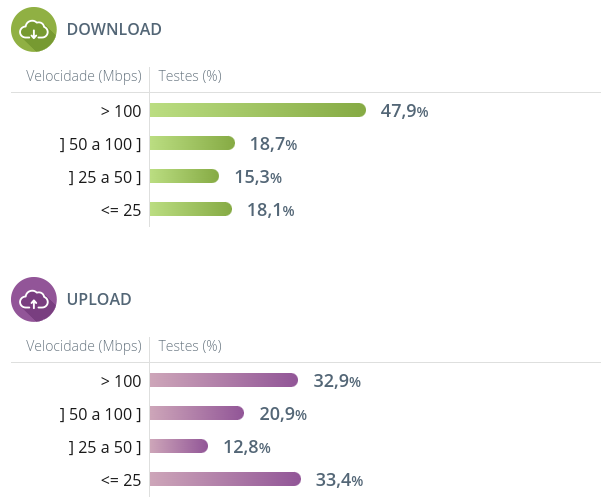
\includegraphics[width=0.5\linewidth]{figs/ch_2_netmed.png}
    \caption{Internet speed distribuition in Portugal\cite{ANACOM2023EstastisticasNET.mede}}
    \label{fig:ch_2_netmed.png}
\end{figure}

\subsubsection{Channel Estimation}
\par In wireless communications systems, the transmitted signals will be affected by various channel impairments. To efficiently decode received signals in \ac{mimo} systems, receivers must have knowledge of the channel through which the data have been propagated. This is usually done by channel estimation techniques.

\par For Pilot-Based Channel Estimation, the transmitter will send known signals, pilots, along with the data that is being transmitted. The receiver will then compare the signals it receives with what was expected for the signal to look like. This way, it can determine the channel's characteristics. The simplicity of this approach makes it the most common approach to determine the characteristics of the channel.

\par Blind Channel Estimation, as the name implies, relies only on the information it receives, without the presence of any pilots. It then performs a statistical analysis of the signals received in order to estimate the properties of the channel. The fact that this method does not have to send any pilot means that it can become more bandwidth-efficient, but will overall be more complex and difficult to implement than pilot-based channel estimation.

\par Semi-Blind Channel Estimation is a method that combines both blind and pilot based channel estimation. This method is the most attractive for use in \ac{mumimo} and \ac{mmimo} systems. This technique relies on knowledge of past experiments (training information) for the blind part and data symbols for the pilot-based approach. This helps to reduce the contamination of the bandwidth with unnecessary pilots, while being less complex and based on pure blind channel estimation\cite{Nayebi2018Semi-blindSystems}.

\subsubsection{Interference Cancellation}
\par Interference is one of the major challenges wireless communications can face. \ac{mimo} systems can have interference arising from various sources such as co-channel interference from other users, interference from neighboring systems or antennas, etc.

\par Linear Interference Cancellation has already been explained earlier. These techniques are Zero Forcing and Minimum Mean Square Error, and as the base plate for \ac{mimo} systems to work were presented first.

\par Non-Linear Interference Cancellation techniques such as \ac{sic} and \ac{pic} can also be used.

\par The first method allows a receiver to receive two signals at the same time and still be able to distinguish them correctly. It happens when the receiver can properly decode the strongest signal, and then, by subtracting this signal to the combined one that was received, extract the weakest signal received.

\par \ac{pic} is also simple, as it attempts to remove interference from all users simultaneously instead of sequentially as \ac{sic}. It tries to estimate the interference caused by each user's signal on every other signal. It then subtracts this interference for each user, in parallel for all users. Afterwards, the data obtained is reanalyzed. If it does not make sense, the process repeats until the signals have been detected accurately\cite{Divsalar1998ImprovedCDMA}.

\chapter{Designing the \ac{psa} and Antenna}
\label{chapter:design}

\par In this chapter, the choice of components used is explained. It is also detailed how the circuit was designed as well as the antenna that was used.

\section{Architecture}
\par One of the main objectives of this project was to develop a system that could be assembled as a set of blocks. This would help ensure high repeatability of the design. In this way, several replicas could be constructed with little difference between them.

\par The initial architecture for the design could be best described in Figure \ref{fig:ch_3_BlockDiagram.png}. In this diagram some characteristics of each block are already represented, as well as the component that was chosen and used for the prototype.

\begin{figure}[H]
    \vspace*{0cm}
    \centering
    
\includegraphics[width=0.9\linewidth]{figs/ch_3_BlockDiagram.png}
    \caption{Simplified Block Diagram of the system}
    \label{fig:ch_3_BlockDiagram.png}
\end{figure}

\par In order to work properly, the system would require a Phase Control Voltage signal for the Phase-Shifter. 

\par There would also be a 28V input to power the system that could later be used by the power converter to supply power to all components that would work at a different voltage than this. 

\par There was meant to also be present a signal that would be used to control the gate voltage for the power amplifier. This signal was meant to be supplied as a fixed $-5 \:\si{V}$ signal. The change in gate voltage would then be made by changing the position of a variable resistor.

\par Two signals would be provided, \acl{i} and \acl{q}. These signals did not impose any initial restrictions to the design of the project, so there was complete freedom in choosing their expected electrical characteristics. The choice of the modulator directly influenced this parameter. In the end, the LTC5589 modulator would use signals that had a common mode voltage from $1.4 \:\si{V}$ up to a maximum $2.0 \:\si{V}$, while the information carried by these two input signals, \ac{i} and \ac{q}, is presented in the differential mode (as there are two terminals for each input signal).

\par The carrier wave would be supplied directly to the phase-shifter. The initial restrictions for the frequency of operation were that it should be inside the range of $[2.4; 5.0] \:\si{GHz}$. This meant that choosing an appropriate component for this block would be easier, as this range is common. Another initial restriction that was discussed was that the phase-shifter would have to be capable of applying shifts in the range of $[0^{\circ}; 180^{\circ}]$ in order to be useful in the context of a \ac{psa} project.

\par The fact that no antenna would ever be perfect, as in with no return loss, means that there had to be a solution to prevent any reflection on the antenna returning to the power amplifier. There was also a concern that interference caused by neighboring elements, due to magnetic coupling, could negatively impact the operation of the \ac{pa}. These interference signals would could cause the a change in the impedance that the \ac{pa} sees at its output which could reduce the efficiency of the \ac{pa} and change its output power. To overcome these challenges, a circulator, here working as an isolator,  was placed on the output of the circuit, before the \ac{rf} signal is transmitted to the antenna.

\par Finally, from the beginning it was defined that the antenna would have a variation of a spiral antenna. This was due to limitations on the size of the antenna, as \ac{psa} benefit greatly of having its antenna elements at a distance of half the wavelength they will be radiating. Furthermore, spiral antennas have a larger bandwidth than patch antennas, while also having a lower directivity that allows the spiral antenna to have better beamforming performance.

\section{Choosing Components}
\par As mentioned previously, the components were mainly chosen with certain constraints in mind. There was an effort to find options that could be bought individually for the prototype phase, as it made no sense to acquire several units of a component that could end up being dropped from the design choice. During this phase, it also made sense to look for components that had larger stocks to facilitate future purchases.

\par There was also interest in trying to find all the components available from the same vendor. This would make the whole purchase procedure easier for Instituto de Telecomunicações.

\par It was also considered for all components if they would need additional purchases or circuits in order to work and if these were commonly available in online retailers or easy to implement and design.

\par Another factor that was kept in mind at all times was the monetary cost. Certain components could have been chosen and would require little to no effort in order to apply them to the project. However, their price was viewed as detrimental in the early stages of the veto process.

\par During selection, often a component would be considered initially as a viable option, but later down the line had to be reviewed as a newer component that had been chosen would either be incompatible with the previous choice or would require unnecessary steps to have them work together.

\subsection{The Phase-Shifter}
\par For the phase-shifter there are two main concerns from the start. First, it should be able to work at the desired \ac{rf} for the system. In this case, it should be able to accommodate a signal around $2.4\:\si{GHz}$. Also, this component would have to be able to change the phase of the signal up to $180^{\circ}$. 

\par Another factor that this component would have to respect would be its ability to be controlled by a voltage. So we were after a voltage controlled phase-shifter.

\par A search of online retailers with these characteristics in mind brought up a variety of components. The one that was chosen was the JSPHS-2484+ from Mini-Circuits. It fulfilled all the initial requirements, and still left some margins.

\par The fact that this component is not digitally controlled means that it is able to very precisely and accurately change the angle of the beam being radiated, while digital phase-shifters have a stepped output.

\par The graph in Figure \ref{fig:ch3_JSPHS-2484+PHASE_SHIFT.png}, presented in the datasheet, details how the phase shifts with the variable voltage control signal for various frequencies.

\begin{figure}[H]
    \vspace*{0cm}
    \centering
    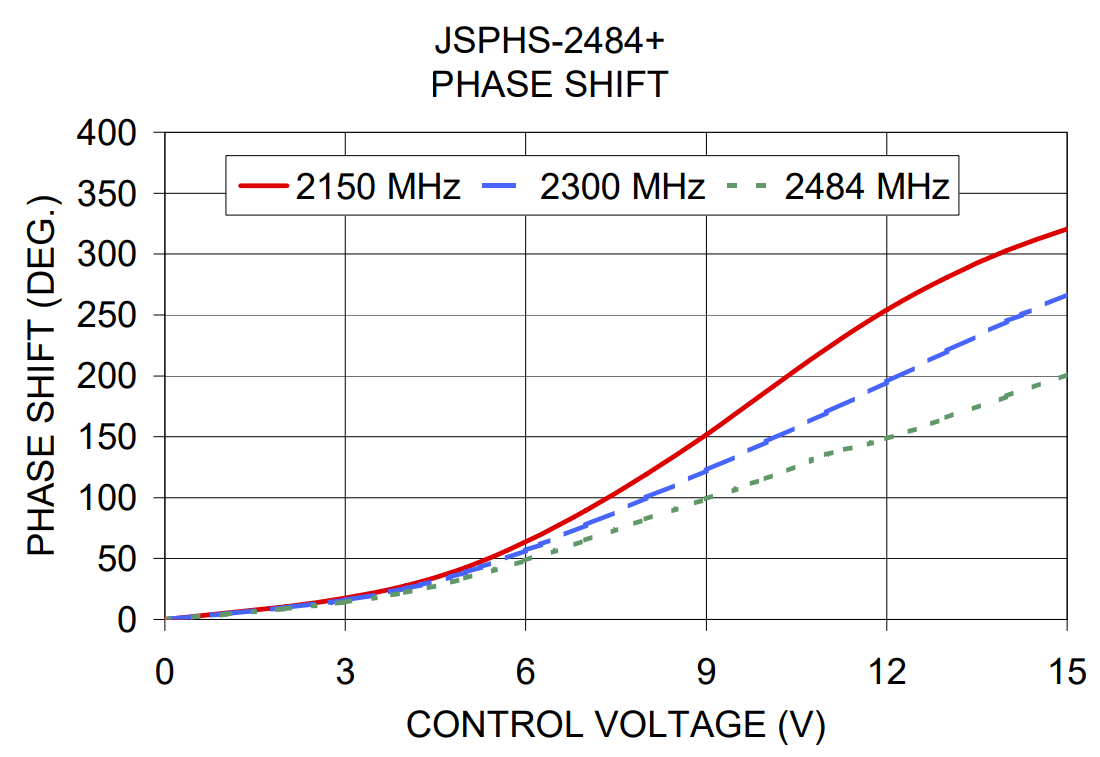
\includegraphics[width=0.6\linewidth]{figs/ch3_JSPHS-2484+PHASE_SHIFT.png}
    \caption{Phase shift (\textdegree) vs Control voltage (V) \cite{PhaseJSPHS-2484+}}
    \label{fig:ch3_JSPHS-2484+PHASE_SHIFT.png}
\end{figure}

\par In this project we are mostly interested in the two frequencies of $2300\:\si{MHz}$ and $2484\:\si{MHz}$ that are shown, up to a maximum of $180^{\circ}$. By analyzing this graphic we can conclude that it would satisfy the goals set for the phase-shifter.

\par Unfortunately, there are other characteristics that can also influence the behavior of the phase-shifter and how it can be integrated into the project. The major two factors  being its \ac{vswr} and \ac{il}. Figures \ref{fig:ch3_JSPHS-2484+VSWR.png} and \ref{fig:ch3_JSPHS-2484+INSERTION_LOSS.png} show two graphs present in the phase-shifter datasheet that detail how these factors change with the \ac{rf} used and the control voltage.

\begin{figure}[H]
    \vspace*{0cm}
    \centering
    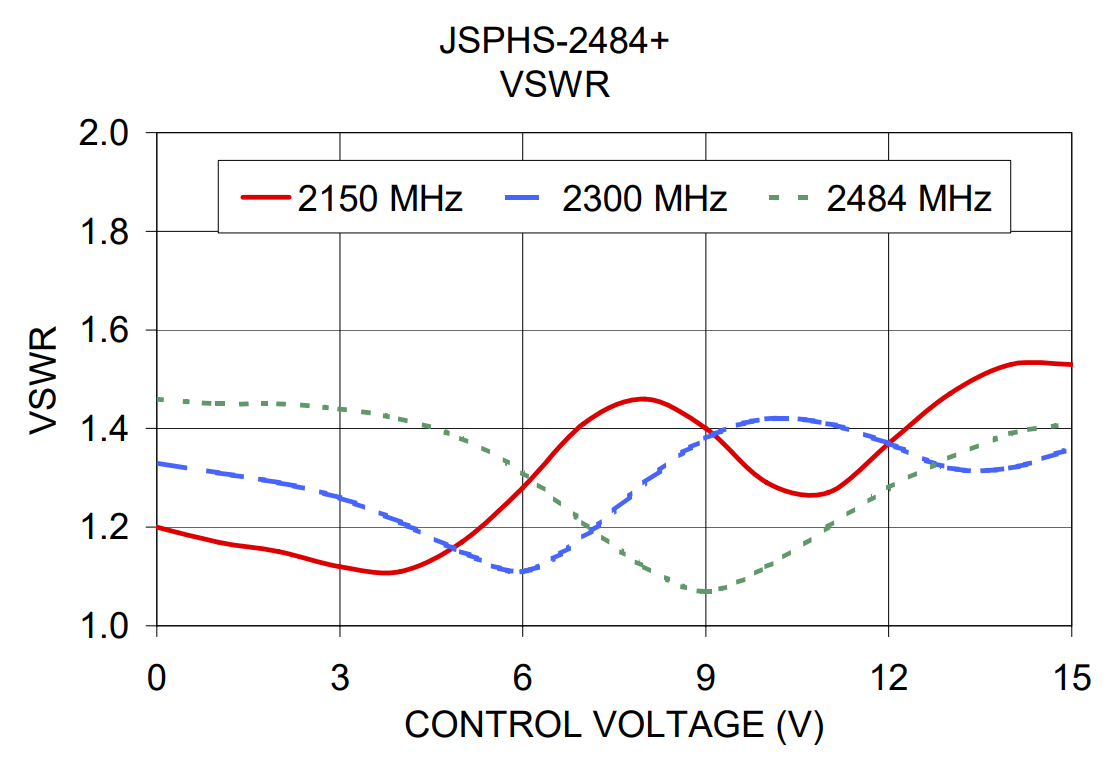
\includegraphics[width=0.6\linewidth]{figs/ch3_JSPHS-2484+VSWR.png}
    \caption{VSWR of JSPHS-2484 \cite{PhaseJSPHS-2484+}}
    \label{fig:ch3_JSPHS-2484+VSWR.png}
\end{figure}

\par We can assume that for the operation conditions that the phase-shifter will be subject in our project, its maximum value for \ac{vswr} would be, rounding up for simplicity, at around $1.5$ for a frequency of $2484 \:\si{MHz}$ when the control voltage is null.

\par Now, the maximum power that the JSPHS-2484 can handle at its \ac{rf} input is $ 20 \:\si{dBm}$.  At the specified \ac{vswr} the power loss in the phase-shift is around $6 \:\si{dBm}$, or $\:\si{0.004W}$. Although not desirable, this amount of power would not necessarily be harmful to the system.

\begin{figure}[H]
    \vspace*{0cm}
    \centering
    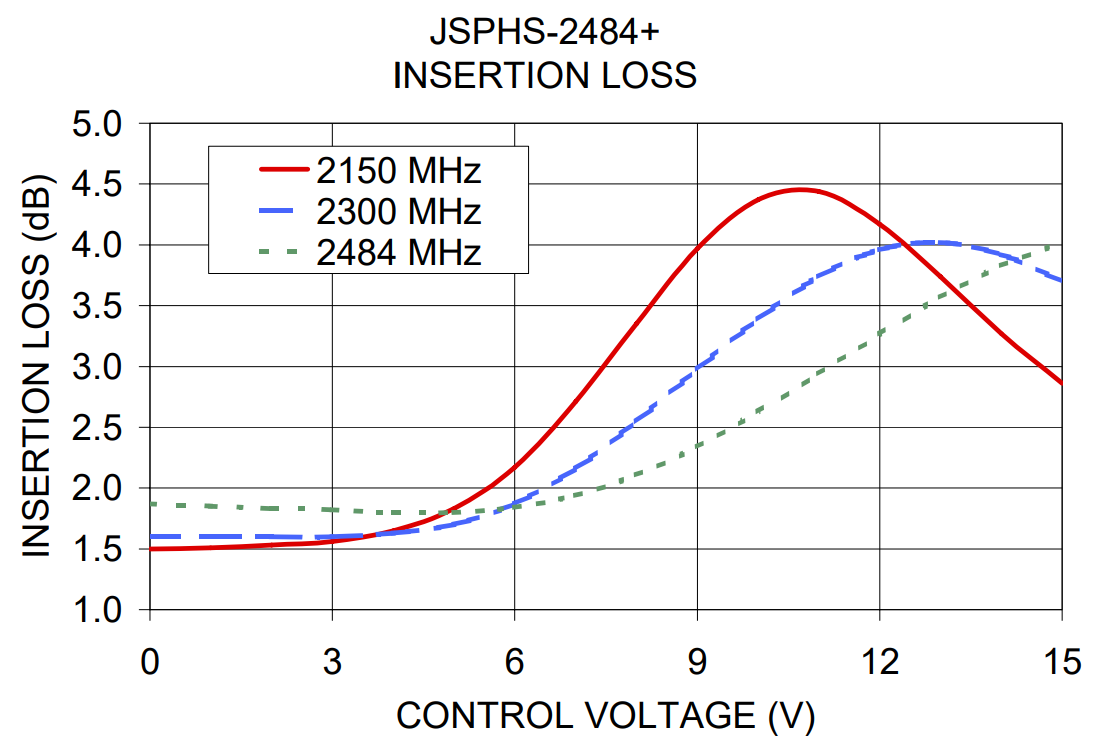
\includegraphics[width=0.6\linewidth]{figs/ch3_JSPHS-2484+INSERTION_LOSS.png}
    \caption{\ac{il} for JSPHS-2484 \cite{PhaseJSPHS-2484+}}
    \label{fig:ch3_JSPHS-2484+INSERTION_LOSS.png}
\end{figure}

\par The most significant of these factors is the \ac{il} as it increases significantly for the desired \ac{rf} reaching almost $3.4 \:\si{dB}$.

\subsection{Quadrature Modulator}
\par For the modulator, the frequency of operation was also a concern. It had to be able to support a carrier signal at a frequency of \ac{rf}.

\par But there was another characteristic that had been specified during the initial phase of the project. The \ac{i} and \ac{q} components that would be be fed to the modulator would operate at a maximum frequency of $20 \:\si{MHz}$. These two requirements alone would help narrow down the list of possible alternatives for this component choice.

\par Another important parameter that was considered was the total power consumed. Some of the devices that were in a convenient price range would have a total power consumption that would be considered somewhat high, at around $900 mW$. Due to the fact that the system would be encapsulated within a compact enclosure, this could be considered a problem. The unnecessary heat added to the heat already expected to be generated by a $10 W$ \ac{pa} could be a problem.

\par In the end, the LTC5589IUF from Analog Devices was chosen as what was thought to be the appropriate quadrature modulator to be used for the project.

\par Unfortunately, during the vetoing of this component, two I made two oversights. The first was to misunderstand the output power of this device. This lead to the belief that the LTC5589IUF would have a gain of $0 \:\si{dB}$, meaning that the signal at the output would have the same power as at the input. In reality, the gain of this device can be interpreted from the following graph taken from the datasheet of the component that is present in Figure \ref{fig:ch3_GainVCTRLquadmod.png}. The gain would actually be closer to $-10 \:\si{dB}$, as the parameter $V_{CTRL}$ was set at $3.3 \:\si{V}$ in the designed prototype.

\begin{figure}[H]
    \vspace*{0cm}
    \centering
    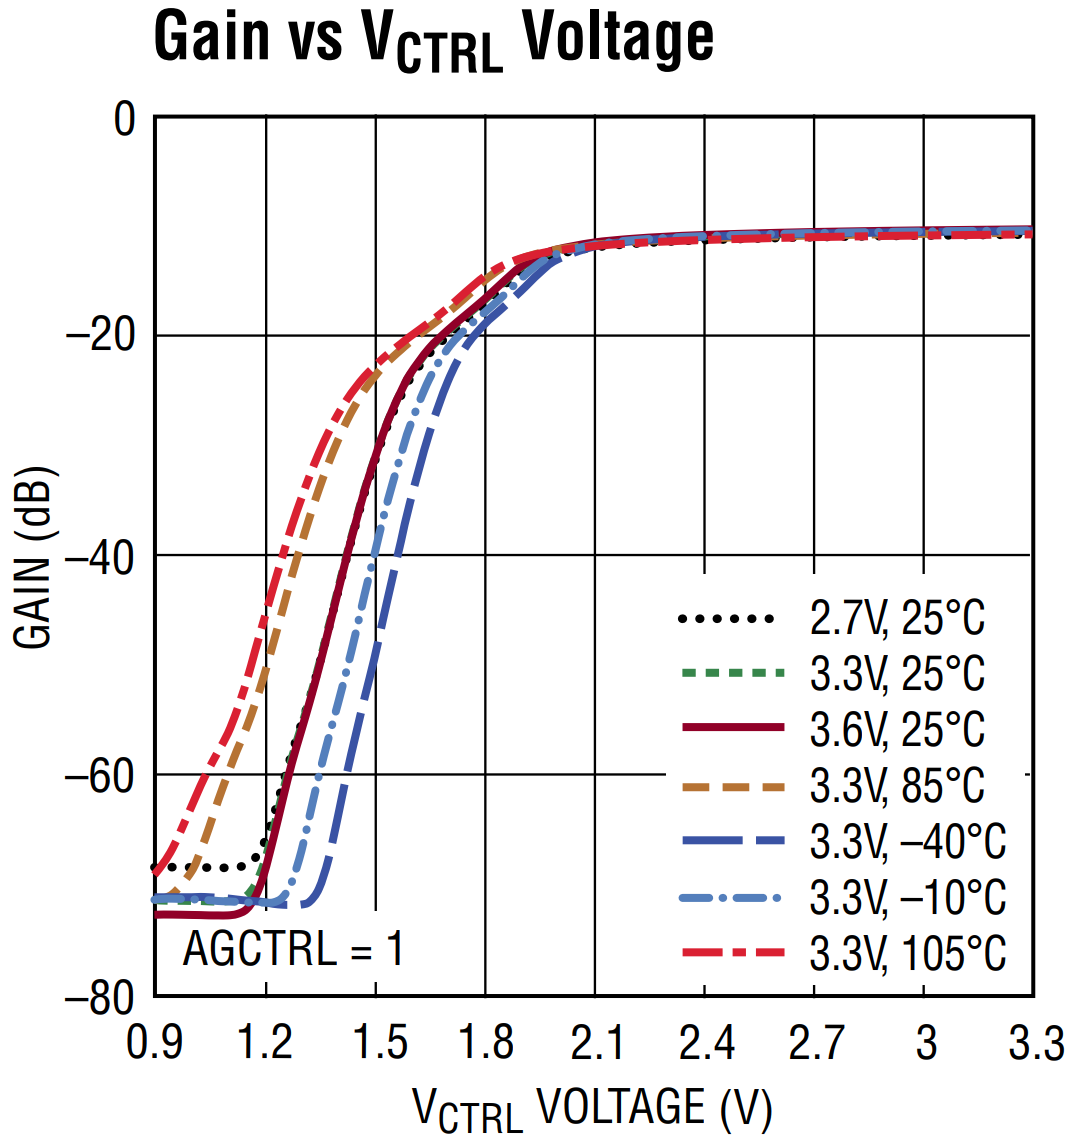
\includegraphics[width=0.6\linewidth]{figs/ch3_GainVCTRLquadmod.png}
    \caption{Relationship of analog gain with $V_{CTRL}$ \cite{LTC5589}}
    \label{fig:ch3_GainVCTRLquadmod.png}
\end{figure}

\par Another characteristic of the LTC5589IUF modulator, and, in fact, of other component used in the project, was its footprint and size. This component is in a QFN package with $4 \:\si{mm}$ sides, with 24 total leads and a thermal pad. Even with the help of Professor Telmo Cunha and the technical expertise of Paulo Gonçalves, it would turn out to be a rather complicated component to properly solder onto the \ac{pcb}. 

\par Another modulator that could have been used would have been the TRF3705IRGET from Texas Instruments. This component can work at the desired frequency, had a gain of approximately $2 \:\si{dB}$ at $2.6 \:\si{GHz}$ and could achieve a maximum output of $6.5 \:\si{dBm}$ at $2.4 \:\si{GHz}$. However, this would also be a QFN package component, which means that the soldering procedure would remain rather difficult. The only major mechanical difference between the TRF3705IRGET and the LTC5589IUF is that the pad underneath the component is thermal rather than connected to ground. This pad is needed because the component will consume more $276.5 \:\si{mA}$ over the LTC5589IUF, totaling $306 \:\si{mA}$.

\subsection{Power Supply} 
\par At this point, there were enough known variables about the project that the choice for a suitable component and subsequent circuitry could be made. The supplied voltage would be $28 \:\si{V}$ and the modulator would work at a supply voltage of $3.3 \:\si{V}$. As such, there was a need to find a component that could be used in a \ac{smps}. This \ac{smps} would be configured as a Buck converter.

\par These two constraints alone were enough to narrow down the number of possible components to be used for the project quite significantly.

\par After some considerations regarding the possibility of a driver amplifier for the \ac{pa}, the switching regulator MC33063ADR from Texas Instruments was chosen. The MC33063ADR could handle up to $1.5 \:\si{A}$ output current with an efficiency of around $83.7\%$. 

\par It could achieve this without the need for many external components. The simplified schematic of this component is presented in the datasheet shown in Figure \ref{fig:ch3_smpsInternal.png}.

\begin{figure}[H]
    \vspace*{0cm}
    \centering
    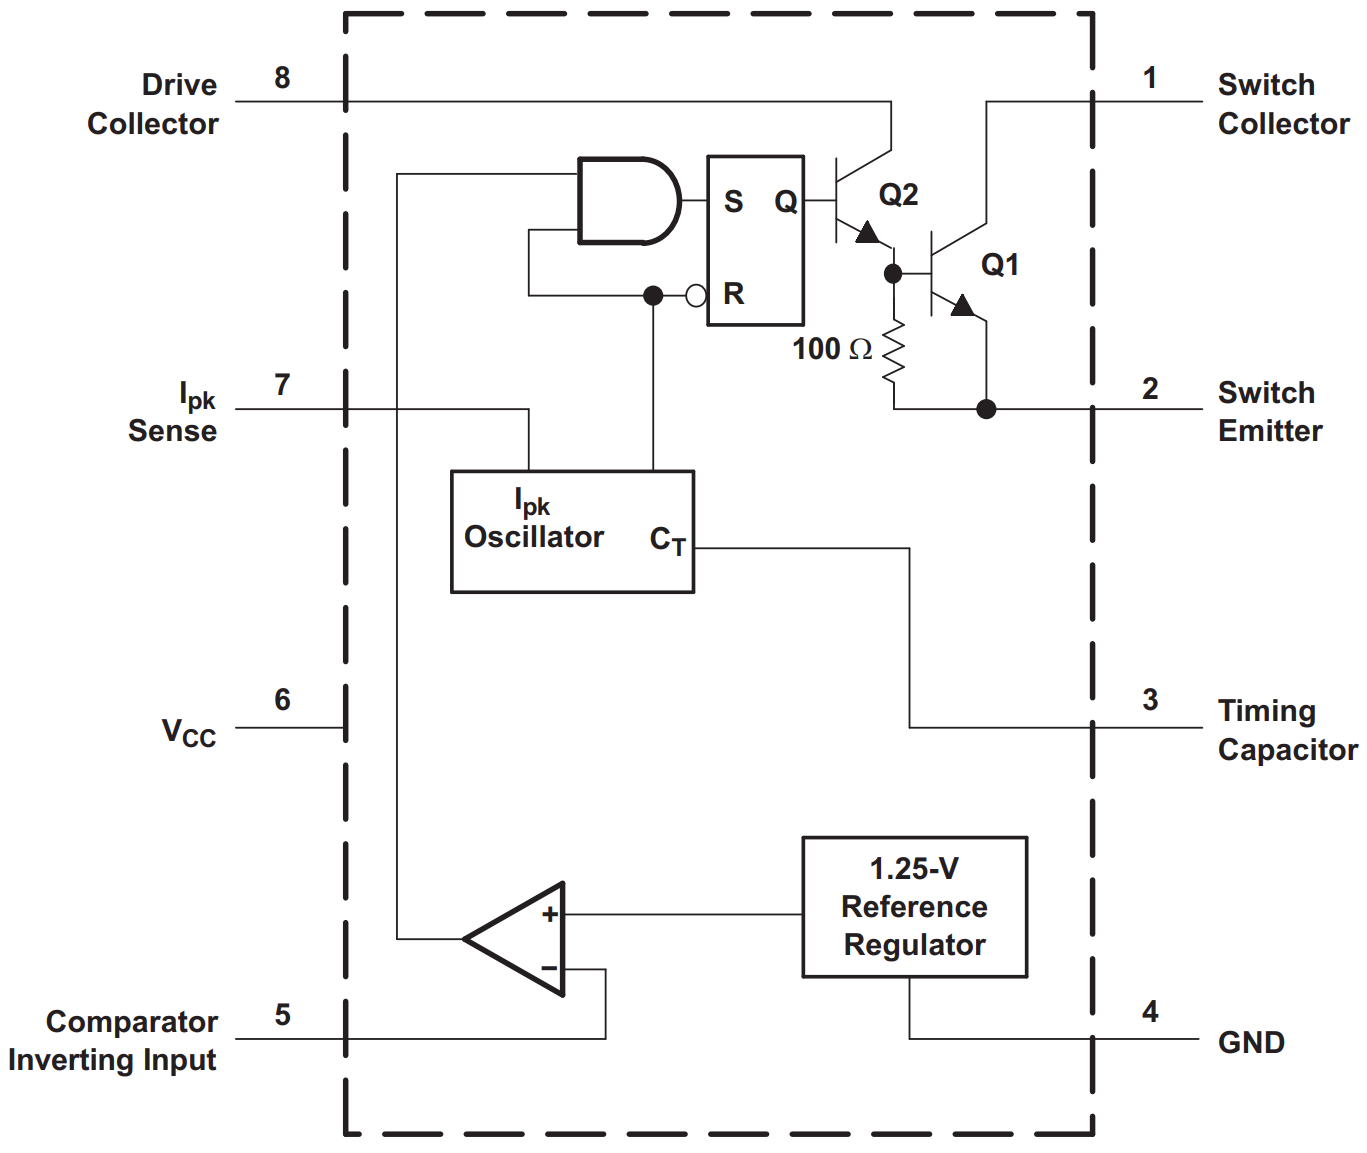
\includegraphics[width=0.6\linewidth]{figs/ch3_smpsInternal.png}
    \caption{Simplified schematic for the MC33063ADR switching regulator \cite{2004MC3x063ARegulators}}
    \label{fig:ch3_smpsInternal.png}
\end{figure}

\par As we can see, the MC33063ADR is a package that already has the internal circuitry needed for many of the requirements of a basic buck converter. There would be no need for external transistors, comparator, oscillator, or voltage references. However, it would require other components depending on the application.

\subsection{Driver Amplifier}
\par For this driver amplifier, some desirable characteristics were considered during selection. The first was the operating frequency range. It had to include the desired \ac{rf} of $2.4 \:\si{GHz}$. Secondly, all the components that had been chosen so far would require a supply voltage of $3.3 \:\si{V}$, so the driver amplifier would be limited to this voltage.

\par As a driver amplifier, this component would be expected to have a high enough gain, since \ac{pa} are often lacking in this parameter.

\par Another factor that influenced the decision process was how easy the amplifier would be to integrate with the rest of the circuit. Meaning, if there was any need for matching any ports, as the initially thought process behind the project would be to try and assemble the whole system with the most ease.

\par After searching through the major online retailers, it was decided on the PGA-102+ monolithic amplifier from Mini-Circuits. 

\par This amplifier can work with the supply voltage of $3.3 \:\si{V}$ and uses a maximum of $83 \:\si{mA}$ It advertises a gain of approximately $13 \:\si{dB}$ at $2.4 \:\si{GHz}$ with a P1dB of $17.5 \:\si{dBm}$ at this frequency. Unfortunately, it was noticed after the circuit was assembled that this low P1dB would limit the output power of the circuit to a maximum of approximately $28 \:\si{dBm}$, which was lower than expected.

\par This amplifier was already matched internally, which meant that its application would be easier. 

\par However, this amplifier would still require some external components for proper \ac{rf} applications. A bias-tee and some block or bypass capacitors would need to be present, according to the manufacturer, as can be seen in the recommended application circuit from the datasheet shown in Figure \ref{fig:ch3_pga102+application.png}. 

\begin{figure}[H]
    \vspace*{0cm}
    \centering
    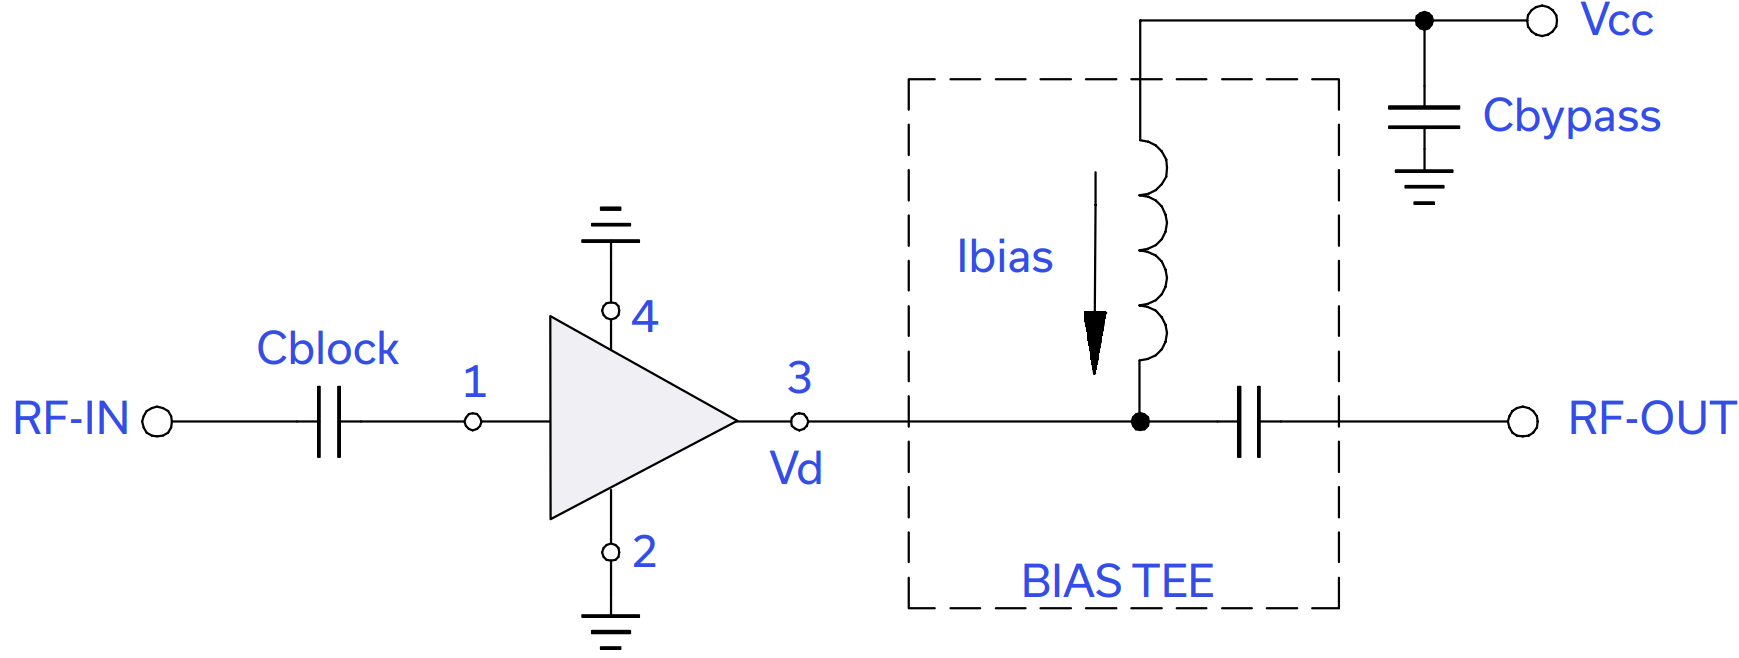
\includegraphics[width=0.7\linewidth]{figs/ch3_pga102+application.png}
    \caption{Recommended application circuit for a PGA-102+ \cite{MonolithicPGA-102+}}
    \label{fig:ch3_pga102+application.png}
\end{figure}

\par This, however, did not pose a concern that could overthrow the choice made for this component.

\subsection{\textbf{\ac{rf} Power Amplifier}}
\par This component is one of the more important ones in the project. It would need to provide most of the power to the signal that goes out to the antenna. Firstly, this amplifier would be required to be able to deliver the expected $40 \:\si{dBm}$ of peak power.

\par With this in mind and with all other constraints related to the operation of the project, in the end the NPA1007 \ac{pa} from MACOM was chosen. This device provides $10.5 \:\si{dB}$ of gain at an input power of $30 \:\si{dBm}$.

\par This amplifier also has its input already matched, which means that it is only required to match the output of the amplifier. The datasheet already details how this can be done. The datasheet also details the procedure for turning on and off the device. 

\par Unfortunatly, the drain efficiency of the amplifier for the desired output power is around $40\%$. This means that a lot of power will be turned into heat. For an operating output power of $40 \:\si{dBm}$ it would be expected to produce around $13 W$ of heat.

\subsection{Enclosure}
\par As mentioned previously, the idea would be for each element of the array to be as close to each other as possible in order for the antennas to be spaced about half a wavelength from each other. For an application at $2.4 \:\si{GHz}$, this means a distance of around $6.3 \:\si{cm}$ or $2.46 \:\si{in}$, rounded up to the millimeter. This measure would be critical, as it would determine the maximum width and height of the enclosure. There was no restriction for the total depth of the box, as long as it was reasonable. Ideally, this enclosure would be metal so that the circuits inside could be shielded. But after an unsuccessful search, this criteria was abandoned, and the search also started including other materials.

\par There was also the fact that this enclosure would have to undergo some modifications if we wanted to have some sort of front panel connections on one side of the box, and leave a whole to properly bias the power amplifier.

\par In the end, the Bud Industries CU-793-MB model was chosen as a suitable enclosure. This box has a width of $2.23 \:\si{in}$, or $5.66 \:\si{cm}$, on the top that then tapers to $2.125 \:\si{in}$, or $5.4 \:\si{cm}$, on the bottom, as can be seen in Figure \ref{fig:ch3_CU-793-MB.png}. This box has a depth of around $4 \:\si{in}$, or $10.16 \:\si{cm}$.

\begin{figure}[H]
    \vspace*{0cm}
    \centering
    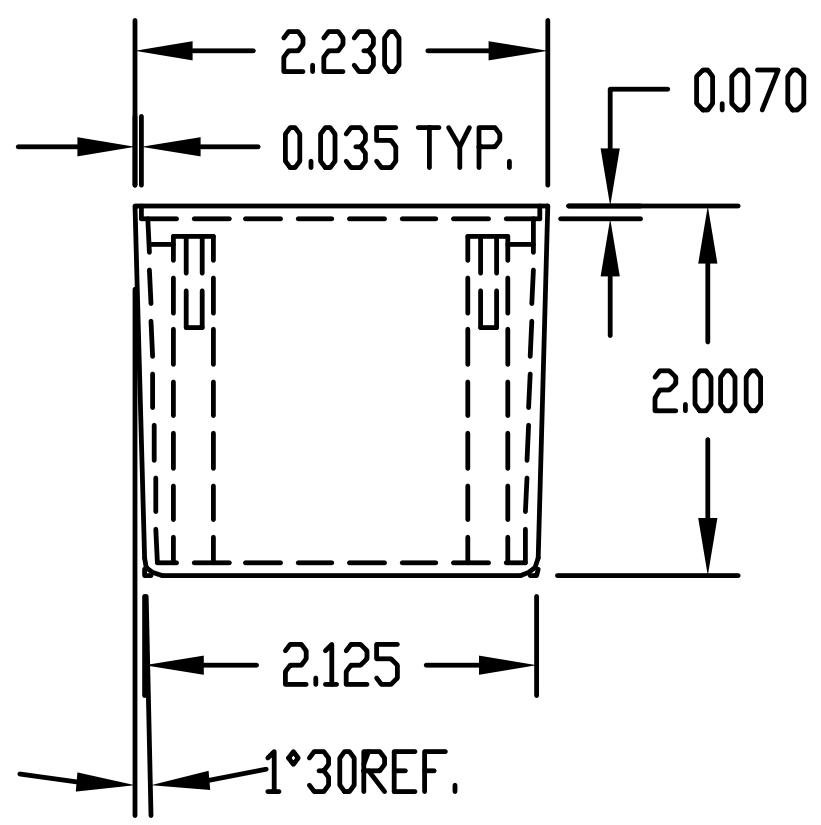
\includegraphics[width=0.4\linewidth]{figs/ch3_CU-793-MB.png}
    \caption{Dimensions of the external face of the enclosure \cite{UtiliboxCUR-793}}
    \label{fig:ch3_CU-793-MB.png}
\end{figure}

\par This choice will also set the limits for the future \ac{pcb} to be used for the project.

\subsection{Connectors and \ac{pcb} substrate}
\par For the substrate of the \ac{pcb}, we will use the same that is recommended by MACOM to the NPA1007 \acl{pa}. It is the Rogers RO4350B with a thickness of $0.508 \:\si{mm}$.

\par One of the requirements of this project would be to be able to have all the signals delivered to the array element via a front panel. To do this, we would have to bridge the gap from the \ac{pcb} to the outside. 

\par For the carrier wave signal, this could be done by simply adding an SMA connector to the edge of the \ac{pcb} and drilling a hole in the box, having it protrude in order to be accessible from the outside. The connector used is CON-SMA-EDGE from FR Solutions.

\par To deliver the \ac{iq} signals, as it would be impossible to mount many more connectors on the \ac{pcb} edge, we needed to have some way of having a cable come from the \ac{pcb} to another place on the box. We used on cable CSI-SGFB-100-UFFR for both the \ac{i} and \ac{q} components. This would then connect to two CONUFL001-SMD-T on the board. All of these are from TE Connectivity.

\par For all other signals, $28 \:\si{V}$, $-5 \:\si{V}$, GND and the signal to control the phase-shifter, the connector 43045-0658 from Molex was chosen. It would also be placed on the edge of the \ac{pcb}, and would have the cable 214756-1061 from Molex connected to it. The wires from the cable could then be soldered to the wires carrying those signals. It is worth mentioning that there are 4 signals and the connector has 6 available slots. It was decided that two extra connections could be used in case there was need to feed another connection into the box.

\section{Implementation}
\par In this section, there will be an explanation of how each component was used and integrated in the circuit designed for the \ac{psa}. Many of these are based on application notes from the datasheets of the components being used.

\subsection{LTC5589}
\par For the quadrature modulator, the implementation follows very closely what the datasheet explains in its application information section that can be seen in Figure \ref{fig:ch3_LTC5589_application.png}. There are, however, some differences. The circuit shown in this figure makes use of the \ac{spi} protocol pins. We will not be making use of this protocol and, as such, the circuit will differ here.

\begin{figure}[H]
    \vspace*{0cm}
    \centering
    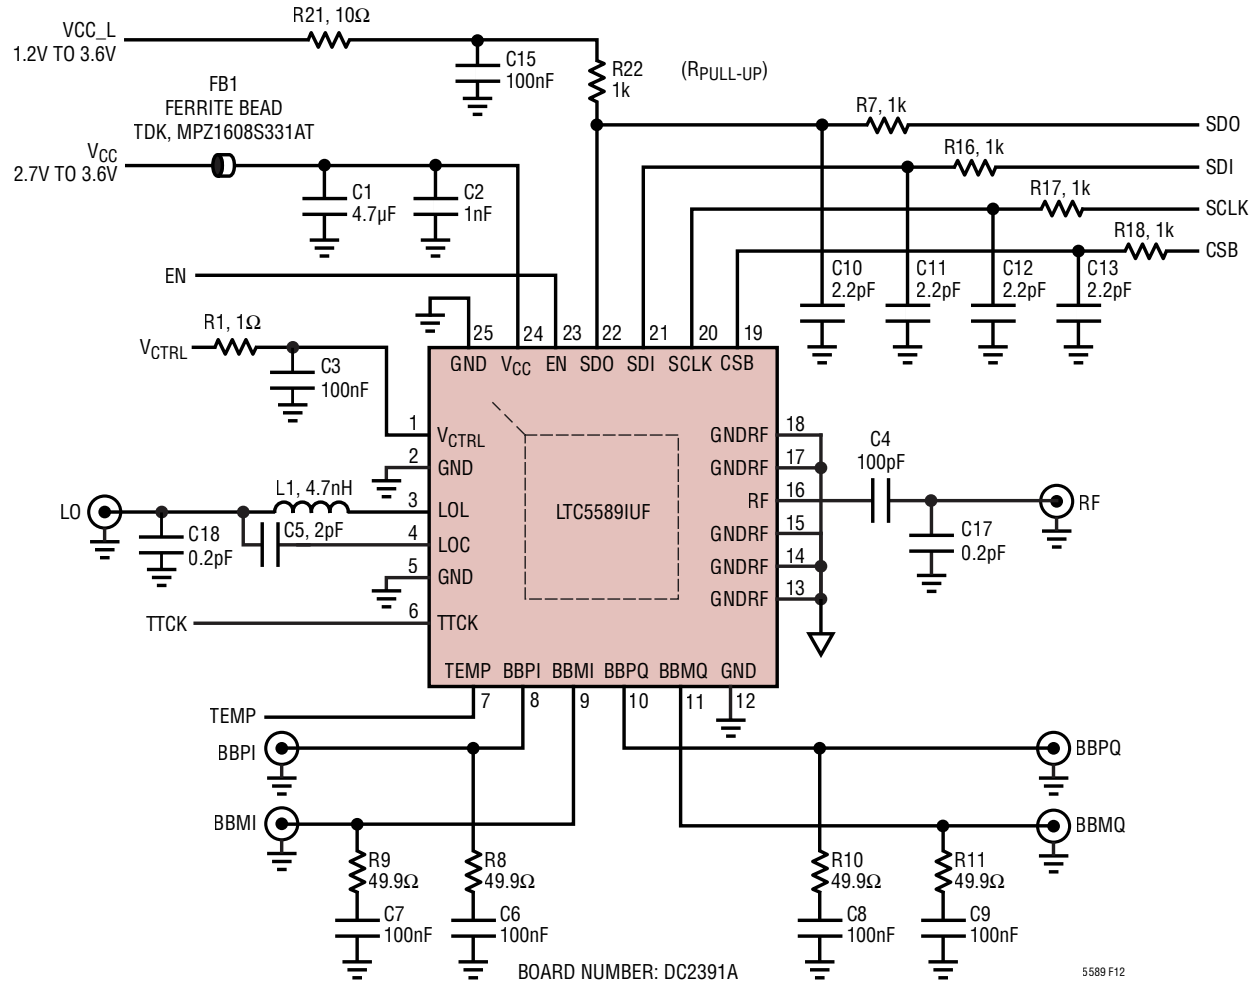
\includegraphics[width=0.7\linewidth]{figs/ch3_LTC5589_application.png}
    \caption{Recommended application circuit for the LTC5589 Modulator \cite{LTC5589}}
    \label{fig:ch3_LTC5589_application.png}
\end{figure}

\par Because of this, for our circuit, pins 19 through 22 will be grounded, as the datasheet warns that, for applications where \ac{spi} is not used, the pins must not be left floating.

\par There is also the fact that the modulator will not be digitally controlled. We are interested only in setting it up and not having to worry about it anymore. As such, we will be changing some other pin configurations in order to have the LTC5589 working as the project requires.

\par The pin responsible for the Variable Gain Control Input, $V_{CTRL}$ (pin 1), is going to be connected to $3.3\:\si{V}$, in order to set the modulator to operate with the maximum gain factor that it can.

\par As we have no interest in measuring the temperature of the modulator, pins 6 and 7, TTCK and TEMP respectively, will both be connected to ground. The datasheet explicitly warns against leaving pin 6 floating.

\par Pin 23 would allow us to control whether or not the component is completely on. For the purpose of this project, the modulator will always work properly and, as such, will be directly connected to $3.3\:\si{V}$. Once again, it is advised that the pin should not be left floating.

\subsubsection{Baseband signals \ac{i} and \ac{q}}
\par The LTC5589 quadrature modulator has some particular requirements when it comes to supplying it with appropriate \ac{i} and \ac{q} components. It mentions that the signals must be supplied to the device as differential inputs to the BBPI, BBMI pins for the \ac{i} signal and BBPQ, BBMQ for the \ac{q} signal. These signals must have a common mode level of $1.4\:\si{V}$ up to $2.0\:\si{V}$, as specified by the datasheet.

\par In order to interface the device with the signals for the modulator, a circuit block that would convert these single ended signals into differential signals had to be designed. 

\par For this circuit, two OpAmps were used, in a configuration equal to the one seen in Figure \ref{fig:ch3_LTC5589interfaceCirc.png}, which is explained in a Texas Instruments's application note. The OpAmps chosen for this circuit were OPA2607IDR from Texas Instruments.

\begin{figure}[H]
    \vspace*{0cm}
    \centering
    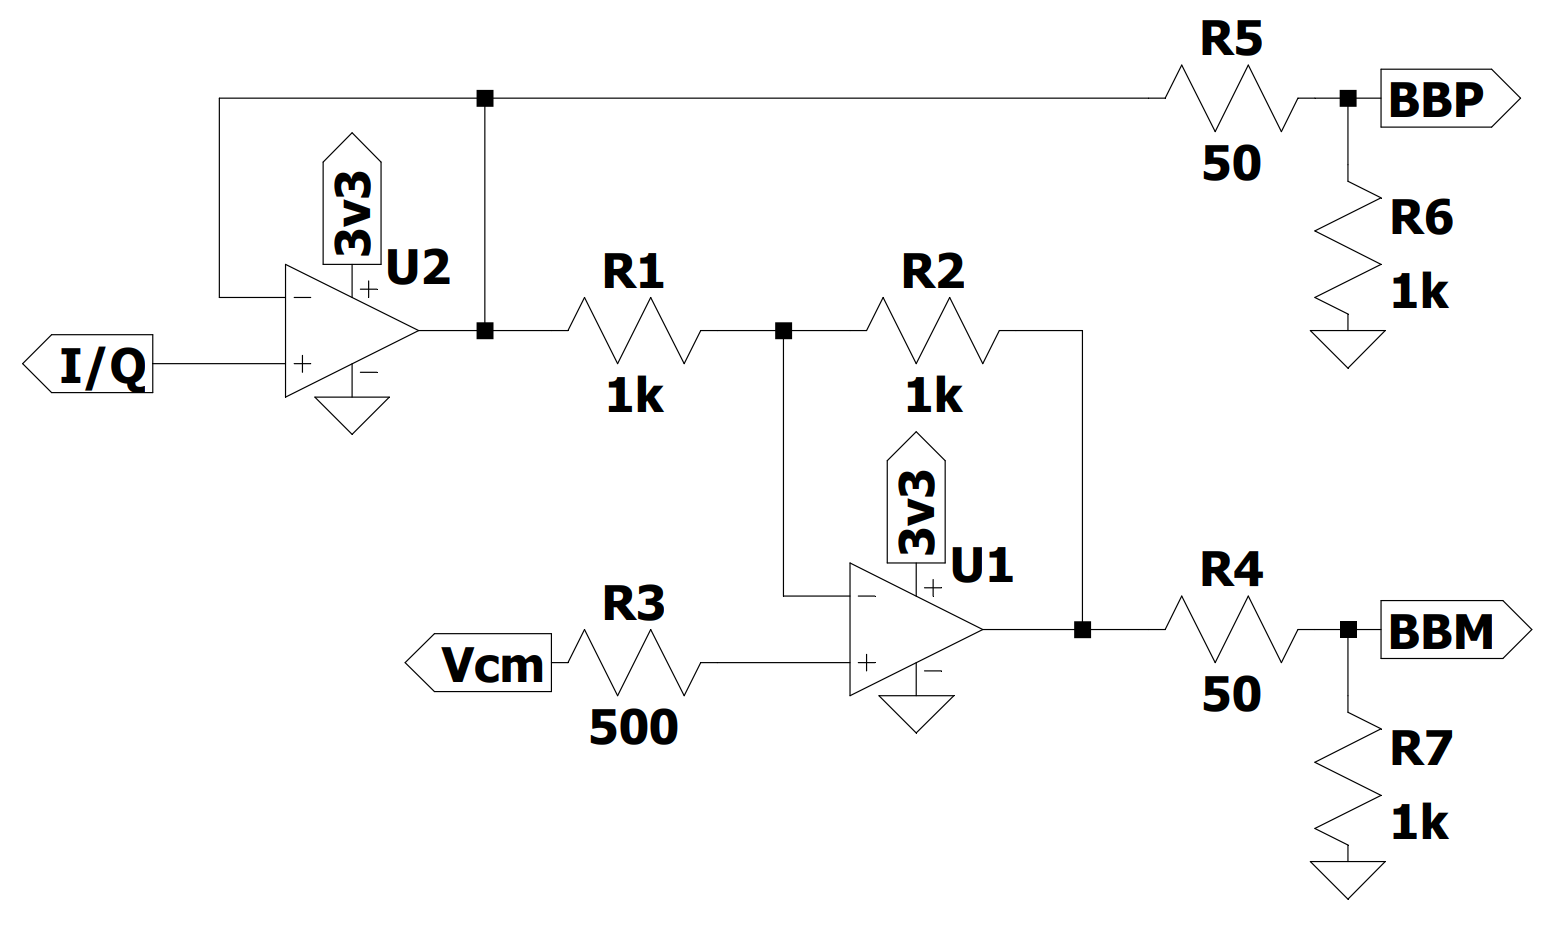
\includegraphics[width=0.7\linewidth]{figs/ch3_LTC5589interfaceCirc.png}
    \caption{Circuit block to interface \ac{iq} signals: single ended to differential}
    \label{fig:ch3_LTC5589interfaceCirc.png}
\end{figure}

\par For this circuit block, a simulation is performed using LTSpice, Analog Devices SPICE simulator software, that results in the output seen in Figure \ref{fig:ch3_LTC5589interfacePlot}.

\begin{figure}[H]
    \vspace*{0cm}
    \centering
    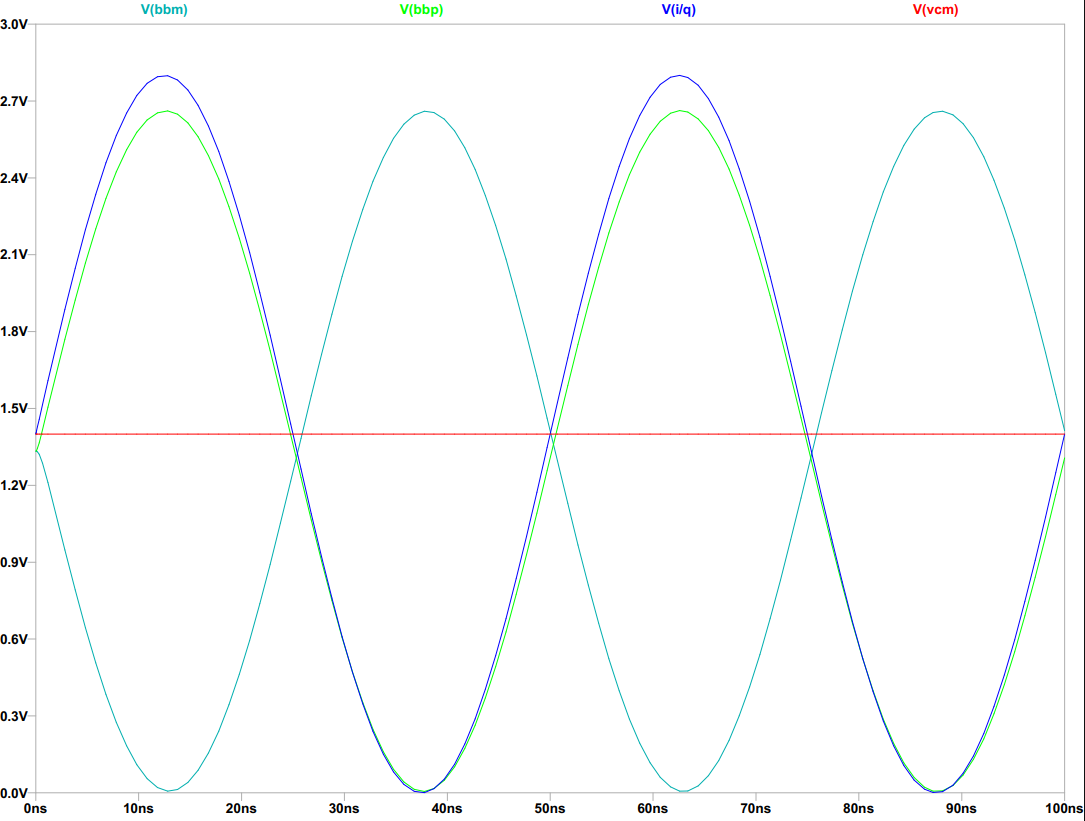
\includegraphics[width=0.7\linewidth]{figs/ch3_LTC5589interfacePlot.png}
    \caption{Simulation results of the single ended to differential converter}
    \label{fig:ch3_LTC5589interfacePlot}
\end{figure}

\par There was always a focus on procuring resistors, inductors, and capacitors capable suitable for operating at the frequencies to which they would be subject. This way we would not have to worry about undesirable behaviors that could be caused by parasitic characteristics of each component.

\subsection{Buck Converter}
\par In order to properly design this section of the circuit, the datasheet of the MC33063ADR section referring to this type of converter was closely followed.

\par We needed to develop a $28\:\si{V}$ to $3.3\:\si{V}$ buck converter. According to the datasheet we first had to define some design parameters for the circuit. 

\begin{itemize}
    \item $V_{SAT} = 0.45\:\si{V}$ for the saturation of the switch;
    \item $V_{F} = 0.45\:\si{V}$ for the forward voltage drop of the retifier;
    \item $I_{O} = 0.5\:\si{A}$ as maximum output current;
    \item $f_{MIN} = 11\:\si{KHz}$ for the minimum frequency at which the circuit would operate;
    \item $V_{R} = 0.05\:\si{V}$ for the maximum peak-to-peak ripple voltage for the output
\end{itemize}

\par Afterwards, we could calculate several values for several components that would allow the Buck converter to operate as we wanted. These values are registered in the following list of external components shown in Figure \ref{fig:ch3_BuckConf.png}.

\begin{itemize}
    \item $C_{T} = 487\:\si{pF}$
    \item $R_{SC} = 0.15\:\si{\Omega}$
    \item $L_{MIN} = 148 \:\si{\mu H}$
    \item $C_{O} = 455 \:\si{\mu F}$
\end{itemize}

\par As these values are not necessarily easy to obtain, as they are not in any common series of components, some compromises had to be made, without detracting from the overall performance of the Buck converter. As such, the components that were used for the project were

\begin{itemize}
    \item $C_{T} = 470\:\si{pF}$
    \item $R_{SC} = 0.33\:\si{\Omega}$
    \item $L_{MIN} = 220\:\si{\mu H}$
    \item $C_{O} = 470\:\si{\mu F}$
\end{itemize}

\par The datasheet also mentions the possibility of adding a filter at the output of the Buck converter. For the project that was being designed, it made sense to use one, as we did not want any undesirable fluctuations of the output voltage. A LC filter was added, with an inductor of $L = 1\:\si{\mu H}$ and a capacitor of $C = 100\:\si{\mu F}$.

\par Two resistors are used to set the desired output voltage, $V_{O}$. To calculate them we can use Equation \ref{ch3_buckResistors}.

\begin{equation}
    \label{ch3_buckResistors}
    V_{O} = 1.25\cdot\left(1+\frac{R2}{R1}\right)
\end{equation}

\par In order to find what was the better pair of values for these resistors, we can try an iterative process until we find two of these values that belong to a series of resistance or are very close to these values. In the end we obtained these values such that $R2 = 1.8\:\si{K\Omega}$ and $R1 = 1.1\:\si{K\Omega}$.

\par The overall design for this block of the project can be seen in Figure \ref{fig:ch3_BuckConf.png}.

\begin{figure}[H]
    \vspace*{0cm}
    \centering
    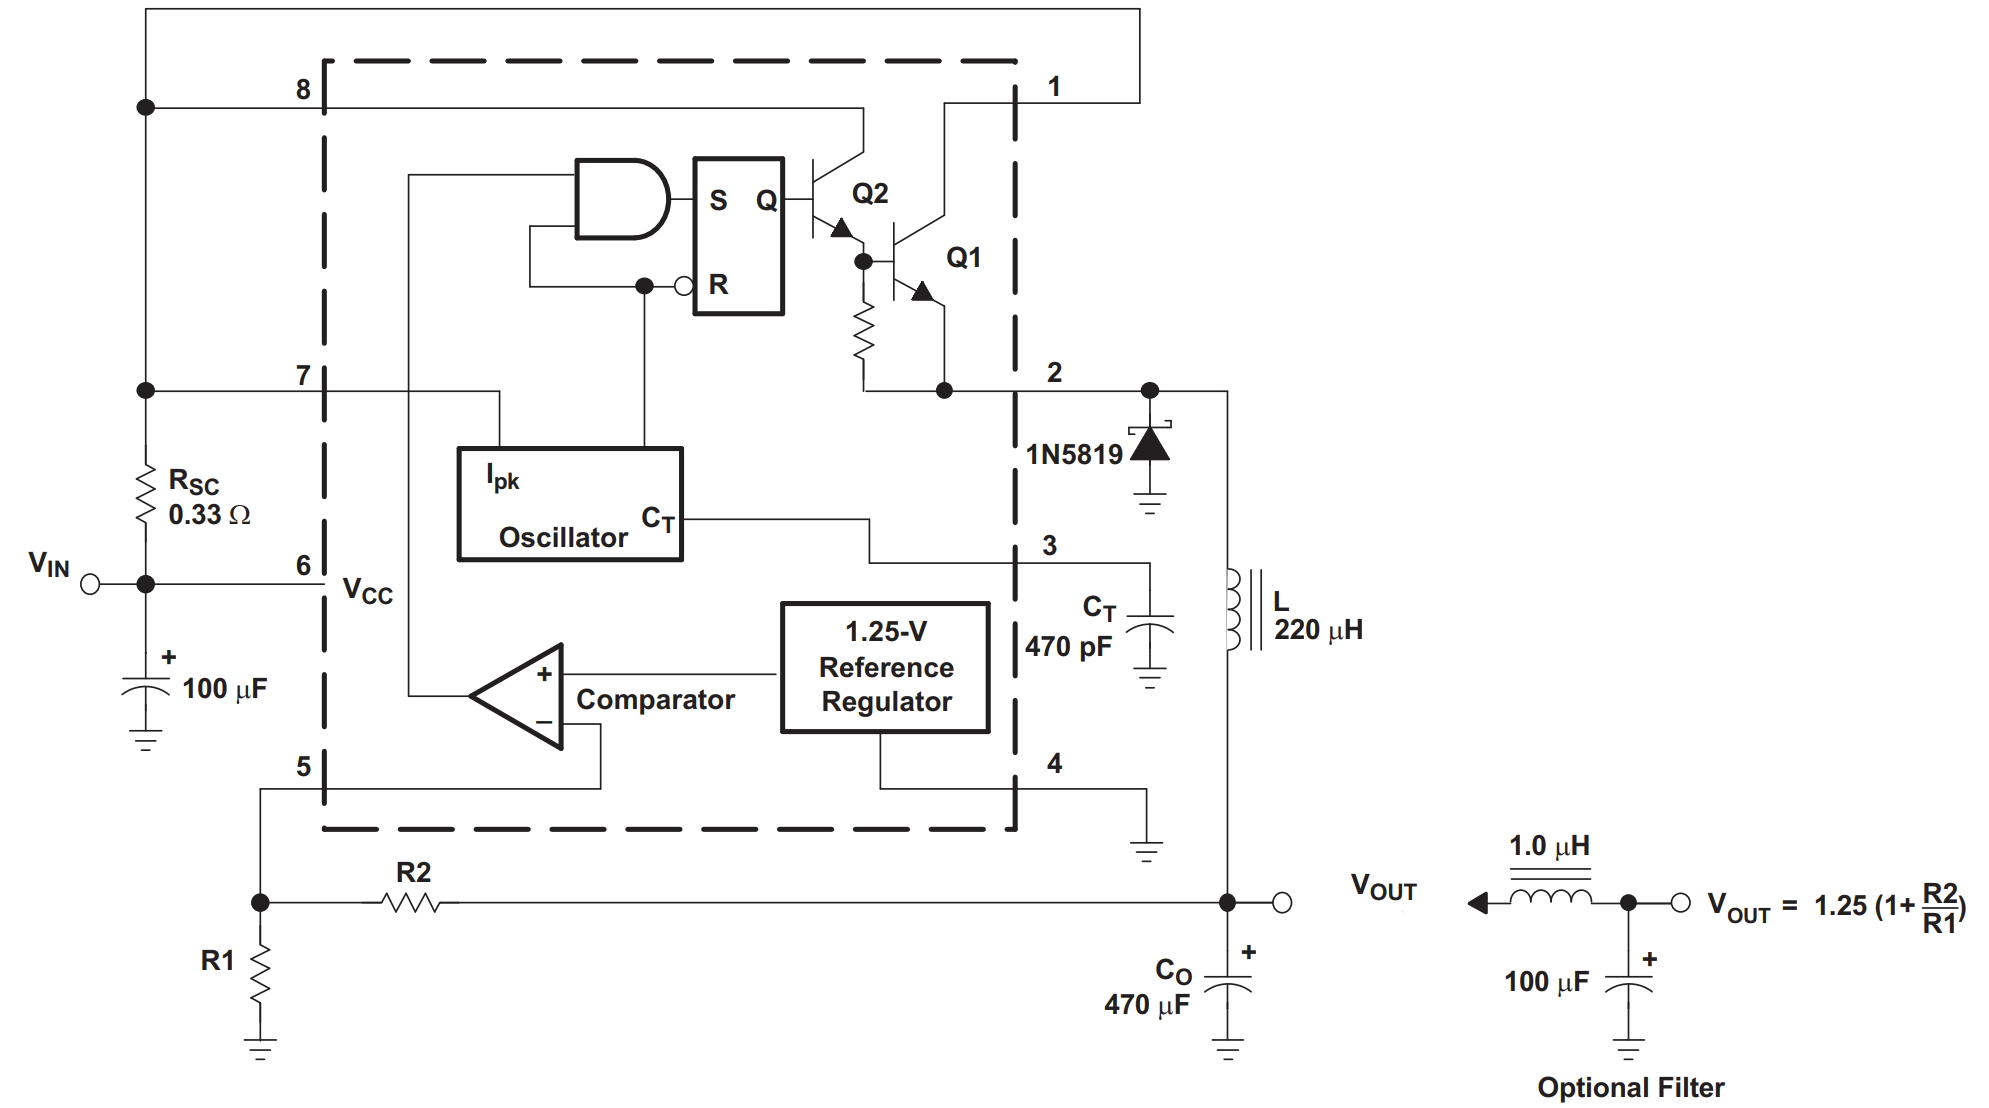
\includegraphics[width=0.9\linewidth]{figs/ch3_BuckConf.png}
    \caption{Buck converter design \cite{2004MC3x063ARegulators}}
    \label{fig:ch3_BuckConf.png}
\end{figure}

\subsection{Driver Amplifier}
\par In order to have the PGA-102r+ in working condition, as mentioned earlier, it needed to have a bias-tee associated with it. There were also two decoupling capacitors used for this component. The bias-tee was designed and simulated within with Keysight's PathWave Advanced Design System.

\par Using the s-parameter files made available by Mini-Circuits for the driver amplifier, we arrived at the following circuit, which is shown in Figure \ref{fig:ch3_PGAbiastee.png}.

\begin{figure}[H]
    \vspace*{0cm}
    \centering
    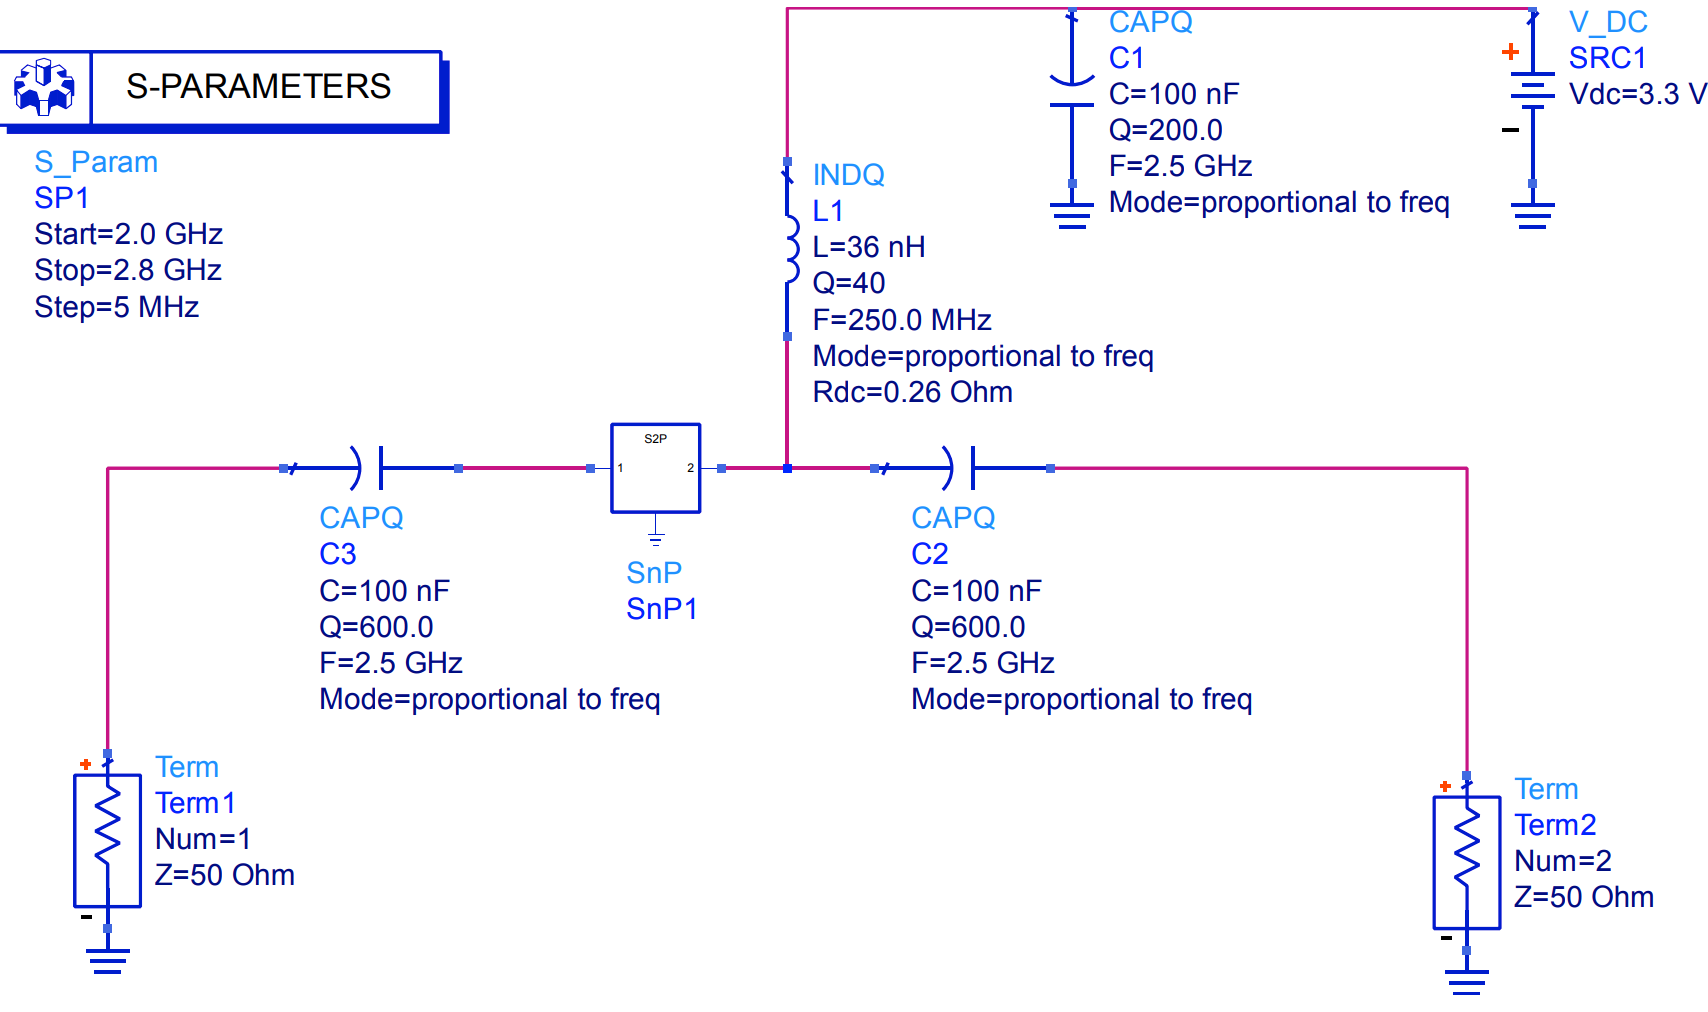
\includegraphics[width=0.9\linewidth]{figs/ch3_PGAbiastee.png}
    \caption{Circuit for the PGA-102+ bias-tee}
    \label{fig:ch3_PGAbiastee.png}
\end{figure}

\par The results obtained after the simulation can be seen in Figure \ref{fig:ch3_PGASim.png}. Here we can see the expected Gain, Input and Output Return Loss. These results are very similar to the expected results from the component datasheet that are shown in Figures \ref{fig:ch3_PGAGainTheo.png} and \ref{fig:ch3_PGAioRLtheo.png}. We are only interested in the results for a frequency of $2.4 \:\si{GHz}$, with a supply of $3.3 \:\si{V}$ and at room temperature.

\begin{figure}[H]
    \vspace*{0cm}
    \centering
    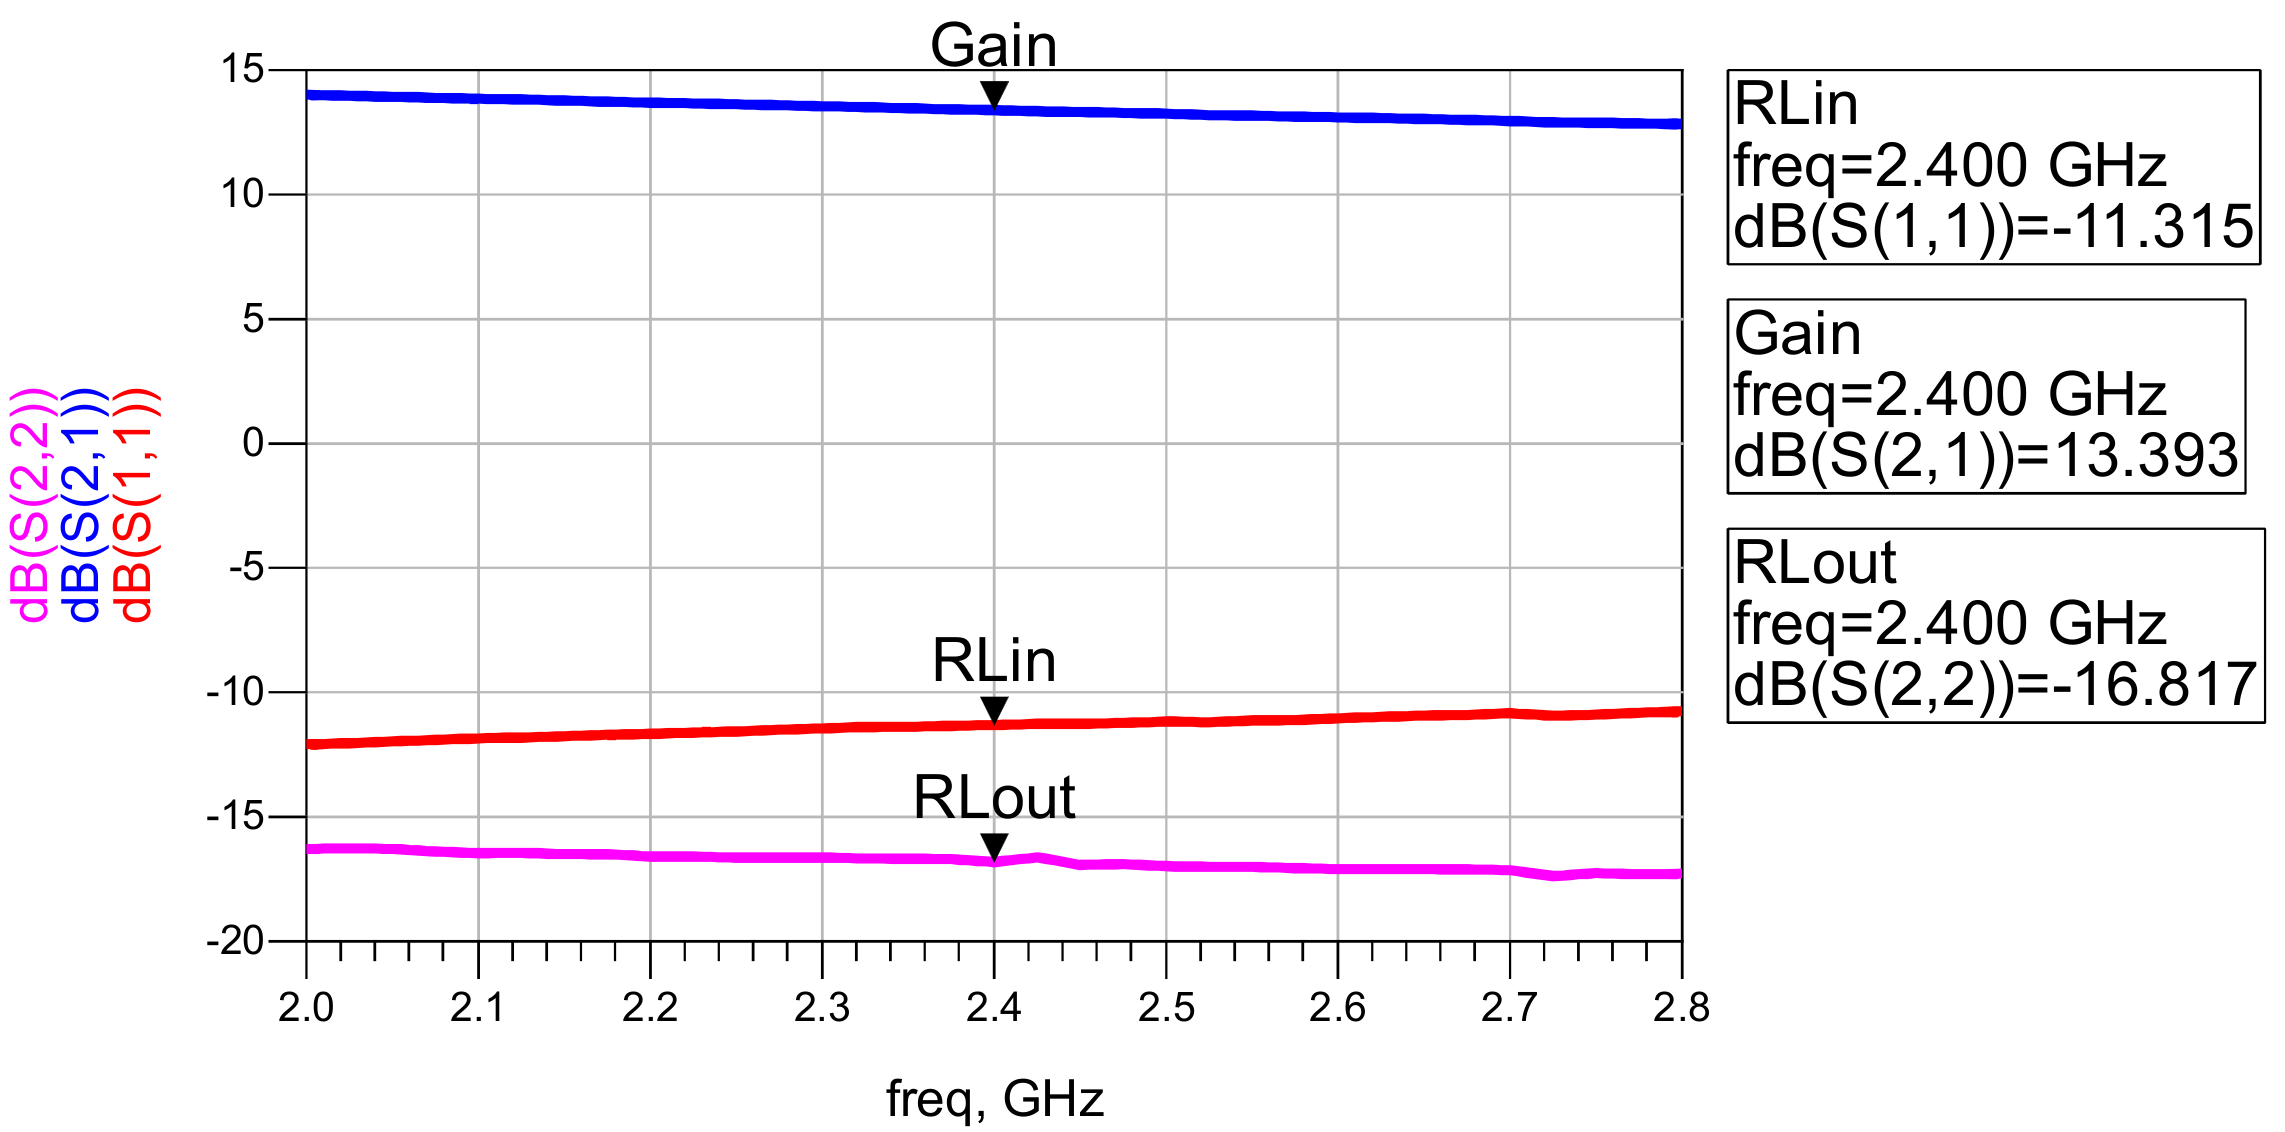
\includegraphics[width=0.9\linewidth]{figs/ch3_PGASim.png}
    \caption{Simulated results of the bias-tee developed}
    \label{fig:ch3_PGASim.png}
\end{figure}

\begin{figure}[H]
    \vspace*{0cm}
    \centering
    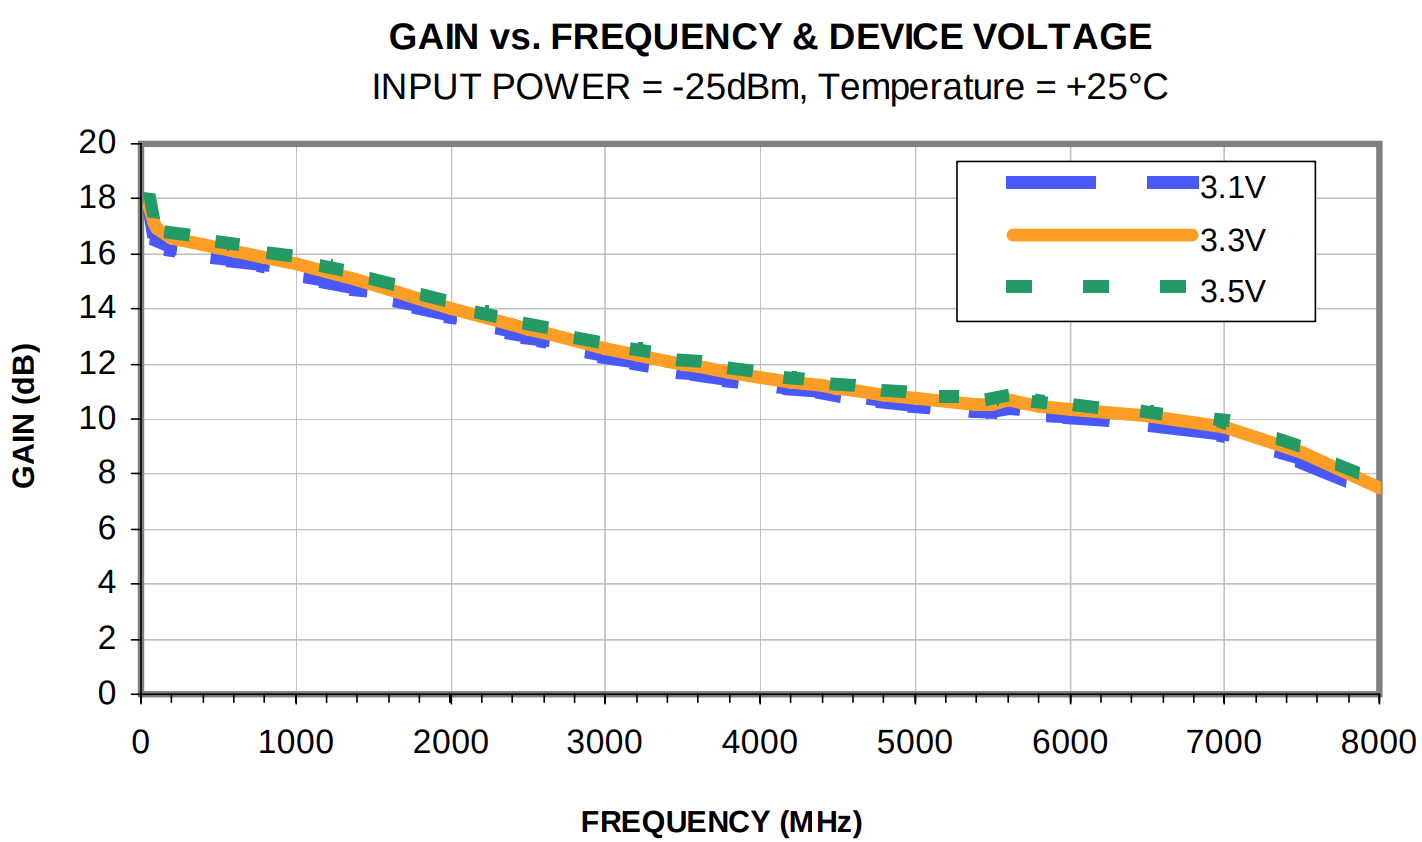
\includegraphics[width=0.9\linewidth]{figs/ch3_PGAGainTheo.png}
    \caption{Expected gain from the datasheet of PGA-102+ \cite{MonolithicPGA-102+}}
    \label{fig:ch3_PGAGainTheo.png}
\end{figure}

\begin{figure}[H]
    \vspace*{0cm}
    \centering
    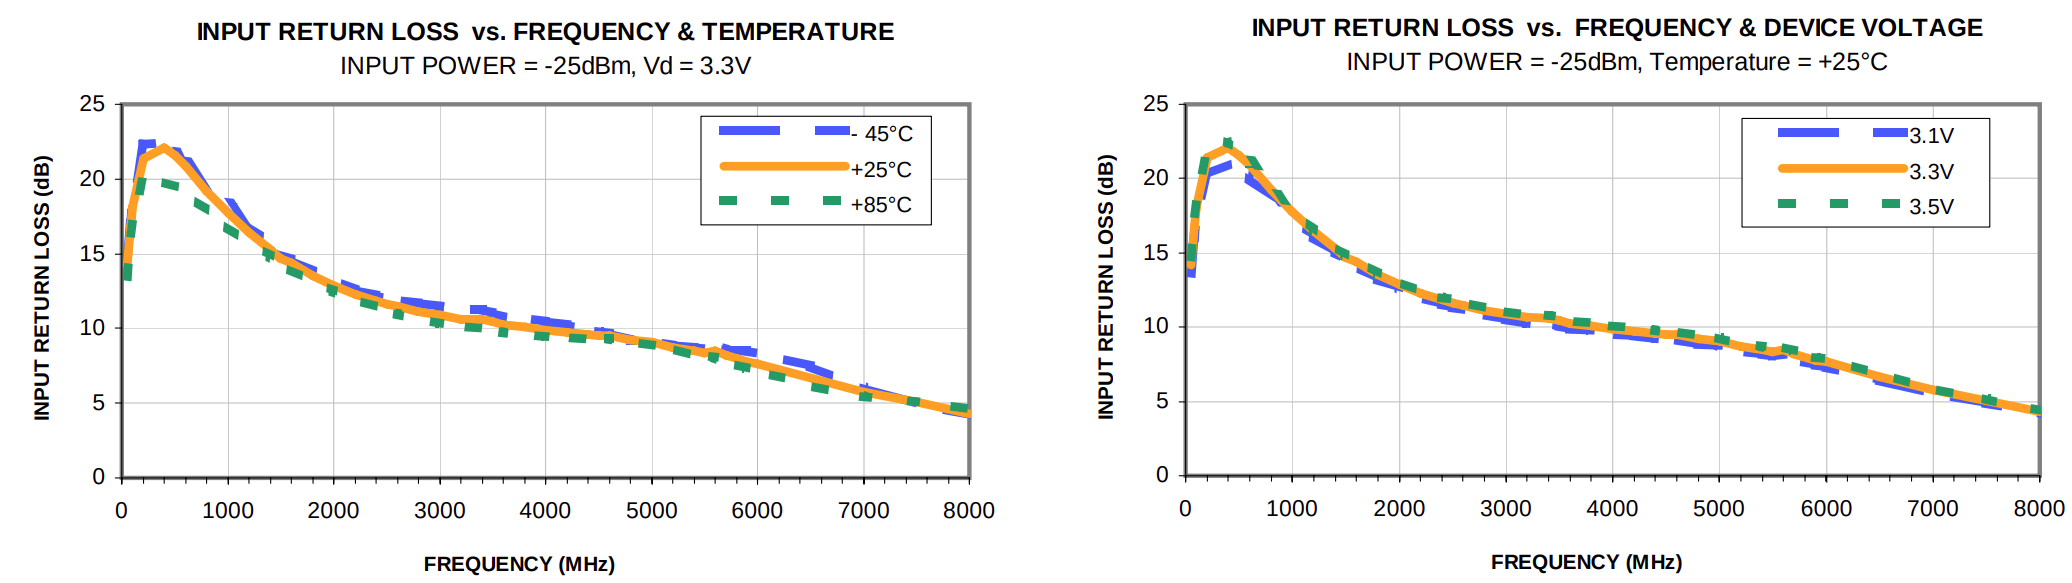
\includegraphics[width=0.9\linewidth]{figs/ch3_PGAioRLtheo.png}
    \caption{Input and Output Return Loss of the PGA-102+ driver amplifier \cite{MonolithicPGA-102+}}
    \label{fig:ch3_PGAioRLtheo.png}
\end{figure}

\par The results obtained were satisfactory and made us comfortable enough with them, so this design choice ended up being used for the project.

\subsection{\acl{pa}}
\par For the circuit assembly of the \ac{pa}, we tried to follow the the evaluation board layout on Figure \ref{fig:ch3_NPA1007eval.png} that is present on the datasheet of the NPA1007, as it was compliant with the majority of the specifications. The only specifications that this design did not respect was the ability to control the gate voltage with a potentiometer or having a circulator.

\begin{figure}[H]
    \vspace*{0cm}
    \centering
    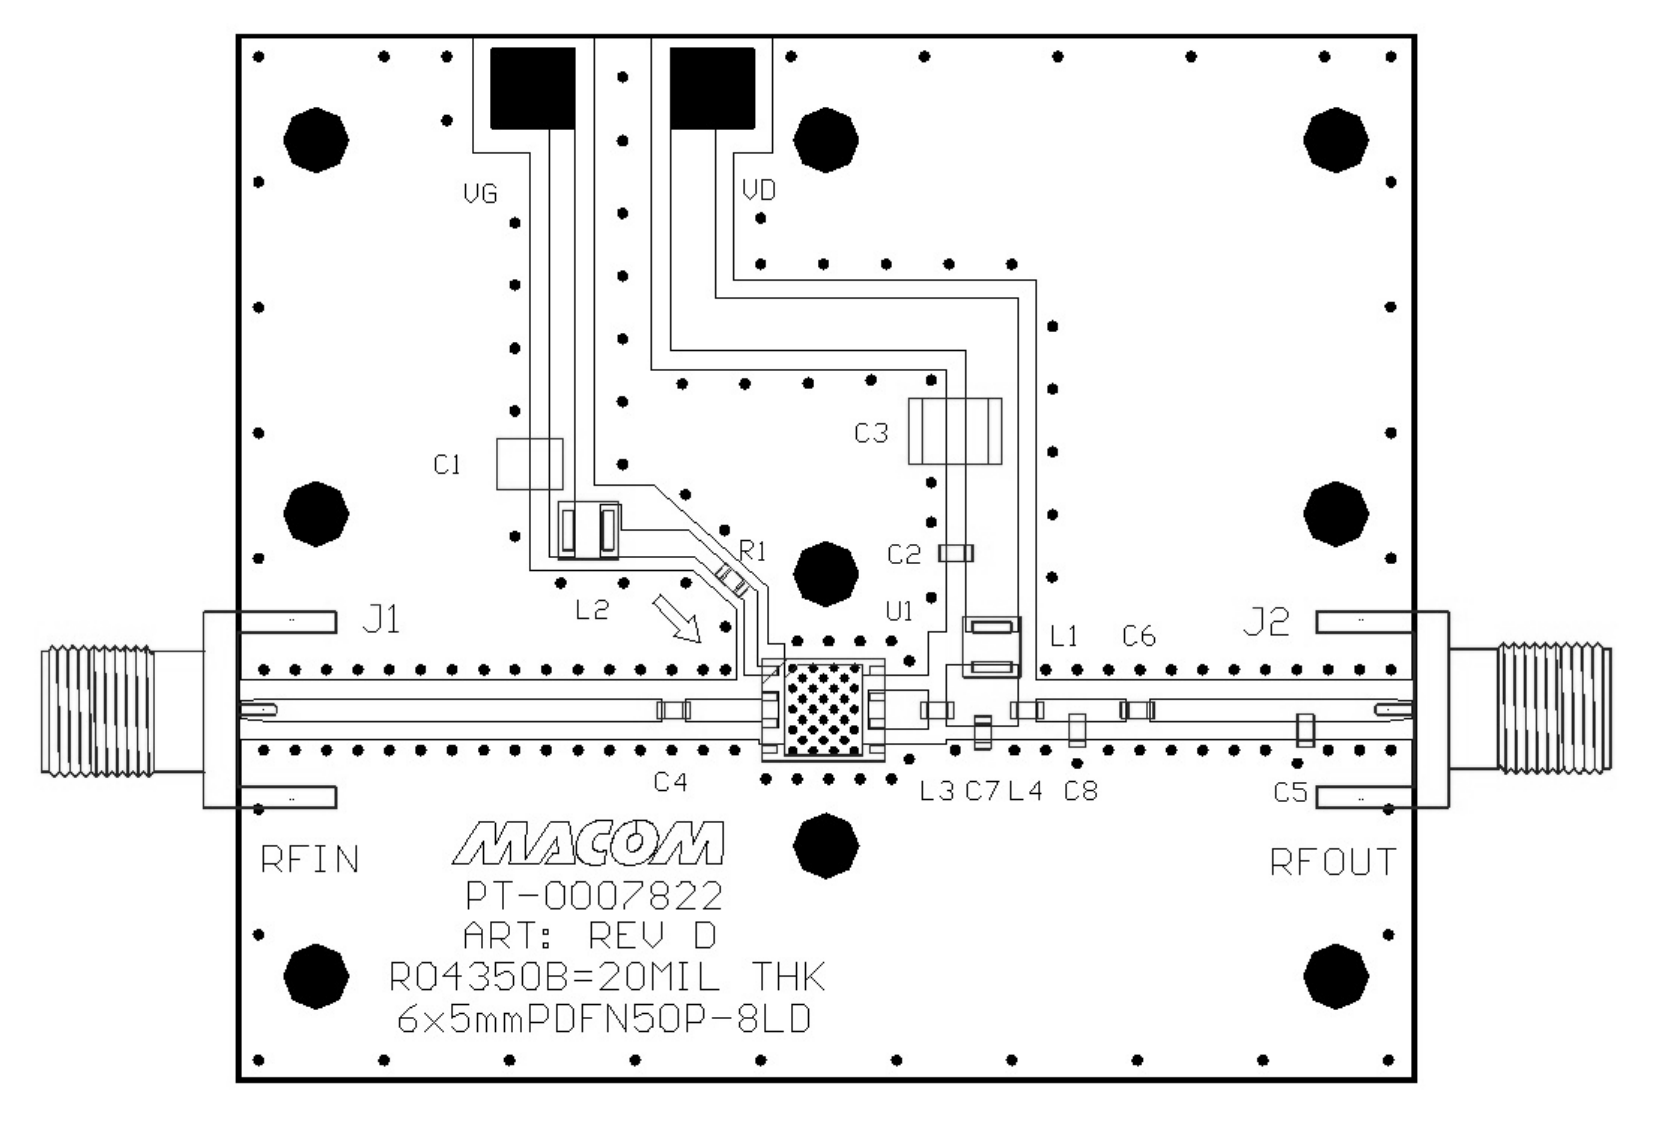
\includegraphics[width=0.9\linewidth]{figs/ch3_NPA1007eval.png}
    \caption{Suggested design for an Evaluation Board from MACOM's NPA1007 \cite{NPA1007}}
    \label{fig:ch3_NPA1007eval.png}
\end{figure}

\par The circuit schematic for the evaluation circuit can be better seen in Figure \ref{fig:ch3_NPA1007schematic.png}. The initial idea would be to utilize the components that are specified by the MACOM. Unfortunately, we were unable to acquire the specified capacitors C5, C7 and C8 sold by Passive Plus (PPI), and those had to be changed for ones that had similar characteristics.

\begin{figure}[H]
    \vspace*{0cm}
    \centering
    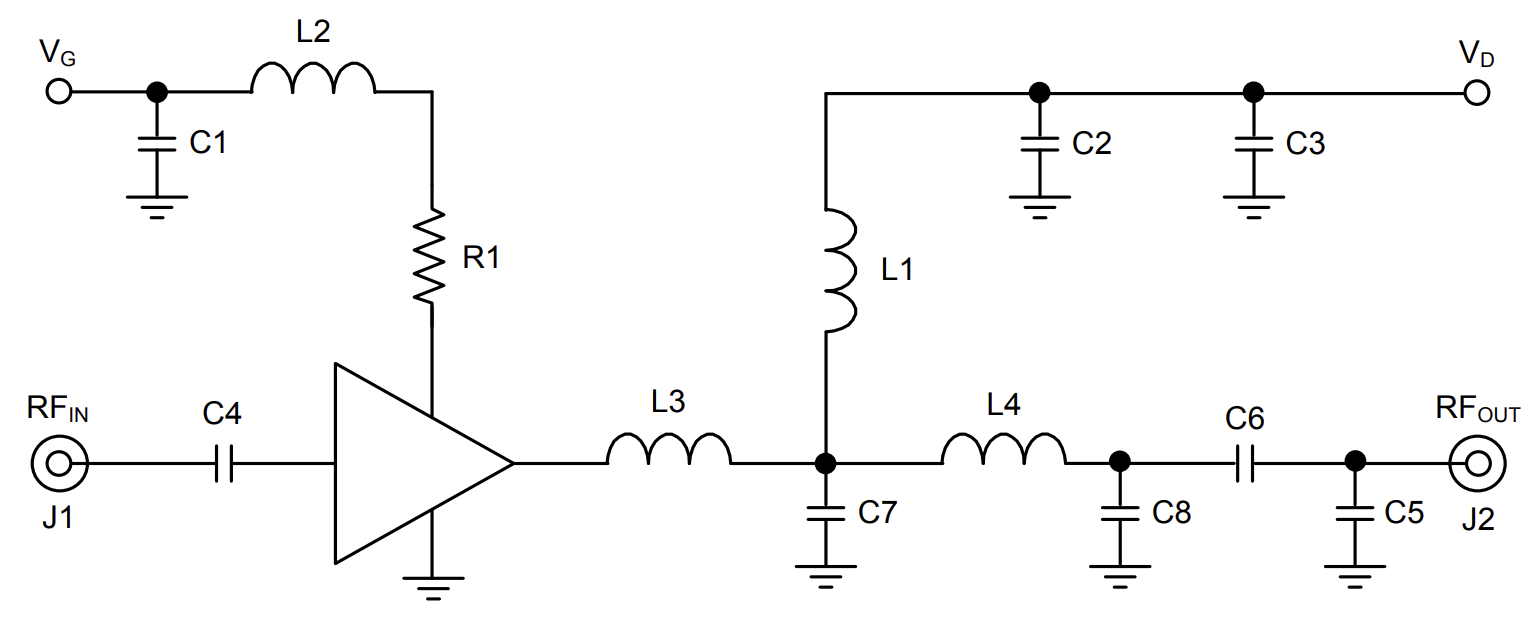
\includegraphics[width=0.9\linewidth]{figs/ch3_NPA1007schematic.png}
    \caption{Schematic for NPA1007 Evaluation Board \cite{NPA1007}}
    \label{fig:ch3_NPA1007schematic.png}
\end{figure}


\par In order to control the gate voltage, a potentiometer should be placed before C1. The chosen potentiometer was a $10\:\si{K\Omega}$, which should be placed as seen in Figure \ref{fig:ch3_NPA1007potentiometer.png}. Unfortunately, during the design of the \ac{pcb}, I mistakenly connected the potentiometer as shown in Figure \ref{fig:ch3_NPA1007potentiometerWRONG.png}. This error prevented the use of the potentiometer to set an adjustable fixed value for $V_{G}$ during the testing phase, as it was essentially a bypass of the potentiometer or the addition of a variable resistance in series with the proposed circuit, depending on how the potentiometer was configured. It made sense to simply bypass the potentiometer and control $V_{G}$ by varying the voltage set on a bench power supply.

\begin{figure}[H]
    \vspace*{0cm}
    \centering
    
\includegraphics[width=0.12\linewidth]{figs/ch3_NPA1007potentiometer.png}
    \caption{Control of $V_{G}$ using a potentiometer corrected}
    \label{fig:ch3_NPA1007potentiometer.png}
\end{figure}

\begin{figure}[H]
    \vspace*{0cm}
    \centering
    
\includegraphics[width=0.15\linewidth]{figs/ch3_NPA1007potentiometerWRONG.png}
    \caption{Control of $V_{G}$ using a potentiometer, using a wrong solution}
    \label{fig:ch3_NPA1007potentiometerWRONG.png}
\end{figure}

\par It was attempted to acquire the models for this component to use in simulations on PathWave ADS, to evaluate the potential behavior of the project. The manufacturer was contacted via e-mail and failed to provide the necessary files to conduct these simulations. After discussing this with Professor Telmo Cunha, the idea of simulating the circuit was then abandoned.

\subsection{Design of the \ac{pcb}}
\par In order to design the \ac{pcb} we first have to understand the internal layout of the case for the circuit. Although the box has a tapering design and the top portion looks larger, from the inside the space is limited by four small plastic bosses where the lid fits in. This means that for a common rectangular \ac{pcb}, its dimensions must be so that it can fit within the space between these bosses. The internal dimensions of the case can be seen in Figure \ref{fig:ch3_CU-793-MBinternal.png} present in its datasheet.

\begin{figure}[H]
    \vspace*{0cm}
    \centering
    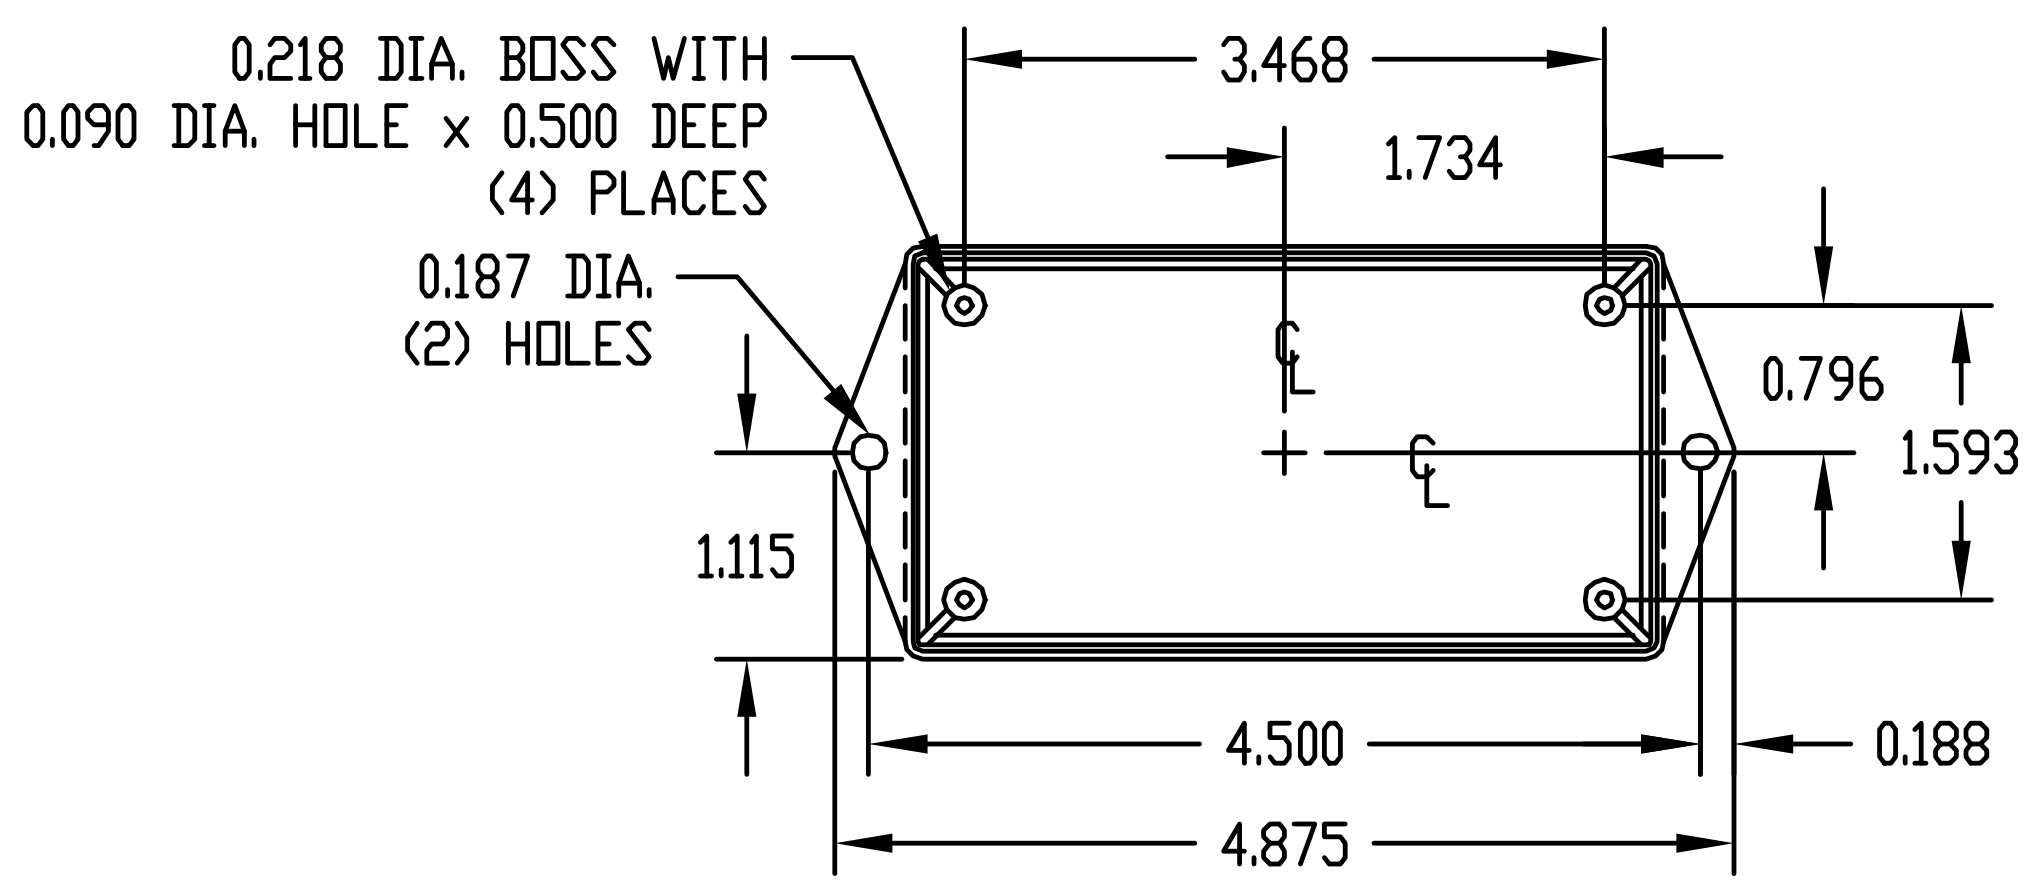
\includegraphics[width=0.7\linewidth]{figs/ch3_CU-793-MBinternal.png}
    \caption{Internal dimension of the CU-793-MB case \cite{UtiliboxCUR-793}}
    \label{fig:ch3_CU-793-MBinternal.png}
\end{figure}

\par So, in order to fit inside the case, our \ac{pcb} has to have a maximum width of $3.49 \:\si{cm}$ and length of $8.28 \:\si{cm}$. These restrictions made it impossible to fit the whole project in a single \ac{pcb} while trying to keep all components in the same layer, as the circuit that we planned to use for the \acl{pa} would occupy a significant portion of the layout. As such, it was devised that the circuit would be divided into two \ac{pcb}. The first, larger one would incorporate the majority of the components, and also all the inputs for the prototype. The second would be only for the \ac{pa} portion with its potentiometer and the circulator.

\par This meant that there had to be a way of maintaining the two different \ac{pcb} in position inside the case without touching each other. For this problem we figured that they could be kept separated if we used plastic washers placed between them. For this, we would leave three holes on each \ac{pcb}, where plastic studs could be inserted. The \ac{pcb} would be placed with their bottom layers facing each other and the top layers facing out. In this way there would be no chance of an accidental contact between their components, and we would not have any clearance problems related to component heights.

\par This approach is not without faults. There is now a need to pass both the $28\:\si{V}$, $-5\:\si{V}$, GND and the \ac{rf} signal that exits the driver amplifier to the second \ac{pcb}. For the DC signals and GND, common wires were used, in order to connect these signals. The driver would connect to the \ac{pa} via a small portion of coxial cable. Although the coaxial cable would already provide a suitable GND connection between both \ac{pcb}, we still used a wire connection.

\par In order to create the \ac{pcb}s, the footprints and models for the components when the manufacturer does not provide them, EAGLE from Autodesk was used. The bigger board has a length of $8\:\si{cm}$ and a width of $4\:\si{cm}$. This allows the board to sit inside the space created by the bosses. Although the width is bigger, this is by design as it does not allow movement of the board in at least one of the axes if it became loose. The final design of this board can be seen in Figure \ref{fig:ch3_PCBlayout1.png}.

\begin{figure}[H]
    \vspace*{0cm}
    \centering
    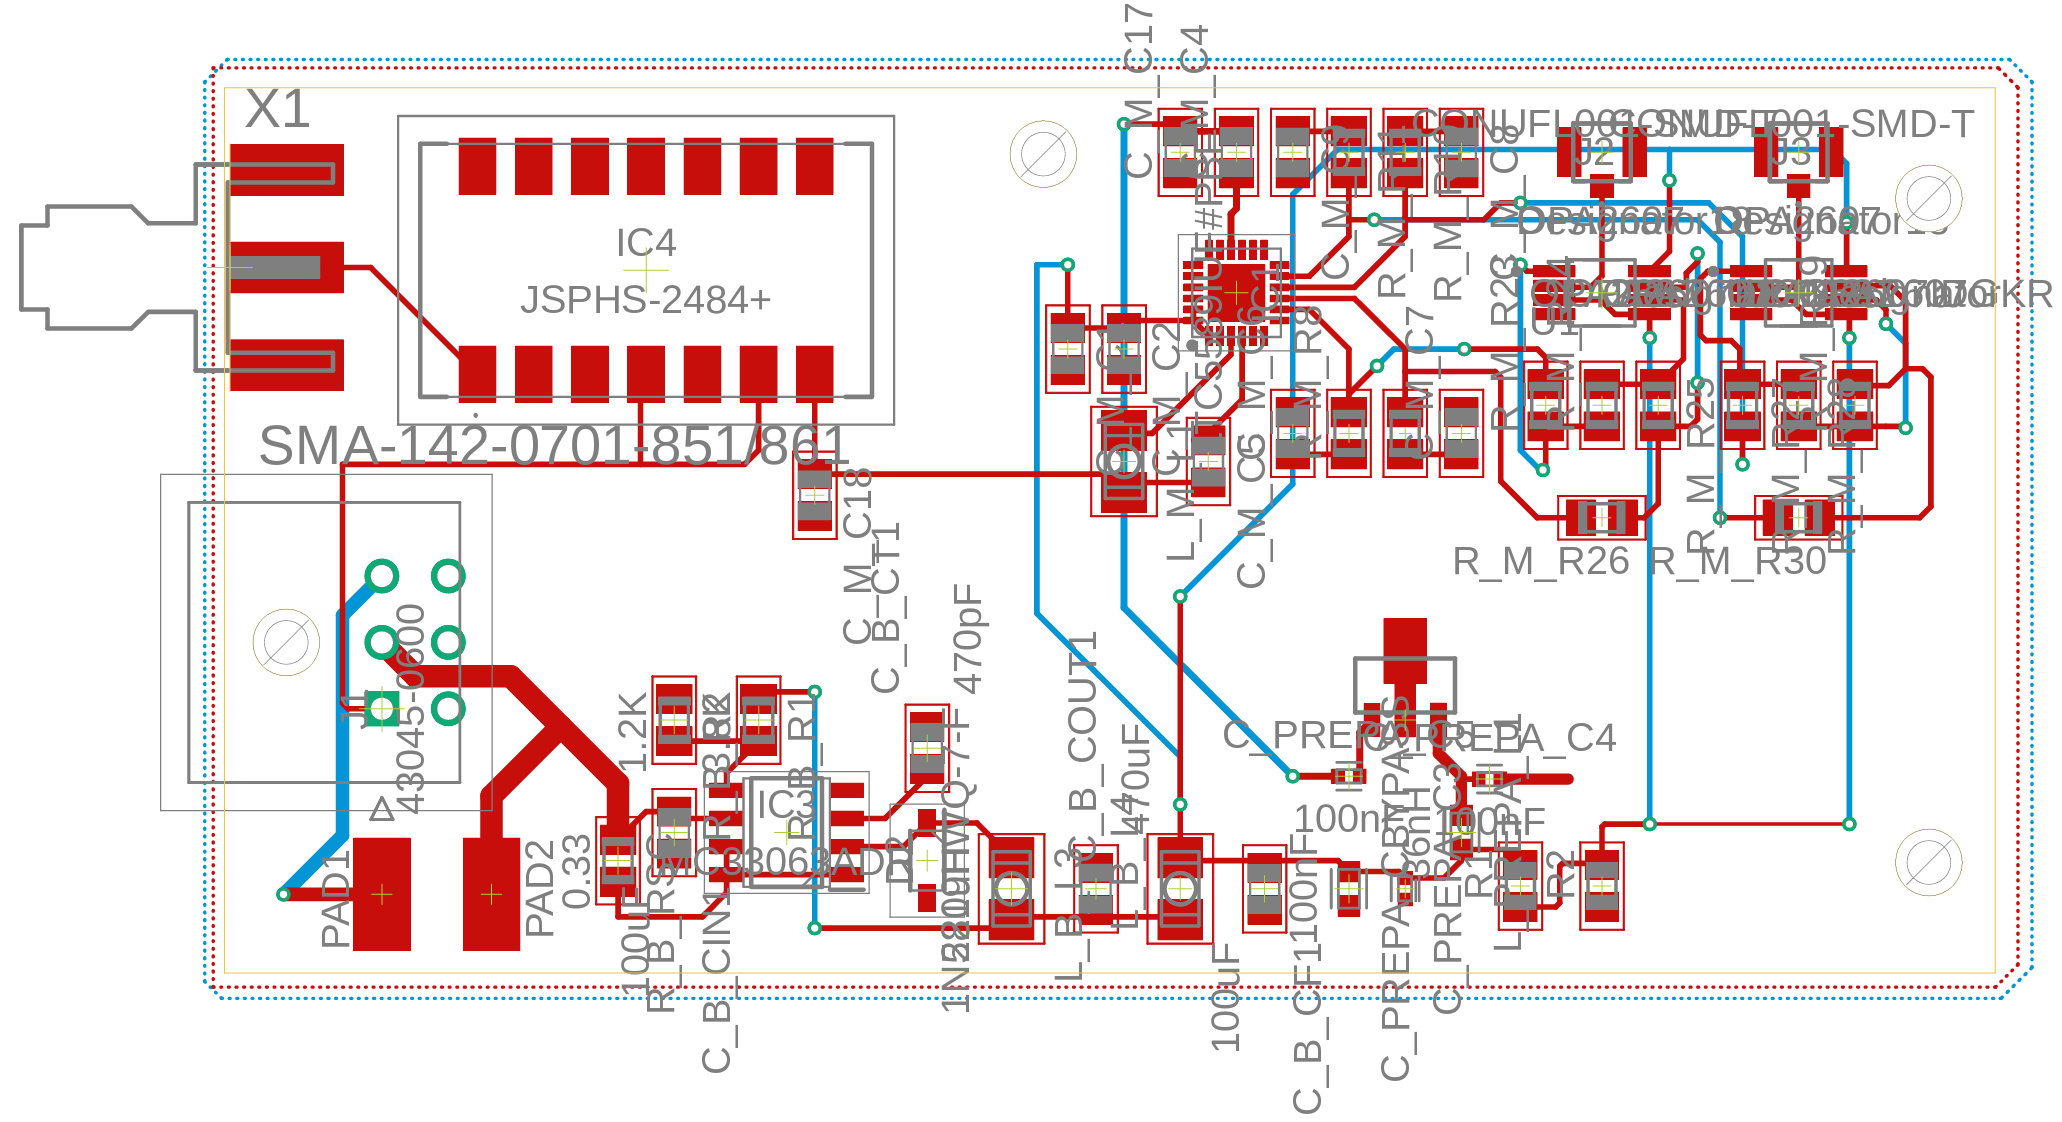
\includegraphics[width=0.8\linewidth]{figs/ch3_PCBlayout1.png}
    \caption{First \ac{pcb}}
    \label{fig:ch3_PCBlayout1.png}
\end{figure}

\par The three holes that were left in order to keep the board in position have a drill size of $3\:\si{mm}$ on EAGLE. These were positioned on both boards away so that they can be placed back-to-back. 

\par The \ac{pcb} for the \ac{pa} portion of the project has a smaller size, totaling $6\:\si{cm}$ in length and $4\:\si{cm}$ in width. On the second board, which contains the \ac{pa}, shown in Figure \ref{fig:ch3_PCBlayout1.png} we also added several through-hole vias that connect both sides of the board. This helps to distribute the heat that can be generated during operation. It should be noted, once again, that the connections to the potentiometer are wrong. This has been addressed earlier in the document.

\begin{figure}[H]
    \vspace*{0cm}
    \centering
    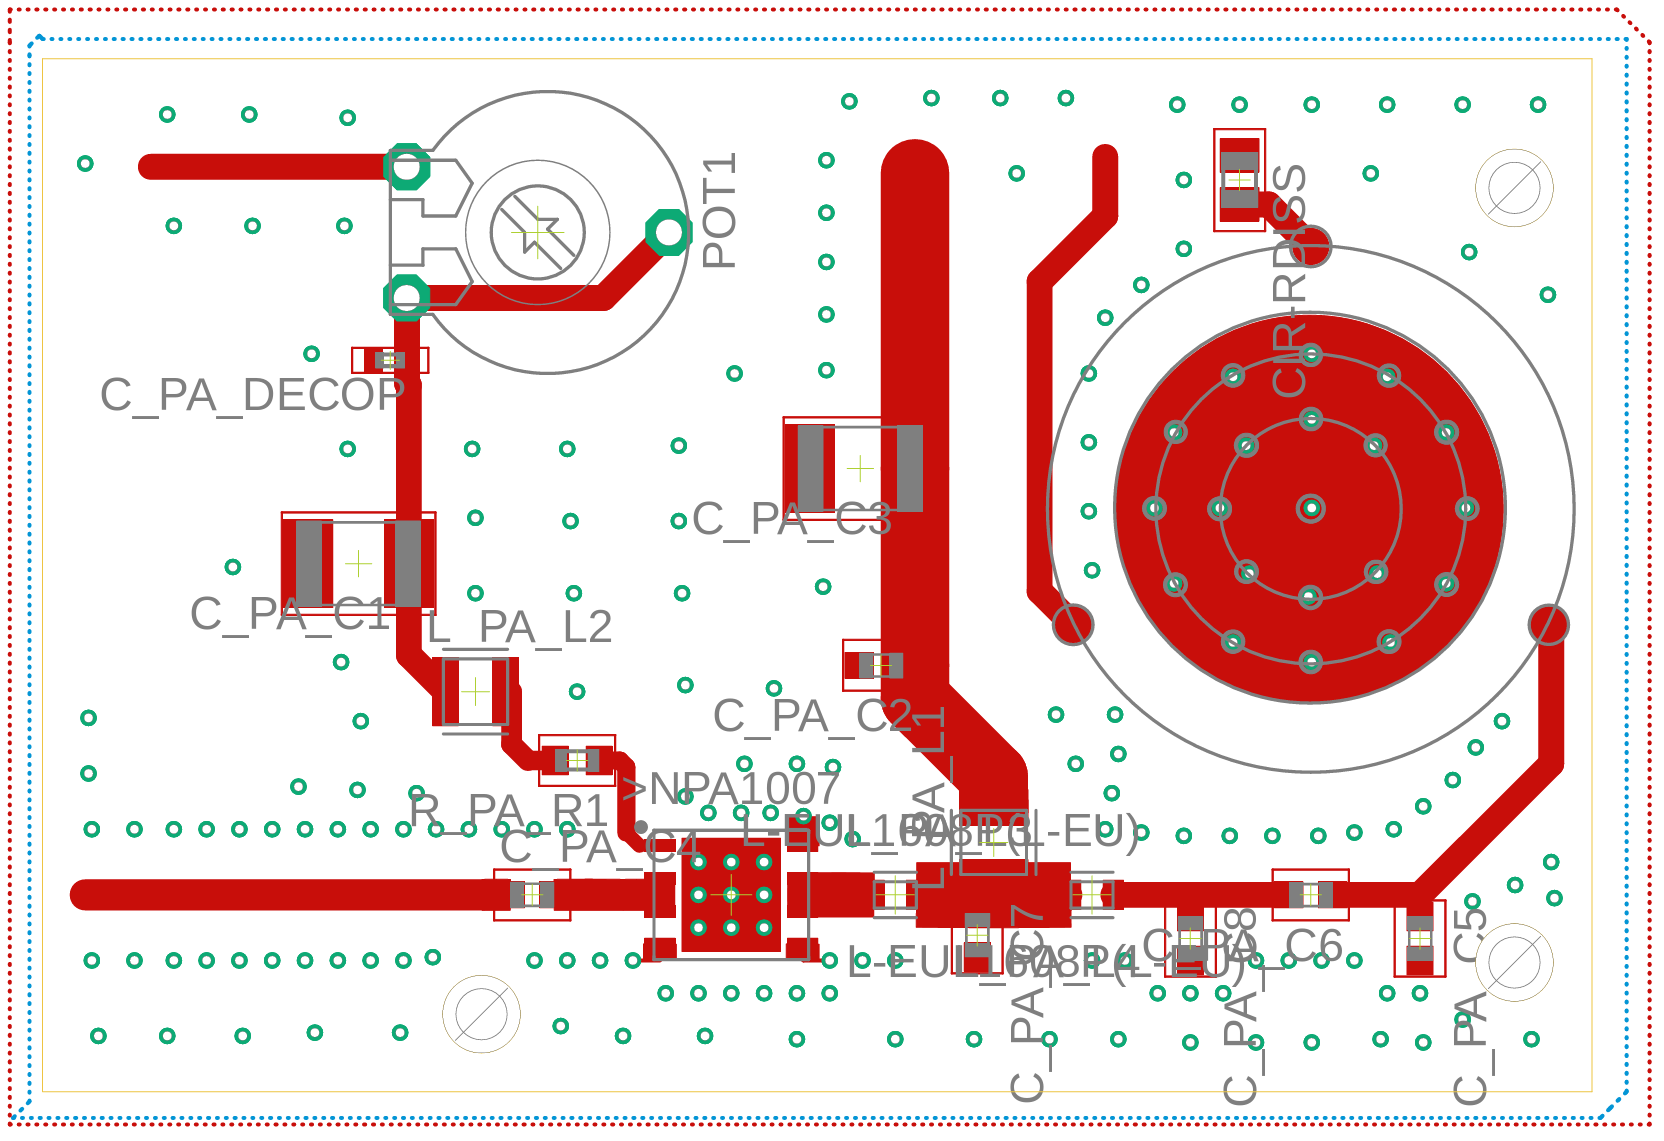
\includegraphics[width=0.8\linewidth]{figs/ch3_PCBlayout2.png}
    \caption{Second \ac{pcb}}
    \label{fig:ch3_PCBlayout2.png}
\end{figure}

\par It should be added that, although not entirely obvious from Figures \ref{fig:ch3_PCBlayout1.png} and \ref{fig:ch3_PCBlayout2.png}, both \ac{pcb} designs contain copper pours on the top and bottom layers. These are connected directly to GND.

\section{Spiral Antenna Design}
\par These types of antenna are characterized by their ability to have a consistence impedance and radiation pattern across a broad range of frequencies \cite{ConstantineA.Balanis2016AntennaDesign}. These antennas can have more than one arm, turning around itself forming a spiral. 

\par As they tend to generally have smaller sizes and respectable bandwidth, these can be used for application in broadband communication systems.

\par Spiral antennas operate by having resonance to different frequencies on different parts of the spiral, or spirals, that comprise them. Their design involves considering factors such as width of the arms or the spacing between them, the number of turns, and overall size of the antenna itself.

\par There are three main types of spiral antennas: archimedean, equiangular and logarithmic. For this project the focus was to create an archimedean type spiral antenna, having constant spacing between the two arms. In the end, after using Dassault Systems' CST Studio Suite to help with the design, our antenna was more of a logarithmic, with variable spacing between arms.

\par One characteristic of spiral antennas, and one that is a concern in this application, is that they radiate towards both sides. This means that if the antenna is in the front side of the box and radiates one of its two main lobes towards the intended location, there will inevitably be another main lobe in the opposite direction. 

\par This would not bode well for the operation of the array element, as it would be subject to a rather large power \ac{rf} signal potentially causing malfunction of the circuit and the equipment.

\par To prevent this problem, a box made of \ac{pcb} can be constructed around the antenna back, to protect the circuits behind it. This box will have a depth of around a quarter-wavelength of the desired carrier frequency. Theoretically, this depth would have been of $31.25\:\si{mm}$. This outer box is not connected to ground. This makes it so that any possible reflection would be canceled. 

\par In order to feed signal to the antenna, a front panel female SMA  connector is placed on the external part of the antenna box. To bridge the interior gap of the box, a small length of coaxial cable was used. This cable would then go through two small holes in the antenna arms to establish a connection.

\par The initial idea for the design of the antenna is explained by \citet{Caswell2002DesignSizes} on his PhD Thesis. Here, it is explained that the outer radius of the antenna, $R_{OUTER}$ can be calculated through (\ref{eq:ch3_outerRadius}). This dimension is directly related to the lowest frequency, $f_{LOW}$ of the desired range, because the lowest frequency at which the antenna resonates will have the longest wavelength.

\begin{equation}
    \label{eq:ch3_outerRadius}
    R_{OUTER} = \frac{c}{2\cdot f_{LOW}\cdot\pi}
\end{equation}

\par The inner radius of the antenna is calculated using Equation \ref{eq:ch3_innerRadius}. Because this length is related to the minimum wavelength at which the antenna will be able to resonate at, this sets the maximum frequency of the antenna, $f_{HIGH}$.

\begin{equation}
    \label{eq:ch3_innerRadius}
    R_{INNER} = \frac{c}{2\cdot f_{HIGH}\cdot\pi}
\end{equation}

\par The process of calculating the spacing between the arms, $S$, and the width of this arms, $W$, is explained by \cite{Caswell2002DesignSizes}. These two dimensions are the same for an archimedean antenna, as shown by Equation (\ref{eq:ch3_SandW}). In this equation $N$ refers to the number of turns of the antenna arms.

\begin{equation}
    \label{eq:ch3_SandW}
    s = w = \frac{r_{OUTER}-r_{INNER}}{4\cdot N}
\end{equation}

\par If we want to use these equations for an antenna with $N = 3.5$ that covers the interval from $1.8\:\si{GHz}$ to $5\:\si{GHz}$, we arrive at values for $R_{INNER} = 9.5\:\si{mm}$ and $R_{OUTER} = 2.7\:\si{cm}$, with a width and spacing of $1.18\:\si{mm}$.

\par We can fit the arms of such an antenna in a $5\:\si{cm}$ by $5\:\si{cm}$ square of substrate. The only problem is that we are going to have to angle this antenna so that the tips of its arms are at a corner rather than in the middle section of the square side. The substrate used for the antenna was RO4350B, while the one used for the box is FR-4.

\par The initial simulation performed in CST Studio for an antenna with these dimensions produced results that were not ideal for an antenna operating at a frequency of $2.4\:\si{GHz}$. Therefore, a process of iterative tuning of the parameters of the antenna was conducted within CST Studio.

\par In the end, we ended up with arms that were based on the lines with the equations that are shown on Figure \ref{fig:ch3_Spiral.png}.

\begin{figure}[H]
    \vspace*{0cm}
    \centering
    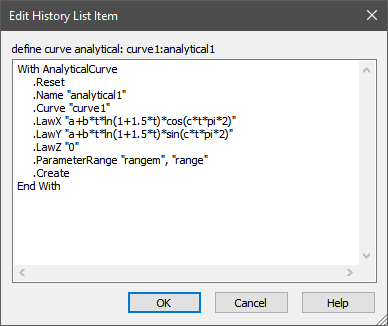
\includegraphics[width=0.5\linewidth]{figs/ch3_Spiral.png}
    \caption{Parameters for the line defining the arms}
    \label{fig:ch3_Spiral.png}
\end{figure}

\par After a long iterative optimization process, we arrived at an antenna that is shown in Figure \ref{fig:ch3_antenna.PNG}

\begin{figure}[H]
    \vspace*{0cm}
    \centering
    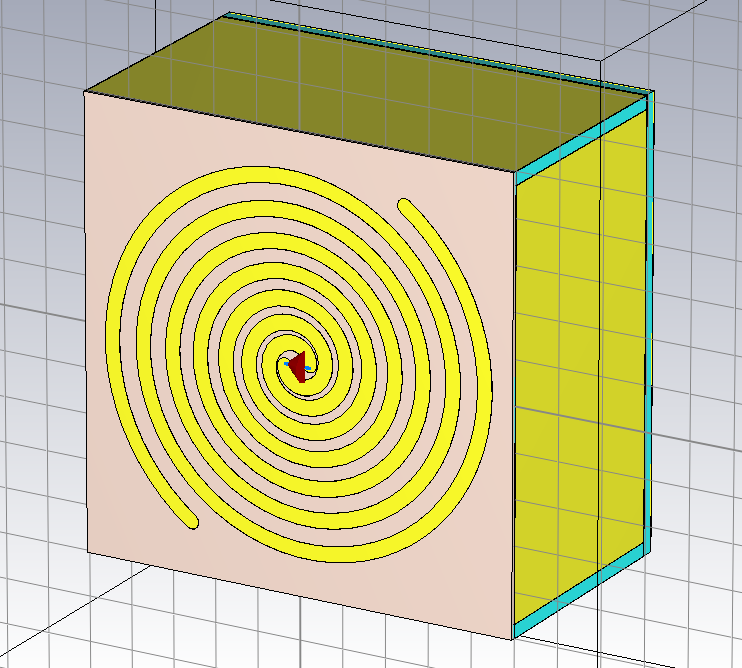
\includegraphics[width=0.5\linewidth]{figs/ch3_antenna.PNG}
    \caption{Antenna obtained on CST Studio}
    \label{fig:ch3_antenna.PNG}
\end{figure}

\par The dimensions of the antenna can be seen in Figure \ref{fig:ch3_parameter_list.PNG}. Here, "subsW" is the width of the antenna and "subsL" is its length. The parameters "subsTantenna" and "copperT" refer to characteristics of the substrate RO4350B, being both its thickness of the actual substrate and the thickness of the copper, respectively. The parameter "boxDepth" refers to the internal distance between the antenna and the opposite side of the box. The thickness of each side of the box is "subsT". All the other parameters help to control how the antenna's arms look. Both "rangem" and "a" help to indicate where the arms would start near the center. To control how closer the arms are to each other, "c" and "b" were used. To control the number of turns for each arm, we used the value of "range".

\begin{figure}[H]
    \vspace*{0cm}
    \centering
    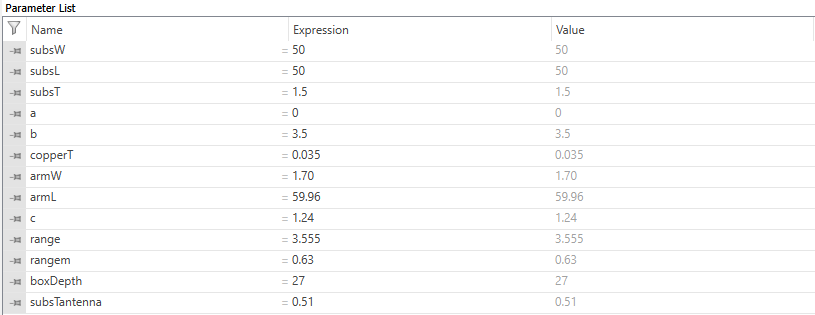
\includegraphics[width=0.9\linewidth]{figs/ch3_parameter_list.PNG}
    \caption{Parameter list for the construction and simulation of the antenna.}
    \label{fig:ch3_parameter_list.PNG}
\end{figure}

\par The obtained antenna performance can be seen in the next images. Figure \ref{fig:ch3_s11.png} shows the input reflection coefficient of the antenna. Although during the simulations performed on CST Studio the lowest value of S11 was not located at the frequency of $2.4\:\si{GHz}$, the antenna still had a decent reflection coefficient at that frequency. And with the certainty that when printed the physical antenna would not retain the same S11 parameter shown in CST Studio, we felt comfortable enough to use this design. 

\begin{figure}[H]
    \vspace*{0cm}
    \centering
    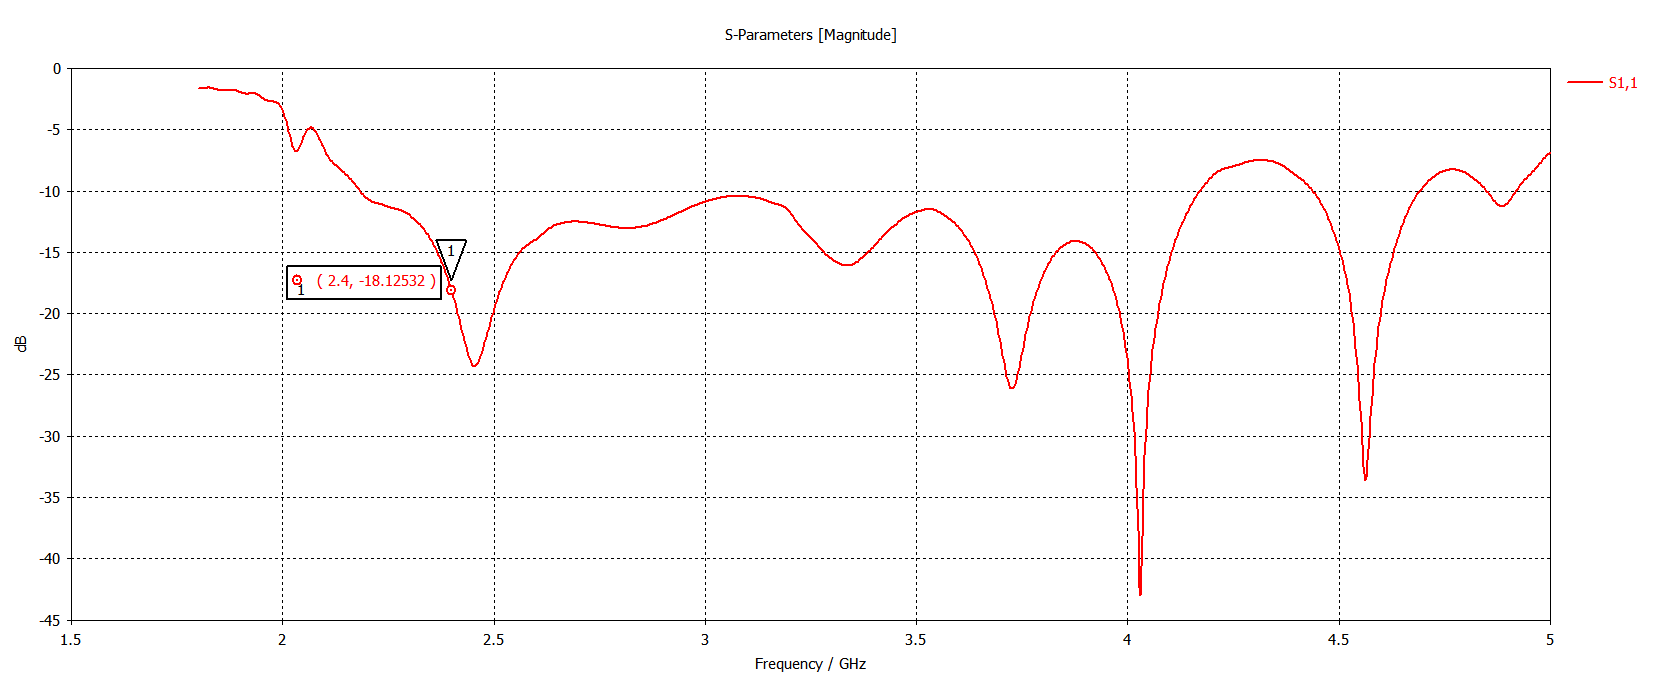
\includegraphics[width=0.9\linewidth]{figs/ch3_s11.png}
    \caption{VSWR of the antenna over frequency}
    \label{fig:ch3_s11.png}
\end{figure}

\par We can also observe the antenna's simulated VSWR in Figure \ref{fig:ch3_VSWR.png}, which is about $1.28$ for the desired frequency.

\begin{figure}[H]
    \vspace*{0cm}
    \centering
    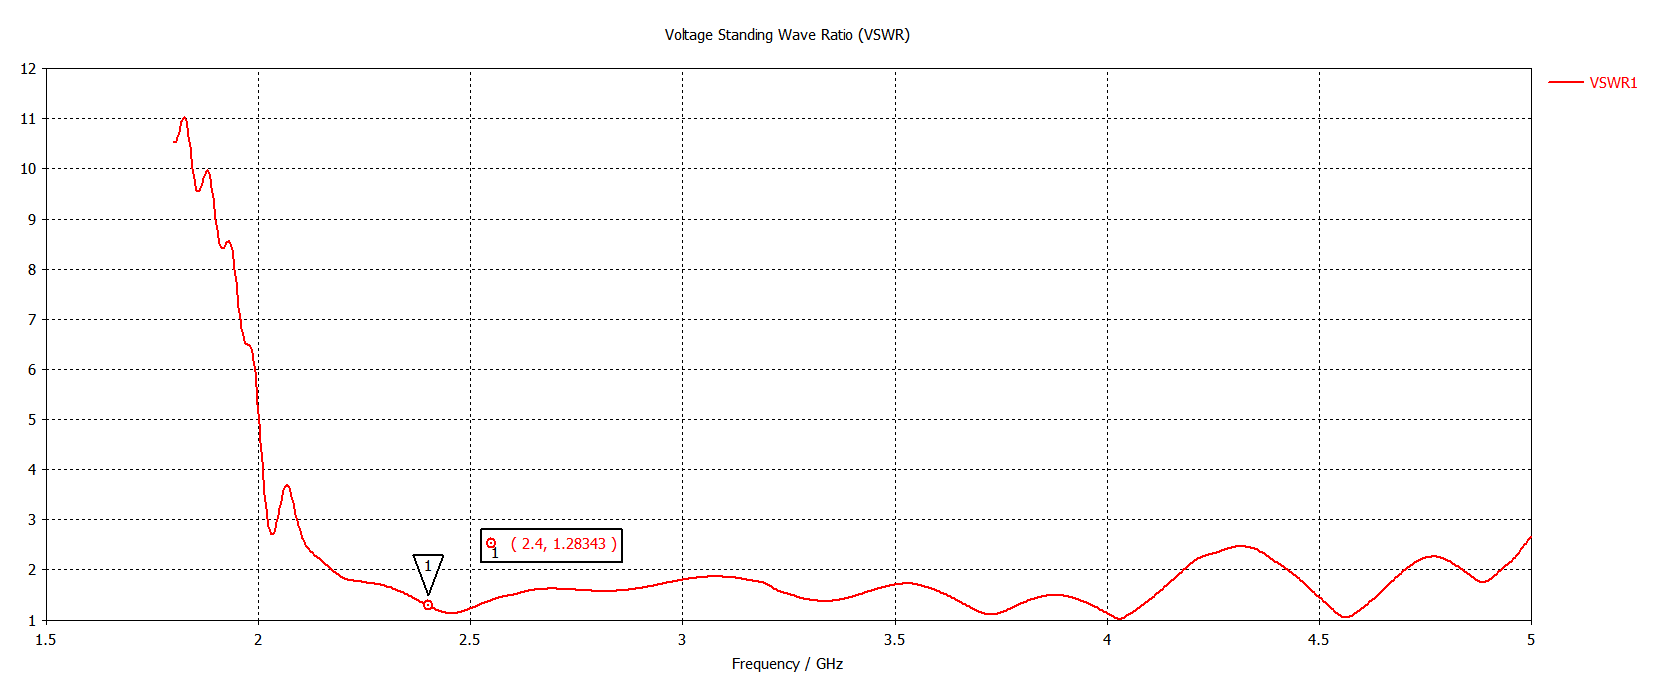
\includegraphics[width=0.9\linewidth]{figs/ch3_VSWR.png}
    \caption{VSWR of the antenna over frequency}
    \label{fig:ch3_VSWR.png}
\end{figure}

\par The Figures \ref{fig:ch3_farfield.PNG} and \ref{fig:ch3_farfieldBack.png} help visualize the form of the antenna radiation pattern. As we can see, the antenna does have good directivity coming in at $6.186\:\si{dBi}$ for the front, and being able to have a reduced value for the back. This helps understand better the effects of the box on the radiation pattern of the antenna.

\begin{figure}[H]
    \vspace*{0cm}
    \centering
    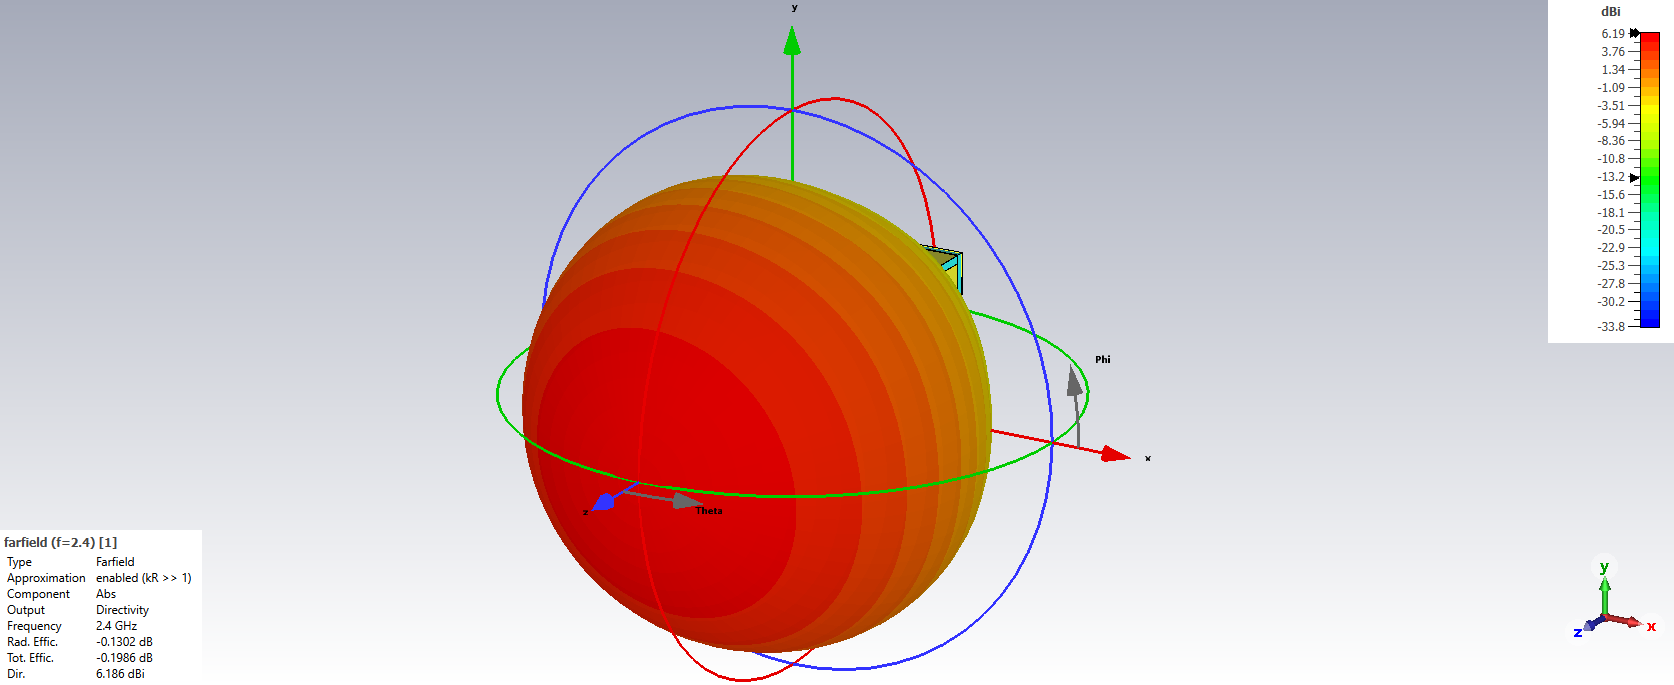
\includegraphics[width=0.9\linewidth]{figs/ch3_farfield.png}
    \caption{Front facing directivity}
    \label{fig:ch3_farfield.PNG}
\end{figure}

\begin{figure}[H]
    \vspace*{0cm}
    \centering
    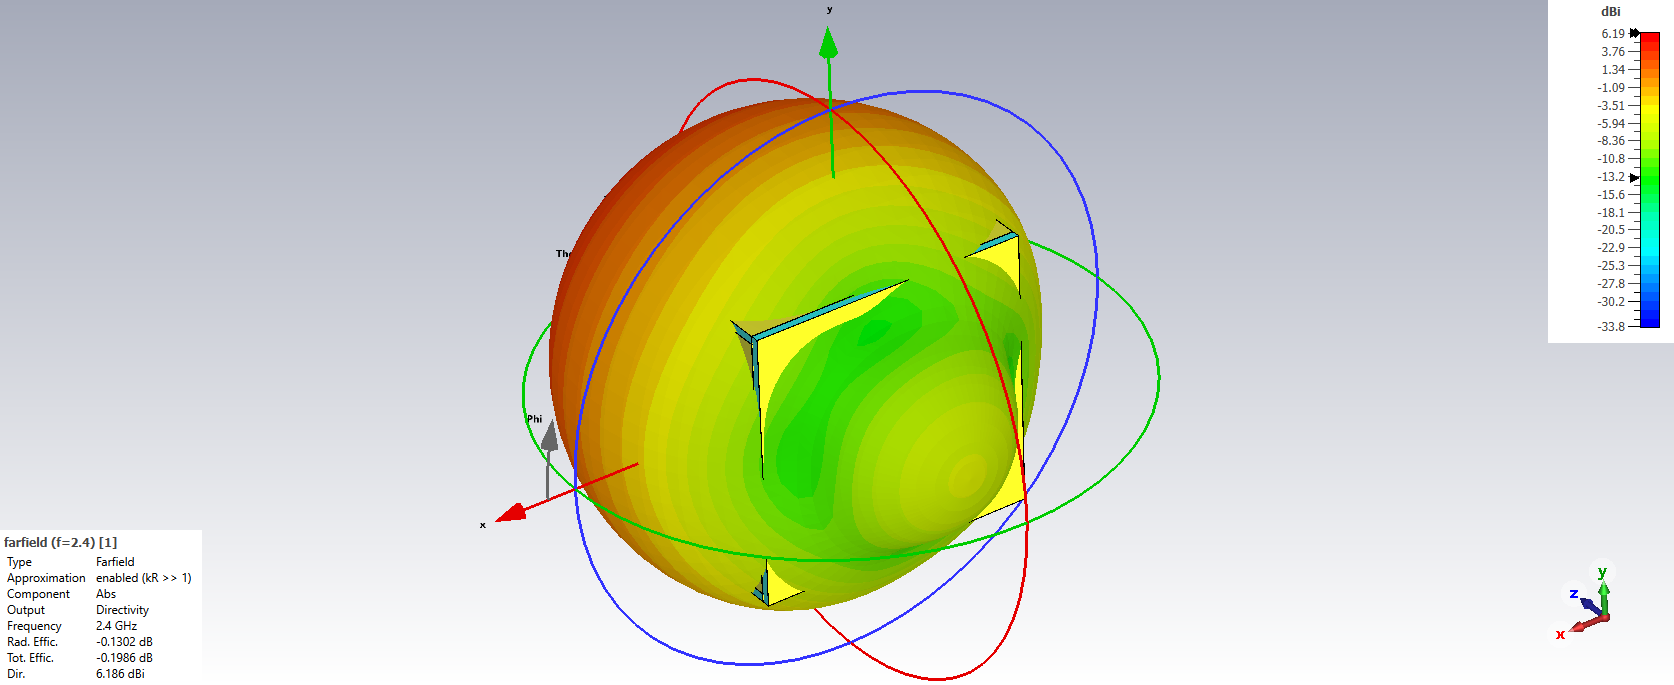
\includegraphics[width=0.9\linewidth]{figs/ch3_farfieldBack.png}
    \caption{Back facing directivity}
    \label{fig:ch3_farfieldBack.png}
\end{figure}

\par A better way to observe the farfield directivity of the antenna is through Figure \ref{fig:ch3_farfield1D.png}. Here, we can see the body of the antenna, as well as how it is radiating. We can also see that in simulation there is an offset of 2º on the main lobe direction of the antenna.

\begin{figure}[H]
    \vspace*{0cm}
    \centering
    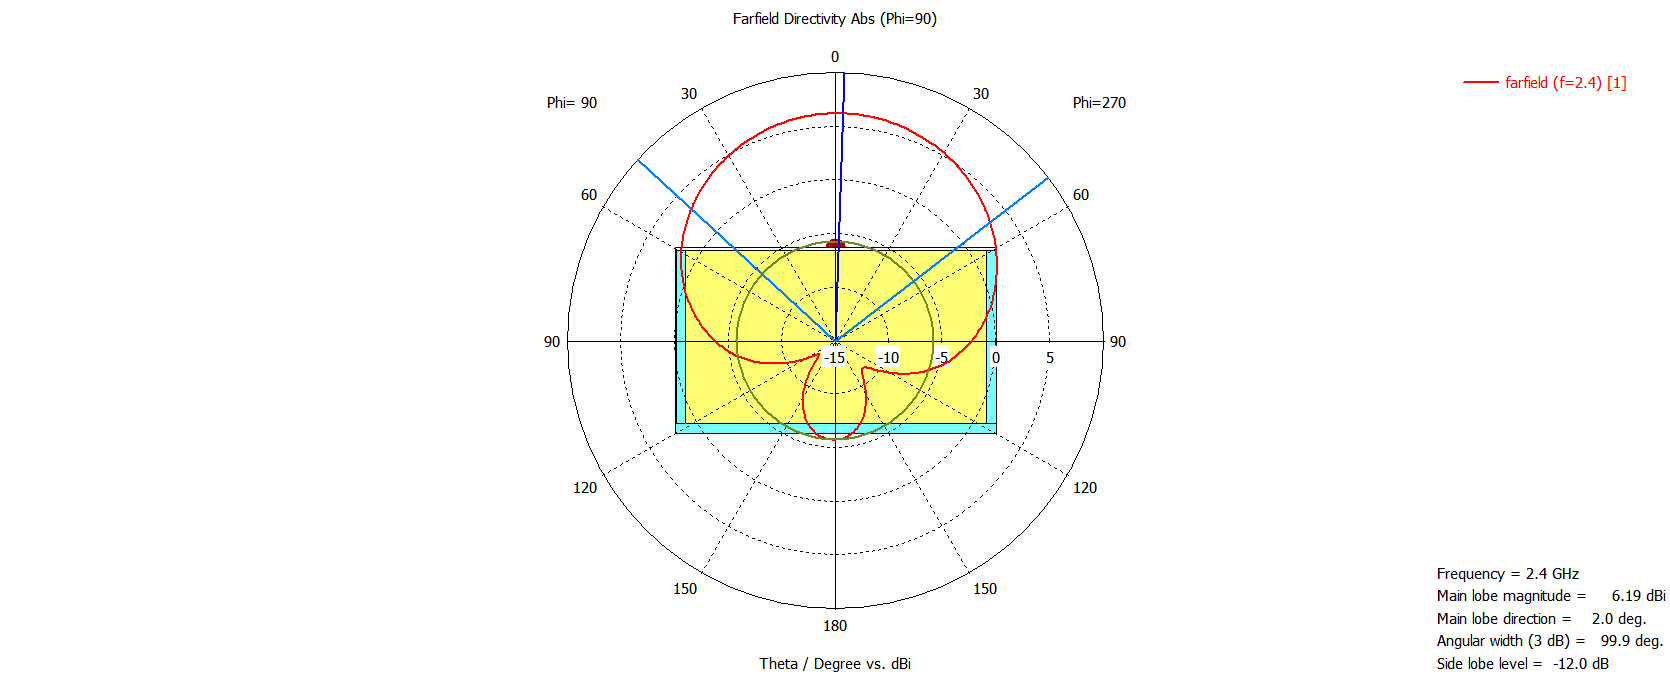
\includegraphics[width=0.9\linewidth]{figs/ch3_farfield1D.png}
    \caption{Farlfield directivity in 1D for Phi = 90}
    \label{fig:ch3_farfield1D.png}
\end{figure}

\par The gain of the antenna, as described by IEEE, is shown on Figure \ref{fig:ch3_gain.png}. We can see that its front facing gain, at $0^{\circ}$, is of $6.07\:\si{dB}$, and that it can attenuate the signal to the back, $180^{\circ}$, having a gain of $-5.90\:\si{dB}$.

\begin{figure}[H]
    \vspace*{0cm}
    \centering
    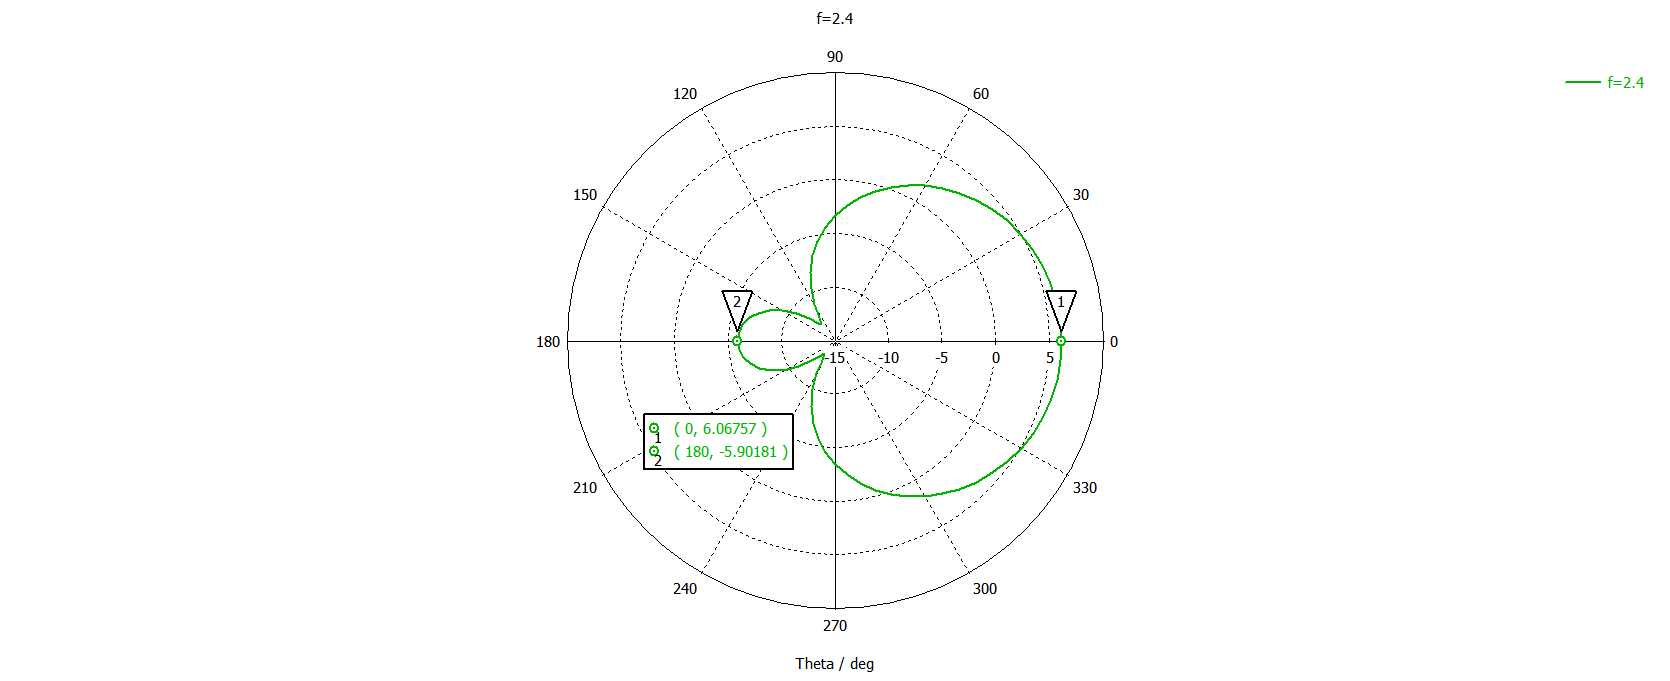
\includegraphics[width=0.9\linewidth]{figs/ch3_gain.png}
    \caption{Farlfield directivity in 1D for Phi = 90}
    \label{fig:ch3_gain.png}
\end{figure}

\par Afterwards, we decided to print two antennas. Instead of assembling both antennas at the same time, it was decided to do one at a time. The first was antenna 1 and the second was antenna 2. Both antennas were printed according to the same specifications. The box behind each antenna was also built according to the same dimensions. This eventually allowed us to improve antenna 2 based on the measurements of antenna 1.

\par The box from antenna 1 was made by soldering the sides of the box only on the corners, as can be seen on Figure \ref{fig:ch3_antenna1Box.jpg}. 

\begin{figure}[H]
    \vspace*{0cm}
    \centering
    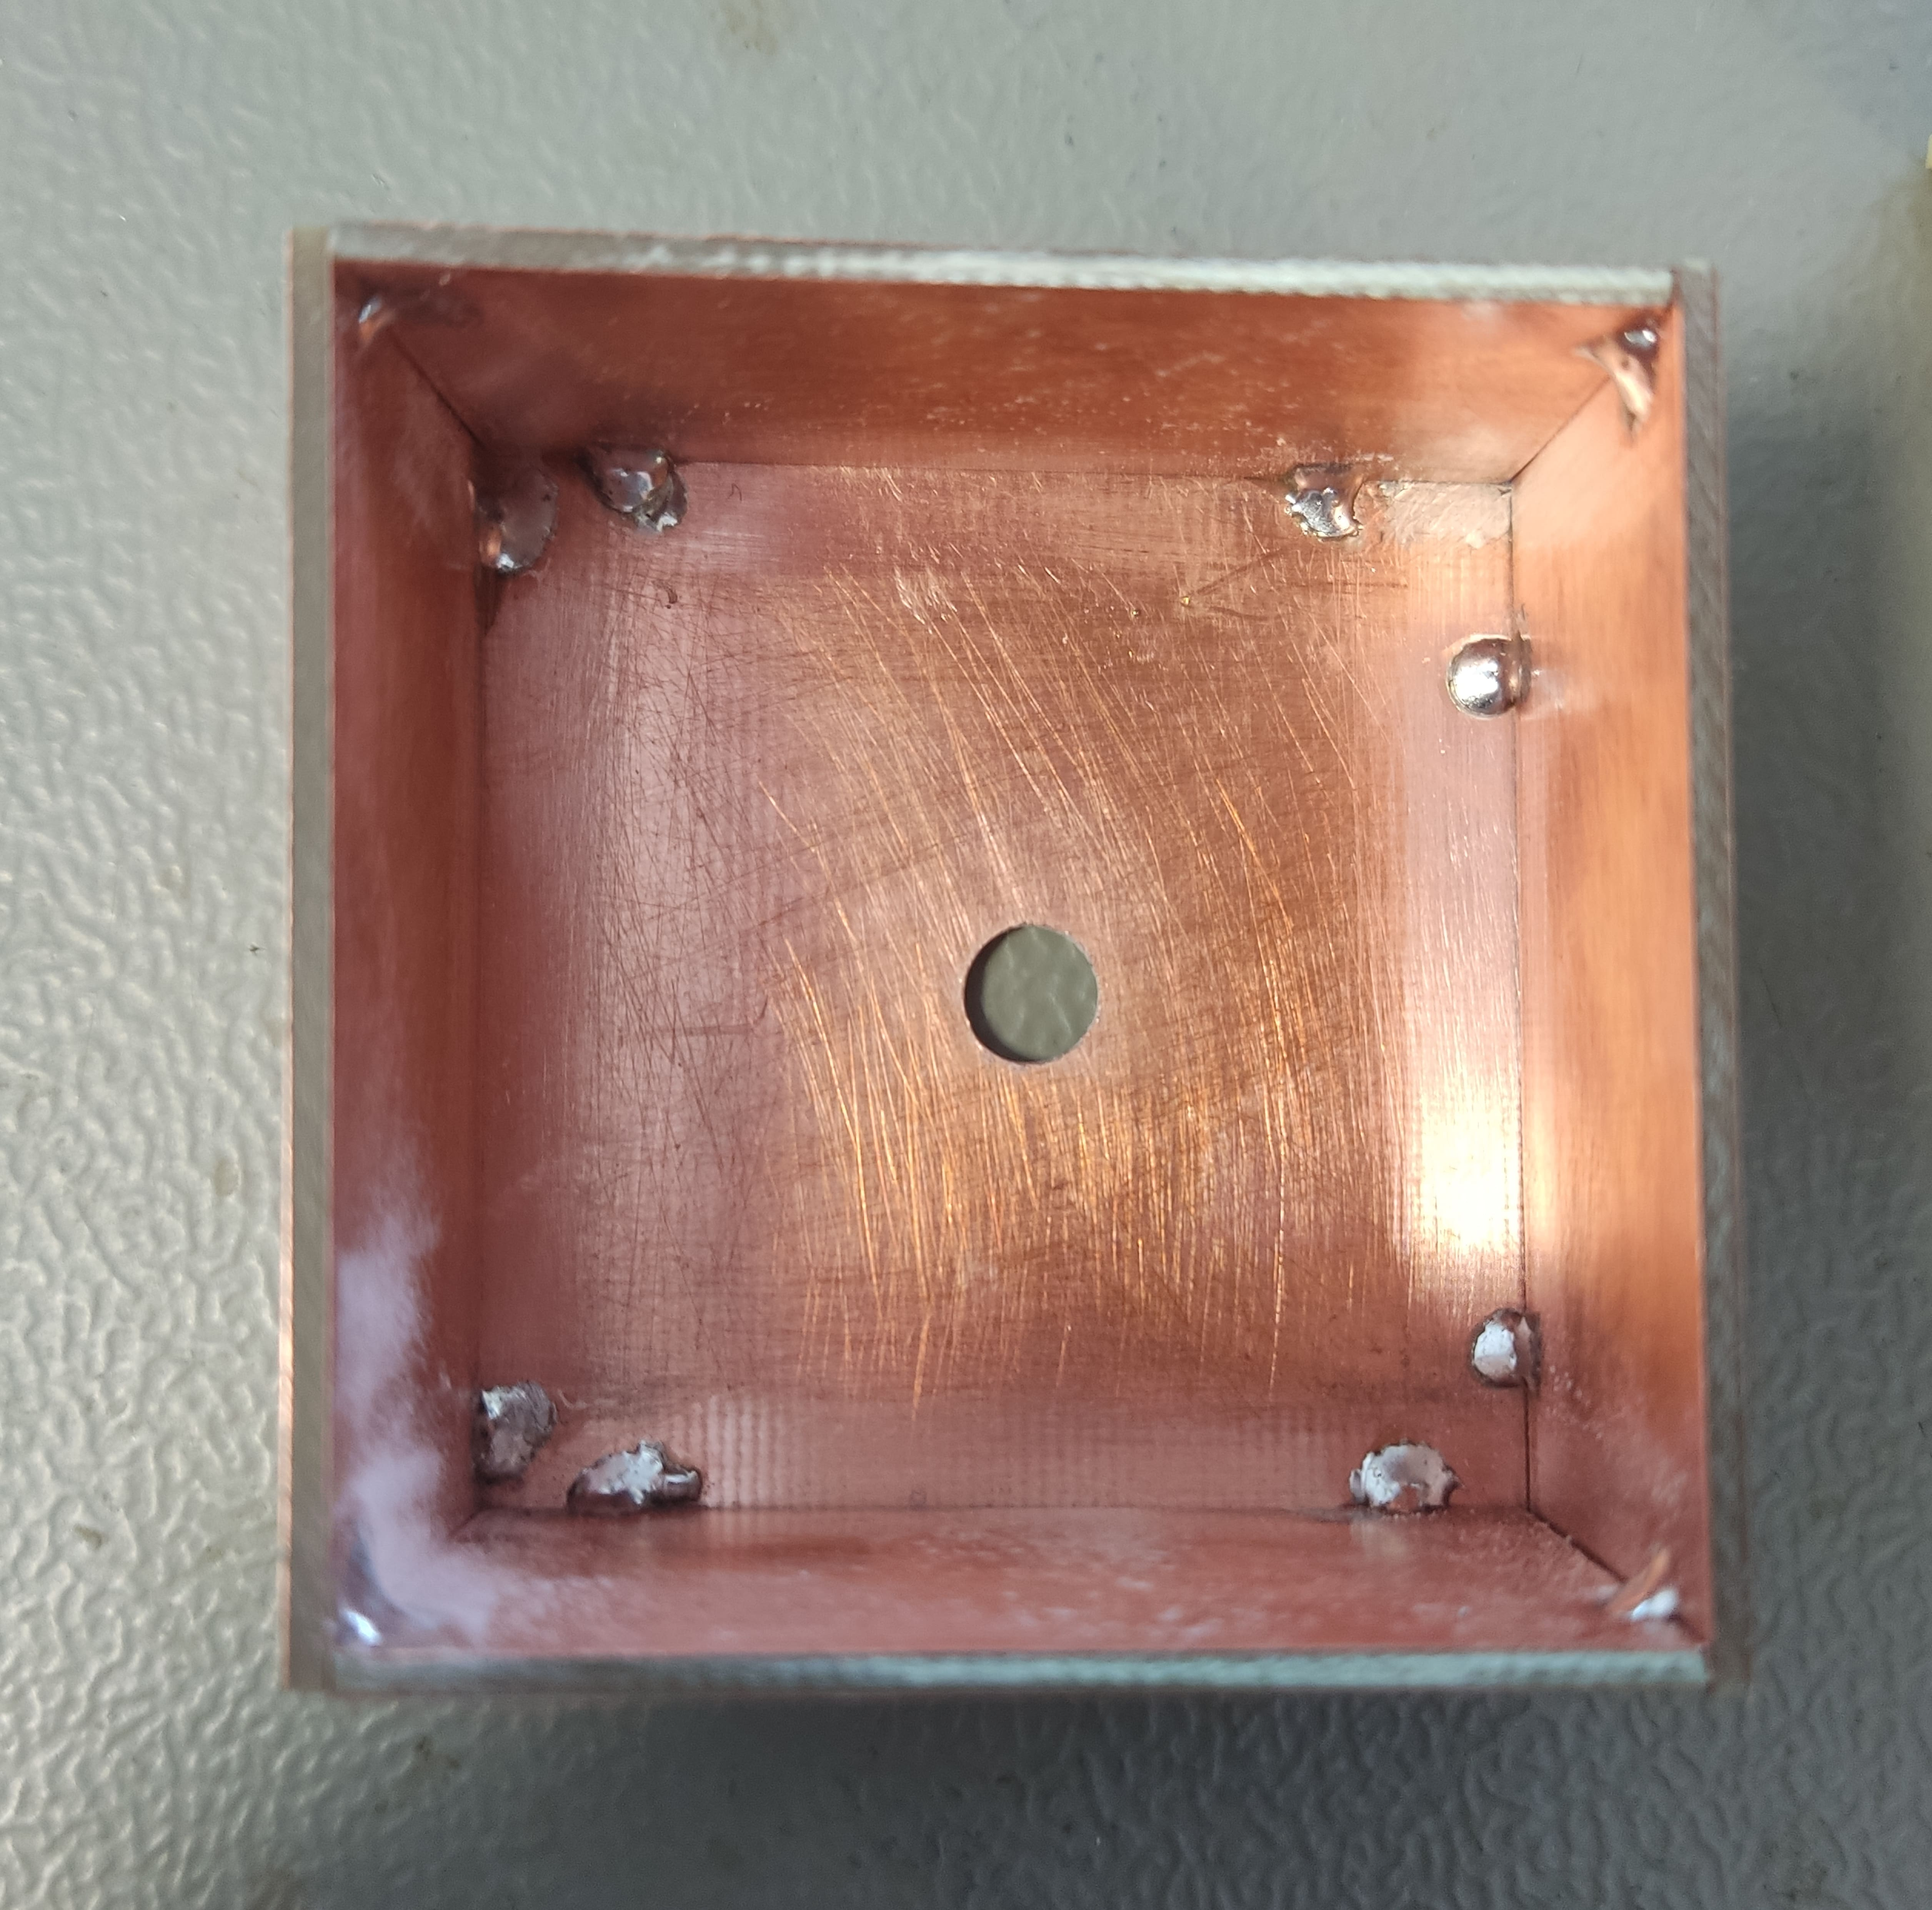
\includegraphics[width=0.3\linewidth]{figs/ch3_antenna1Box.jpg}
    \caption{Box part of antenna 1}
    \label{fig:ch3_antenna1Box.jpg}
\end{figure}

\par The antenna was fed by coaxial cable that would terminate in a front panel connector, as mentioned above. This can be seen in Figure \ref{fig:ch3_antennaFeedBack.png} and Figure \ref{fig:ch3_antennaFeedFront.png}.

\begin{figure}[H]
    \vspace*{0cm}
    \centering
    \includegraphics[width=0.3\linewidth]{figs/ch3_antennaFeedBack.png}
    \caption{Back side of antenna \ac{pcb} with feed cable}
    \label{fig:ch3_antennaFeedBack.png}
\end{figure}

\begin{figure}[H]
    \vspace*{0cm}
    \centering
    \includegraphics[width=0.3\linewidth]{figs/ch3_antennaFeedFront.png}
    \caption{Front side of antenna \ac{pcb} with feed point}
    \label{fig:ch3_antennaFeedFront.png}
\end{figure}

\par Both sides of antenna 1 were then glued together using commonly available super glue. Subsequently, the antenna was tested with a Keysight N9918A FieldFox Handheld Microwave Analyzer in the laboratories of Instituto de Telecomunicações, as seen in Figure \ref{fig:ch3_antenna1Testing.png}. The measured S11 results of this antenna can be seen in Figure \ref{fig:ch3_s11magAnt1.png}. We first started by calibrating the equipment and then captured the relevant values in the frequency range of $[1.5, 3.0] \:\si{GHz}$.

\begin{figure}[H]
    \vspace*{0cm}
    \centering
    \includegraphics[width=0.4\linewidth]{figs/ch3_antenna1Testing.png}
    \caption{S11 Magnitude results for antenna 1}
    \label{fig:ch3_antenna1Testing.png}
\end{figure}

\begin{figure}[H]
    \vspace*{0cm}
    \centering
    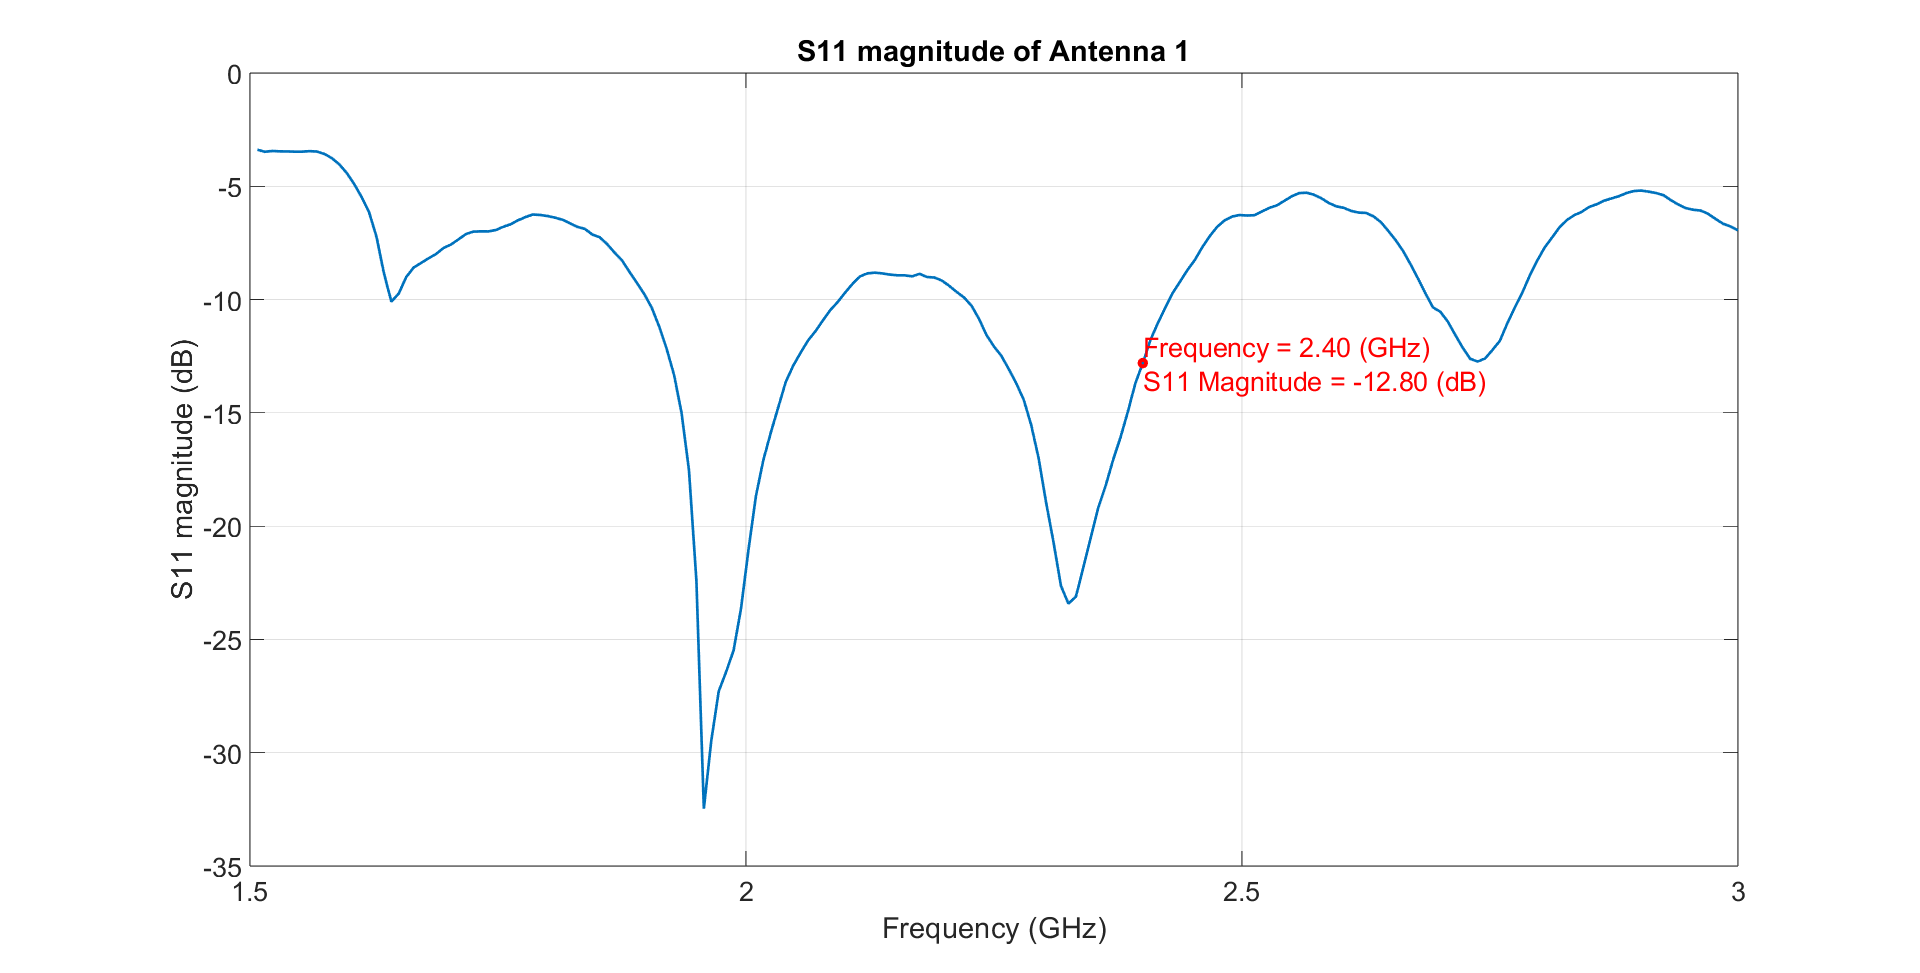
\includegraphics[width=1\linewidth]{figs/ch3_s11magAnt1.png}
    \caption{Testing of antenna 1}
    \label{fig:ch3_s11magAnt1.png}
\end{figure}

\par As can be seen, the results for this antenna were not what was expected from the simulations done on CST Studio. The S11 parameter is barely below the $-10 \:\si{dB}$ threshold, a value of $-12.80\:\si{dB}$ at a frequency of $2.4\:\si{GHz}$, and the overall response of antenna 1 was not good. After careful consideration, it was argued that maybe adding more soldering points inside the box could be beneficial, as it was suspected that the radiation from the backside of the antenna could be causing abnormal currents on the box's copper surface, and thus destroying the antenna's response. After this theory was proposed, the antenna 2 box was assembled and more solder points were added to the back portion of the box to achieve better results. The interior of the antenna 2 box can be seen in Figure \ref{fig:ch3_antenna2Box.jpg}.

\begin{figure}[H]
    \vspace*{0cm}
    \centering
    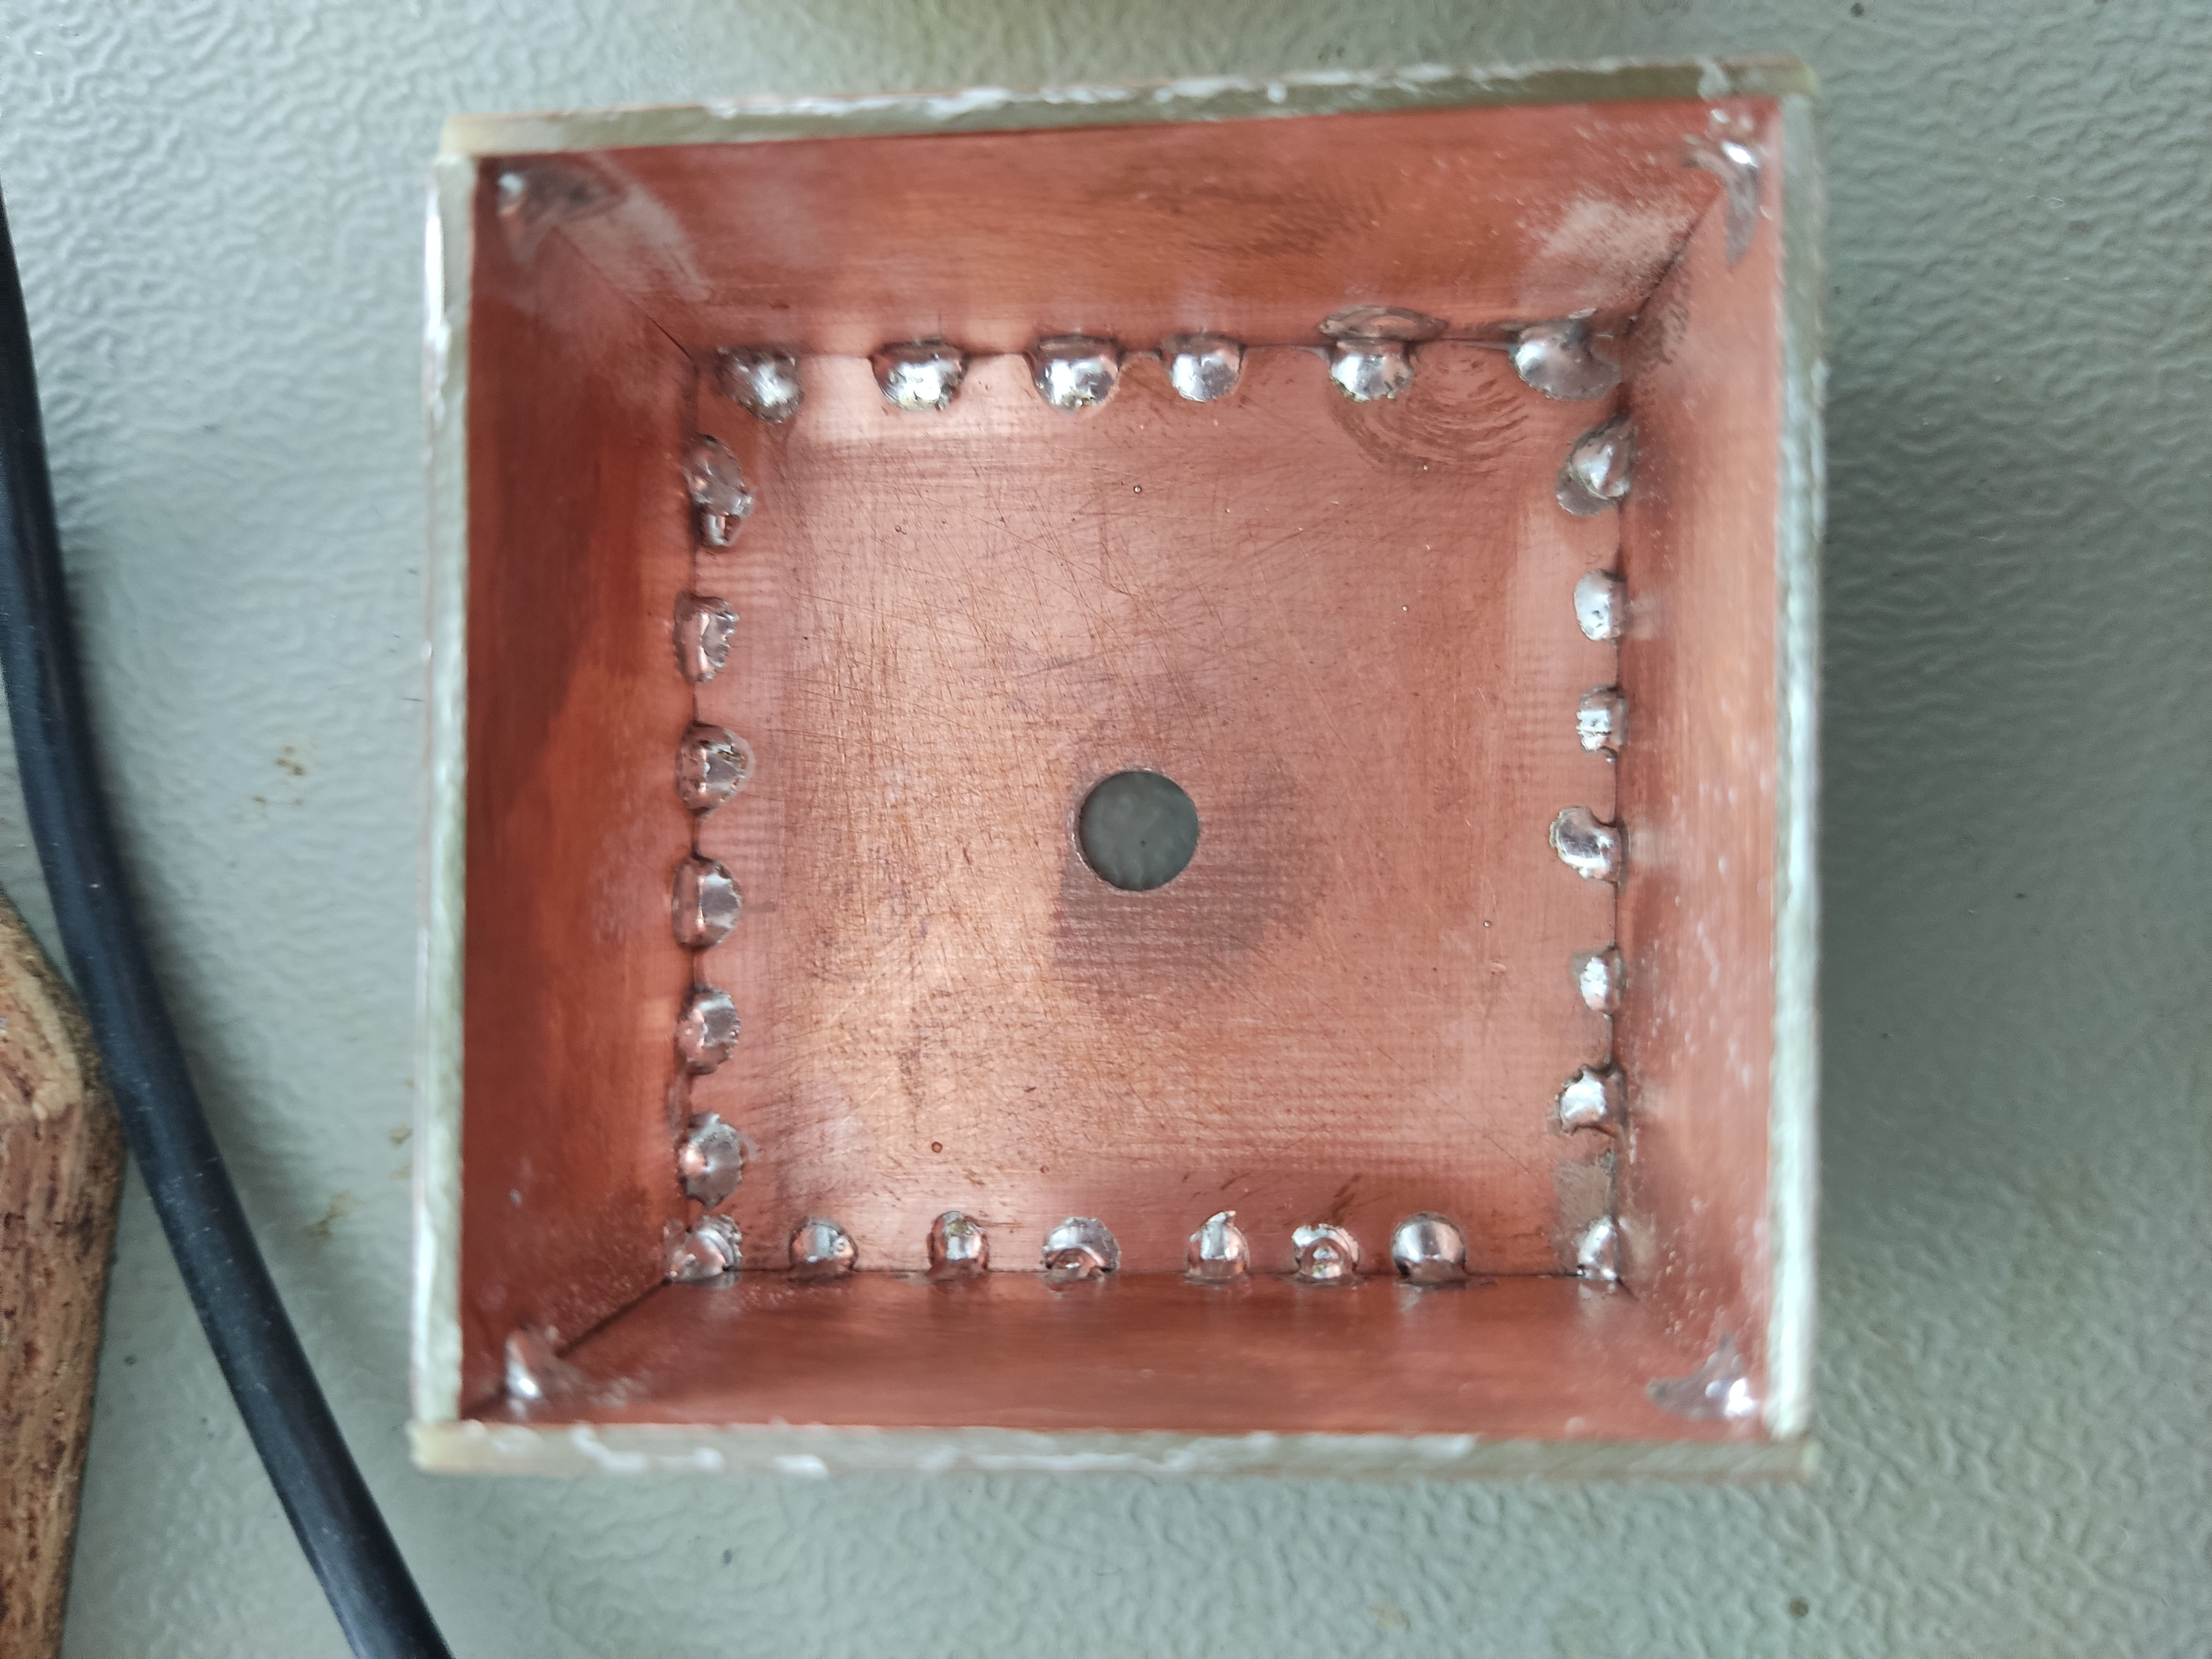
\includegraphics[width=0.3\linewidth]{figs/ch3_antenna2Box.jpg}
    \caption{View from the inside of antenna 2 box}
    \label{fig:ch3_antenna2Box.jpg}
\end{figure}

\par Antenna 2 has, in fact, better S11 Magnitude values, seen in Figure \ref{fig:ch3_s11magAnt2.png}, than antenna 1. This can be due to a variety of factors, as these antennas and the box behind them were hand made so there will differences in their construction. It cannot be determined that simply adding the extra solder points are the reason behind the improvements seen in antenna 2.

\begin{figure}[H]
    \vspace*{0cm}
    \centering
    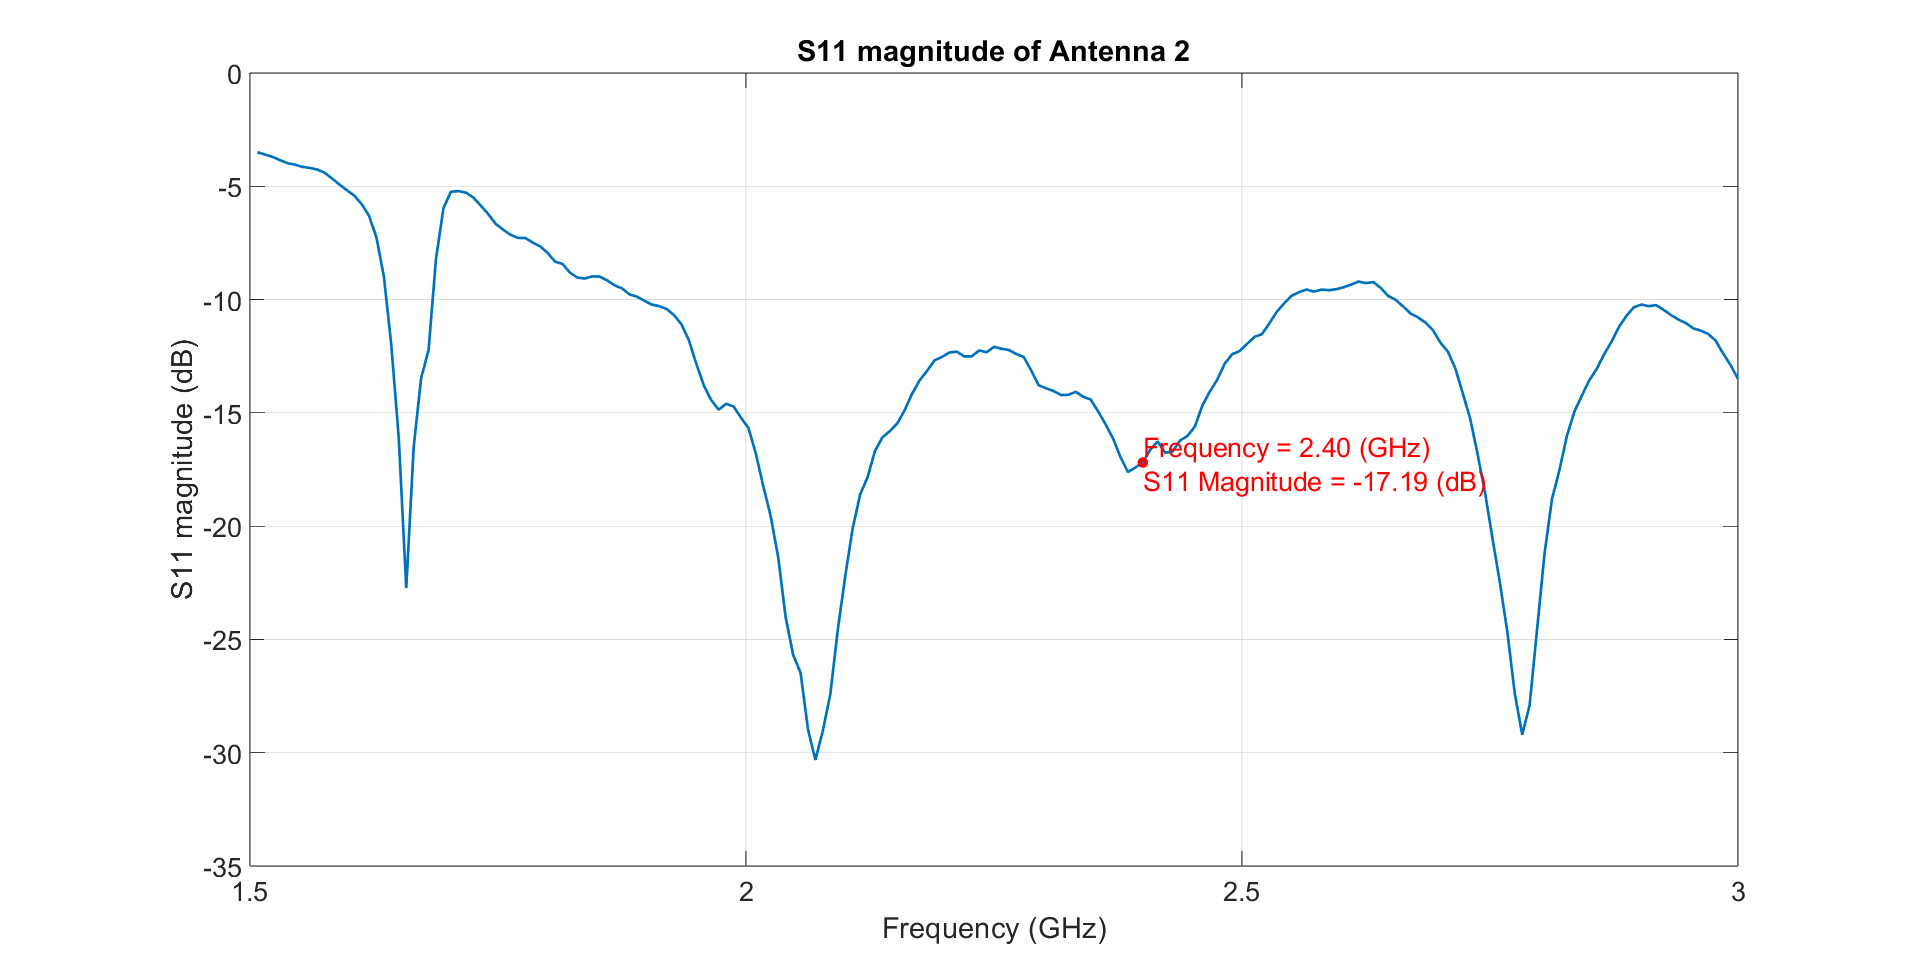
\includegraphics[width=1\linewidth]{figs/ch3_s11magAnt2.png}
    \caption{S11 Magnitude results for antenna 2}
    \label{fig:ch3_s11magAnt2.png}
\end{figure}

\par The response of antenna 2 has a larger portion of its S11 Magnitude below the $-10\:\si{dB}$ mark, managing to achieve a value of $-17.19\:\si{dB}$ at the $2.4\:\si{GHz}$ frequency. These results are also much closer to the simulated Magnitude of the S11 parameter done in CST Studio. This results in a more suitable antenna for application on the project.
\chapter{Result Analysis of the Circuit}
\label{chapter:testing}

\par In this chapter the methodology used for testing the prototype is presented. 

\section{Test Setup}
\par The testing for this project was carried out in a laboratory of the Instituto de Telecomunicações. The equipment used is listed below.

\begin{itemize}
    \item PL303QMT-P power supply;
    \item SMR40 Signal Generator;
    \item FSH13 Spectrum Analyzer;
    \item AFG31000 Series Arbitrary Function Generator;
    \item Fluke Multimeter
\end{itemize}

\par In order not to potentially damage any equipment during testing, two \ac{rf} attenuators were used. The first was the BW-N10W50 + from Mini-Circuits that has an attenuation of $10\:\si{dB}$ and is rated at $50\:\si{W}$ and the second was the VAT-20W2 + also from Mini-Circuits with an attenuation of $20\:\si{dB}$ rated at a power of $2\:\si{W}$.

\par With these, even if the circuit reaches its full expected power output of $40\:\si{dBm}$, we would still be within the safe range of operation of the FSH13 spectrum analyzer, which can have inputs of up to $20\:\si{dBm}$. This analyzer was configured to also have an attenuation of $10\:\si{dB}$ throughout the tests that were carried out.

\par The power supply that was used has three outputs named Output 1, 2 and 3. In order to obtain the necessary voltage values for the circuit, Output 3 would be used for the voltage $V_{G}$ and Output 2 for $V_{D}$. Output 1 would not be used.

\par The positive terminal of Output 3 was short-circuited to the negative terminal of Output 2. This allowed us the use a single ground wire from the power supply, and having Output 3 produce the negative voltage levels needed for $V_{G}$ and Output 2 would be responsible for the positive voltages used for both $V_{D}$ and the $28V$ supply voltage.

\par The Spectrum Analyzer was configured to be centered on $2.4\:\si{GHz}$ and a span of $40\:\si{MHz}$. This would allow us to see the carrier frequency and the \ac{i} and \ac{q} components of the signal.

\section{Bias Sequency of the circuit}
\par The circuit has to respect the turning ON and OFF protocol established by the manufacturer of \ac{pa} used.

\par To turn on the circuit we first need to ensure that $V_{G}$ is set to $-5 \:\si{V}$. We can then turn on Output 2 of the power supply at $28\:\si{V}$. Subsequently, we increase $V_{G}$ until $I_{DS}$ has the intended value. After this procedure we can finally supply the desired \ac{rf} signal.

\par To power the circuit, we start by turning off the \ac{rf} signal. We then decrease $V_{G}$ until the pinch-off value of $-5\:\si{V}$ is reached. The value of $V_{D}$ is then decreased to $0\:\si{V}$. After these steps we can finally turn off $V_{G}$.

\section{Buck Converter}
\par We first tested the buck converter. To do so, the \ac{pa} was kept turned off. After initial debugging, which included resoldering the two resistors responsible for setting the output voltage value, and adding a missing short-circuit resistor, the power supply output was measured with the multimeter at a voltage of $3.25\:\si{V}$ at its output. The buck converter had an absolute error of $0.05\:\si{V}$ and a relative error of just  $1.5\%$. Although not the expected $3.3\:\si{V}$, this value is close enough that we were not concerned with continuing the tests.

\par The current consumed at this stage was of $36\:\si{mA}$ for a supply voltage of $28\:\si{V}$. The setup used for this point is shown in Figure \ref{fig:ch4_psuTesting.jpg}. Note that all \ac{rf} ports are terminated on $50\:\si{\Omega}$ impedances.

\begin{figure}[H]
    \vspace*{0cm}
    \centering
    \includegraphics[width=0.7\linewidth]{figs/ch4_psuTesting.jpg}
    \caption{Testing of the Buck Converter Setup}
    \label{fig:ch4_psuTesting.jpg}
\end{figure}


\section{Testing of the Prototype}
\par Following the appropriate biasing protocol mentioned above, we started to record the values of current and $V_{G}$. Figure \ref{fig:ch4_npa1007Pol.png} shows the logged data for this part.

\begin{figure}[H]
    \vspace*{0cm}
    \centering
    \includegraphics[width=1\linewidth]{figs/ch4_npa1007Pol.png}
    \caption{Testing of the Project Setup}
    \label{fig:ch4_npa1007Pol.png}
\end{figure}

\par We have to note that above a current of $140 \:\si{mA}$ it was noticed that the \ac{pa} would enter thermal runaway. As such, without proper heat dissipation techniques, it is dangerous to allow the circuit to work at certain polarizations without having the current limited in the power supply.

\par In order to test the circuit response to a power input, we tried a setup similar to the one of Figure \ref{fig:ch4_fullSetup.jpg}. The only difference being that the connectors for the \ac{i} and \ac{q} would be terminated by $50\:\si{\Omega}$ loads.

\begin{figure}[H]
    \vspace*{0cm}
    \centering
    \includegraphics[width=1\linewidth]{figs/ch4_fullSetup.jpg}
    \caption{Testing of the Prototype Setup}
    \label{fig:ch4_fullSetup.jpg}
\end{figure}

\par We proceeded to record the output power delivered by the circuit when supplied with a given input power. The data is presented on Figure \ref{fig:ch4_AMAM.png} in the form of an AM/AM plot.

\begin{figure}[H]
    \vspace*{0cm}
    \centering
    \includegraphics[width=1\linewidth]{figs/ch4_AMAM.png}
    \caption{Testing of the Project Setup using an atenuation of $40 \:\si{dB}$}
    \label{fig:ch4_AMAM.png}
\end{figure}

\par This graph reveals a severe lack of gain on the output signal. Even with a series of attenuators, and the attenuation of the Spectrum Analyzer, the graph shows that the output is delivering an insignificant amount of power. For a maximum input power of $16\:\si{dBm}$, we can see that the output power measured on the Spectrum Analyzer was around $-47\:\si{dBm}$. This output power had been atenuated by $40 \:\si{dB}$, meaning that the actual power at the output of the prototype would be $-7\:\si{dBm}$. There is a possibility that the power being measured at the output of the circuit is nothing more than the leakage power.

\par Next, we tried to repeat the process, only this time with the signals \ac{i} and \ac{q}. We used signals of $2.8\:\si{V}$ of amplitude, centered on $1.4\:\si{V}$ with various frequency values, ranging from $1\:\si{MHz}$ to $2\:\si{0MHz}$. The test setup for the part is as shown in Figure \ref{fig:ch4_fullSetup.jpg}.

\par Unfortunately, there was no change in the circuit response, and we could not verify the presence of any modulation on the output through the Spectrum Analyzer.

\par After suspecting that the problem lay on the quadrature modulator, it was decided to measure the values of the input signals of the modulator, with the inputs terminated on $50\:\si{\Omega}$ loads. Pins 8, 9, 10 and 11 of the modulator read voltages of $[3.292 0.085 2.249 0.247]\:\si{V}$. These values are not consistent with what was expected to be present, showing that the modulator is not working as expected. 

\par We tried to resolder the component in hopes that it would work, but these efforts were in vain. It was then impossible to fully test the circuit. Unfortunately, after the problem was identified and a last resolver attempt was made, there was no more time left to search for another component and make the necessary changes to use another \ac{iq} modulator. As such, solving this issue has to be done in a future prototype.
\chapter{Conclusion}
\label{chapter:conclusion}

\par Throughout the duration of this project, the main goal was to design and implement a prototype for an element of a modular \ac{psa}. The idea was that this element could be replicated and organized in a side-by-side configuration. 

\par The element should contain all the necessary components for its operation while having a limited number of connections to the outside.

\par The prototype had a set of two \ac{pcb}s of small dimensions that could be placed inside a case that had the same height and width as the antenna that was designed. This requirement imposed restrictions on the design of the \ac{pcb}s and on the interconnections between boards and connectors, which were successfully met.

\par The antenna that was designed proved to be difficult to replicate, as although the last one to be assembled had characteristics that respected the specifications, the first antenna produced was slightly below the desired specification. This experience highlighted the potential of the design, and now the significant effort and skill required to consistently replicate the antennas with similar characteristics is understood.

\par A \ac{smps} was used in order to convert the $28\:\si{V}$ that were supplied to the element into the $3.3\:\si{V}$ that most of its internal components, with the exception of the \ac{pa}, used. It was crucial to deliver power to the element at the desired voltage.

\par Although some issues related to the \ac{iq} Modulator arised, limiting the ability to verify the prototype's complete operation, a small amount of power could be measured at a frequency of $2.4\:\si{GHz}$ while testing. This signal, due to its low power, could have been leakage power from the \ac{iq} Modulator. This, combined with the fact that the \ac{i} and \ac{q} components of the modulator did not seem to produce any effect on the \ac{pa} output signal, meant that the prototype could not achieve the desired output power of $[5, 10] \:\si{W}$ nor modulate signals.

\par After aquiring all components and assembling the \ac{pcb}s, the testing phase revealed additional areas for improvement, such as an oversight regarding the $-10\:\si{dB}$ of the \ac{iq} Modulator and the low output P1dB $17.6 \:\si{dBm}$ of the driver amplifier. These findings provide useful information for adjustments in the next prototype.

\par This prototype, although not having met all initial requirements, was useful to better understand that a more careful approach to the choice of components for a new iteration of this prototype must be taken, particularly with regard to the adequacy of the \ac{ic} soldering requirements to the techniques available in the laboratory facilities. This work provides a valuable insight that can lead future iterations of the project to success.

%%%%%%%%%%%%%%%%%%%%%%%%%%%%%%%%%%%%%%%%%%%%%%%%%%%%%%%
% End of Thesis text 
%%%%%%%%%%%%%%%%%%%%%%%%%%%%%%%%%%%%%%%%%%%%%%%%%%%%%%%

\backmatter

%%%%%%%%%%%%%%%%%%%%%%%%%%%%%%%%%%%%%%%%%%%%%%%%%%%%%%%
% Print all used references
%%%%%%%%%%%%%%%%%%%%%%%%%%%%%%%%%%%%%%%%%%%%%%%%%%%%%%%

\begingroup
\renewcommand{\bibfont}{\footnotesize}
% Redefine References name to Portuguese
% Change if you are using english
\defbibheading{bibliography}[References]{
	\chapter{#1}
}
\SingleSpacing
\setlength\bibitemsep{8pt}
\printbibliography[heading=bibliography]
\endgroup


%%%%%%%%%%%%%%%%%%%%%%%%%%%%%%%%%%%%%%%%%%%%%%%%%%%%%%%
% Load appendix
%%%%%%%%%%%%%%%%%%%%%%%%%%%%%%%%%%%%%%%%%%%%%%%%%%%%%%%

\mainmatterWithoutReset
\appendix

% \include{appendix-a}
% \include{appendix-b}
% \include{appendix-c}

\end{document}
